\documentclass[12pt]{article}
\usepackage{amsmath, amssymb, amsthm}
\usepackage{tikz}
\usetikzlibrary{arrows.meta}
\usepackage[margin=1in]{geometry}
\usepackage{asymptote}
\usepackage{graphicx}

\newtheorem{theorem}{Theorem}
\newtheorem{lemma}[theorem]{Lemma}
\newtheorem{proposition}[theorem]{Proposition}
\newtheorem{corollary}[theorem]{Corollary}
\newtheorem{definition}[theorem]{Definition}
\theoremstyle{remark}
\newtheorem{remark}[theorem]{Remark}

\title{A Structural Characterisation of the $3\times3$ Magic Square of Squares}
\author{Shaimaa Said Soltan}
\date{\today}

\begin{document}
\maketitle

\begin{abstract}
We give a complete parametrisation of the family of $3\times3$ magic
squares, expressed so as to isolate the arithmetic difficulty in the
problem of nine distinct perfect squares. Writing the nine cells in
terms of three free parameters, we show that the linear system defining
the family has rank $6$ and nullity $3$, and we exhibit an explicit
basis for its solution space. We identify a distinguished triple of
\emph{anchors} $(E^2, I^2, X)$ in terms of which three of the cells take
a symmetric form, and show that the resulting configuration is the
medial triangle of the cells it determines. Normalising by scale and
translation reduces the configuration to a one-parameter family. We
then locate the obstruction to a nine-square solution precisely: it is
the requirement that $2E^2$ admit four essentially distinct
representations as a sum of two squares, subject to one additional
linear condition. Finally we prove that no linear relation among the
cells can obstruct a nine-square solution, which explains why purely
algebraic approaches to the problem do not close.
\end{abstract}

\section{Setup}

Label the $3\times3$ square
\[
\begin{array}{|c|c|c|}
\hline
A^2 & B^2 & C^2 \\ \hline
D^2 & E^2 & F^2 \\ \hline
X   & H^2 & I^2 \\ \hline
\end{array}
\]
where $E^2$ denotes the centre and $X$ the bottom-left cell. The
notation records our intended application --- that the entries be
perfect squares --- but no such assumption is made in
Sections~\ref{sec:param}--\ref{sec:norm}, where all results hold for
arbitrary real entries satisfying the magic condition.

\section{The Parametrisation}\label{sec:param}

\begin{proposition}\label{prop:param}
Every $3\times3$ magic square is determined by $A^2$, $E^2$ and $X$
through
\begin{align}
C^2 &= 2E^2 - X, \label{eq:C}\\
I^2 &= 2E^2 - A^2, \label{eq:I}\\
B^2 &= E^2 - A^2 + X, \label{eq:B}\\
H^2 &= E^2 + A^2 - X, \label{eq:H}\\
D^2 &= 3E^2 - A^2 - X, \label{eq:D}\\
F^2 &= A^2 + X - E^2, \label{eq:F}
\end{align}
and its magic sum is $3E^2$.
\end{proposition}

\begin{proof}
The eight line conditions are linear in the nine cells. Solving the
diagonal, the first column and the first row successively for $I^2$,
$X$-complement and $C^2$ yields \eqref{eq:C}--\eqref{eq:F}; each
remaining line is then satisfied identically.
\end{proof}

\begin{corollary}[Opposite pairs]\label{cor:pairs}
Each pair of cells symmetric about the centre averages to it:
\[
A^2 + I^2 = B^2 + H^2 = C^2 + X = D^2 + F^2 = 2E^2 .
\]
\end{corollary}

Consequently every line consists of the centre together with one
opposite pair, and sums to $E^2 + 2E^2 = 3E^2$.

\section{Relations Satisfied by $B^2$}

Since $B^2$ is determined by the parameters, it may be written in terms
of each of the remaining cells:
\begin{align}
B^2 &= E^2 - A^2 + X, & B^2 &= 3E^2 - A^2 - C^2, \notag\\
B^2 &= E^2 - C^2 + I^2, & B^2 &= 2I^2 - D^2, \notag\\
B^2 &= 2E^2 - 2A^2 + F^2, & B^2 &= -A^2 + F^2 + I^2, \notag\\
B^2 &= 2X - F^2, & B^2 &= 2E^2 - H^2. \notag
\end{align}
As a coefficient matrix over the ordered basis
$(E^2, A^2, C^2, D^2, F^2, X, H^2, I^2)$ these read
\[
M =
\begin{pmatrix}
1 & -1 &  0 &  0 &  0 & 1 &  0 & 0 \\
3 & -1 & -1 &  0 &  0 & 0 &  0 & 0 \\
1 &  0 & -1 &  0 &  0 & 0 &  0 & 1 \\
0 &  0 &  0 & -1 &  0 & 0 &  0 & 2 \\
2 & -2 &  0 &  0 &  1 & 0 &  0 & 0 \\
0 & -1 &  0 &  0 &  1 & 0 &  0 & 1 \\
0 &  0 &  0 &  0 & -1 & 2 &  0 & 0 \\
2 &  0 &  0 &  0 &  0 & 0 & -1 & 0
\end{pmatrix}.
\]

\begin{lemma}
Every row of $M$ has coefficient sum $1$.
\end{lemma}

\begin{proof}
The constant square, with all nine entries equal to $t$, is magic.
Substituting it into any valid relation gives
$t = \bigl(\sum_j m_{ij}\bigr) t$ for all $t$.
\end{proof}

The row sums therefore serve as a consistency check on any derived
relation. Moreover $\det M = 0$: for instance
$r_5 + r_7 = 2r_1$, since
$(2E^2 - 2A^2 + F^2) + (2X - F^2) = 2(E^2 - A^2 + X)$.

\begin{proposition}\label{prop:rank}
The system \eqref{eq:C}--\eqref{eq:F} has rank $6$ and nullity $3$.
Every linear relation holding on the family is a linear combination of
these six, and a basis for the solution space, in coordinates
$(E^2, A^2, C^2, D^2, F^2, X, H^2, I^2; B^2)$, is
\begin{align*}
v_1 &= (1,0,2,3,-1,0,1,2;\,1),\\
v_2 &= (0,1,0,-1,1,0,1,-1;\,-1),\\
v_3 &= (0,0,-1,-1,1,1,-1,0;\,1).
\end{align*}
\end{proposition}

\begin{remark}
Any further relation derived from the system --- however many
substitutions it involves, and whatever constant multiple of $E^2$ it
closes at --- is by Proposition~\ref{prop:rank} a combination of the
six. It is therefore an identity on the family, valid for every magic
square, and imposes no condition.
\end{remark}

\section{The Anchors $(E^2, I^2, X)$}\label{sec:anchors}

By Corollary~\ref{cor:pairs}, each of $E^2$, $I^2$, $X$ is the mean of a
pair drawn from $\{B^2, D^2, F^2\}$:
\[
D^2 + F^2 = 2E^2, \qquad B^2 + D^2 = 2I^2, \qquad B^2 + F^2 = 2X .
\]
Solving for the cells gives the symmetric form
\begin{align}
B^2 &= -E^2 + I^2 + X, \label{eq:Ba}\\
D^2 &= \phantom{-}E^2 + I^2 - X, \label{eq:Da}\\
F^2 &= \phantom{-}E^2 - I^2 + X, \label{eq:Fa}
\end{align}
the three expressions differing only in the placement of the minus
sign. The remaining cells follow as $A^2 = 2E^2 - I^2$,
$C^2 = 2E^2 - X$ and $H^2 = 2E^2 - B^2$, so $(E^2, I^2, X)$ may be
taken as free parameters in place of $(A^2, E^2, X)$.

\begin{proposition}[Medial configuration]
If $B^2$, $D^2$, $F^2$ are taken as the vertices of a triangle, then
$I^2$, $X$, $E^2$ are the midpoints of the edges $B^2D^2$, $B^2F^2$ and
$D^2F^2$ respectively. Each cell is the sum of the two anchors incident
to it, minus the anchor on the opposite edge.
\end{proposition}

Differencing the identities eliminates the shared cell and doubles the
remaining anchors:
\[
B^2 - D^2 = 2(X - E^2), \quad
B^2 - F^2 = 2(I^2 - E^2), \quad
D^2 - F^2 = 2(I^2 - X).
\]
Thus differences of cells are twice the corresponding differences of
anchors, and each anchor comparison mirrors a cell comparison: for
example $I^2 > X$ precisely when $D^2 > F^2$. The relation
$B^2 - F^2 = 2(I^2 - E^2)$ is the midline theorem for the triangle
above.

\section{Normalisation}\label{sec:norm}

The configuration has three degrees of freedom; removing scale and
translation leaves one. Place $F^2$ at the origin and $B^2$ at $1$, and
set
\[
t = \frac{D^2 - F^2}{B^2 - F^2}.
\]

\begin{center}
\begin{tabular}{lcl}
\hline
Point & Position & Origin \\
\hline
$F^2$ & $0$       & endpoint \\
$E^2$ & $t/2$     & midpoint of $D^2, F^2$ \\
$X$   & $1/2$     & midpoint of $F^2, B^2$ \\
$D^2$ & $t$       & free parameter \\
$I^2$ & $(1+t)/2$ & midpoint of $D^2, B^2$ \\
$B^2$ & $1$       & endpoint \\
\hline
\end{tabular}
\end{center}

Two features are independent of $t$: the anchor $X$ is fixed at $1/2$,
and $I^2 - E^2 = 1/2$, so $E^2$ and $I^2$ remain a fixed half-unit
apart as $t$ varies. The remaining gaps are $I^2 - X = t/2$ and
$X - E^2 = (1-t)/2$. The values $t = 0$ and $t = 1$ are excluded, as
they force $D^2 = F^2$ and $D^2 = B^2$ respectively.

\begin{center}
\begin{tikzpicture}[x=1cm,y=1cm]
  \draw[gray] (-4,0) -- (12.4,0);
  \foreach \p/\n in {0/F^2, 8.407/D^2, 12/B^2}
    {\fill (\p,0) circle (2.6pt); \node[above] at (\p,0.35) {$\n$};}
  \foreach \p/\n in {4.204/E^2, 6/X, 10.204/I^2}
    {\fill[gray] (\p,0) circle (2.6pt); \node[below] at (\p,-0.1) {$\n$};}
  \foreach \p/\n in {0/0, 8.407/{t}, 12/1}
    {\node[blue] at (\p,0.3) {\footnotesize $\n$};}
  \fill[red] (-1.796,0) circle (2.6pt);
  \node[above,red] at (-1.796,0.35) {$A^2$};
  \fill[purple] (2.407,0) circle (2.6pt);
  \node[above,purple] at (2.407,0.35) {$C^2$};
  \fill[brown] (-3.593,0) circle (2.6pt);
  \node[above,brown] at (-3.593,0.35) {$H^2$};
  \draw[red] (-3.593,-0.4) -- (-1.796,-0.4);
  \node[below,red] at (-2.7,-0.5) {\footnotesize $\delta_{\text{norm}}$};
  \draw[red] (-1.796,-0.4) -- (0,-0.4);
  \node[below,red] at (-0.9,-0.5) {\footnotesize $\delta_{\text{norm}}$};
  \draw[red] (2.407,-0.4) -- (4.204,-0.4);
  \node[below,red] at (3.3,-0.5) {\footnotesize $\delta_{\text{norm}}$};
  \draw[red] (8.407,-0.4) -- (10.204,-0.4);
  \node[below,red] at (9.3,-0.5) {\footnotesize $\delta_{\text{norm}}$};
  \draw[red] (10.204,-0.4) -- (12,-0.4);
  \node[below,red] at (11.1,-0.5) {\footnotesize $\delta_{\text{norm}}$};
  \draw (0,-1.1) -- (12,-1.1);
  \fill[gray] (6,-1.1) circle (2.6pt);
  \node[below] at (6,-1.2)
    {\footnotesize $X$ midway between $F^2$ and $B^2$};
  \draw (8.407,-2.2) -- (12,-2.2);
  \fill[gray] (10.204,-2.2) circle (2.6pt);
  \node[below] at (9.8,-2.3)
    {\footnotesize $I^2$ midway between $D^2$ and $B^2$};
  \draw (0,-3.3) -- (8.407,-3.3);
  \fill[gray] (4.204,-3.3) circle (2.6pt);
  \node[below] at (4.204,-3.4)
    {\footnotesize $E^2$ midway between $D^2$ and $F^2$};
  \draw[red] (4.204,-4.4) -- (6,-4.4);
  \node[below,red] at (5.1,-4.5)
    {\footnotesize $\delta_{\text{norm}} = (1-t)/2$};
  \draw[orange] (6,-5.5) -- (8.407,-5.5);
  \node[below,orange] at (7.2,-5.6)
    {\footnotesize $\sigma_{\text{norm}} = t - 1/2$};
  \draw[orange] (0,-6.6) -- (2.407,-6.6);
  \node[below,orange] at (1.2,-6.7)
    {\footnotesize $\sigma_{\text{norm}}$};
\end{tikzpicture}
\end{center}

Here $\delta_{\text{norm}}$ and $\sigma_{\text{norm}}$ are the
normalised (dimensionless) gap sizes on the $[0,1]$ line; the
corresponding real quantities, in cell units, are
$\delta_{\text{real}} = X - E^2 = \delta_{\text{norm}}\cdot S$ and
$\sigma_{\text{real}} = D^2 - X = \sigma_{\text{norm}}\cdot S$, with
$S = B^2 - F^2$ as in the de-normalised form above. The last gap,
$\sigma_{\text{norm}} = t - 1/2$, is the one segment of the six not
already accounted for by a midpoint or by $\delta_{\text{norm}}$; for
the square of Section~\ref{sec:ex}, $\sigma_{\text{real}} = 55608$.
The same length reappears elsewhere on the line:
$\sigma_{\text{real}} = C^2 - F^2$ as well, since $C^2$'s normalised
position is $t - 1/2 = \sigma_{\text{norm}}$ directly
(Section~\ref{sec:norm}'s de-normalised form places $F^2$ at the
origin).

\paragraph{Two more reflections: $C^2$ and $H^2$.}
The mechanism that placed $A^2 = 2E^2 - I^2$ on the line works for the
other two opposite-pair partners not yet plotted. Since
$C^2 = 2E^2 - X$,
\[
C^2 = F^2 + \left(t - \tfrac12\right)S,
\]
which places $C^2$ \emph{between} $F^2$ and $E^2$ --- for the square
of Section~\ref{sec:ex}, $C^2 = 139129$, sitting between
$F^2 = 83521$ and $E^2 = 180625$. Since $H^2 = 2E^2 - B^2$,
\[
H^2 = F^2 + (t - 1)S,
\]
which places $H^2 = 529$ even further left than $A^2$. In fact
$H^2 - F^2 = 2(A^2 - F^2)$ exactly: $A^2$'s formula carries an extra
factor of $\tfrac12$ because its partner $I^2$ sits at $(1+t)/2$
rather than $B^2$'s full $1$.

\begin{remark}[Six gaps, one length]
With $A^2, C^2, H^2$ on the line alongside the original six, six
distinct gaps --- in normalised terms, fractions of the line, not
real cell values --- all equal the same
$\delta_{\text{norm}} = (1-t)/2$:
\[
F^2 - A^2 = I^2 - D^2 = B^2 - I^2 = X - E^2 = A^2 - H^2 = E^2 - C^2
= \delta_{\text{norm}} .
\]
Each follows from an identity already established: the first from
$F^2 = A^2 + \delta_{\text{real}}$ (Proposition~\ref{prop:threshold},
divided through by $S$); the next two from $D^2 + F^2 = 2E^2$ and
$B^2 + D^2 = 2I^2$, which force $I^2 - D^2$ and $B^2 - I^2$ to match
$X - E^2$'s own formula; the last two from the positions of $H^2$ and
$C^2$ just derived. For the square of Section~\ref{sec:ex}, all six
gaps equal $\delta_{\text{real}} = 41496$ in real terms
($\delta_{\text{norm}} \cdot S$, with $S = 277200$).
\end{remark}

\begin{remark}[Eight segments, and a mirrored midpoint]
Laid end to end from $H^2$ to $B^2$, the nine points split into
exactly eight adjacent segments, alternating
\[
\delta_{\text{norm}},\ \delta_{\text{norm}},\ \sigma_{\text{norm}},\
\delta_{\text{norm}},\ \delta_{\text{norm}},\ \sigma_{\text{norm}},\
\delta_{\text{norm}},\ \delta_{\text{norm}}
\]
--- a palindrome, with $F^2$ and $D^2$ sitting at the two seams where
a $\delta_{\text{norm}}\delta_{\text{norm}}$ pair meets a
$\sigma_{\text{norm}}$. Summing the two $\sigma_{\text{norm}}$'s and
two of the $\delta_{\text{norm}}$'s spanning $F^2$ to $X$ gives
\[
2\delta_{\text{norm}} + 2\sigma_{\text{norm}} = t
= 2 \cdot \text{position}(E^2),
\]
recovering $E^2$'s own position doubled. This is a trace of a genuine
symmetry: since $E^2$ is flanked by $\delta_{\text{norm}}$ on both
sides ($E^2 - C^2 = X - E^2 = \delta_{\text{norm}}$), it is the
midpoint of $C^2$ and $X$,
\[
E^2 = \frac{C^2 + X}{2},
\]
exactly mirroring the Medial Configuration's own
$I^2 = (D^2+B^2)/2$. $E^2$ and $I^2$ play the same role --- midpoint
of the two points $\delta_{\text{norm}}$ away on either side ---
relative to different neighbours, not the same position.
\end{remark}

\begin{remark}[All nine cells as one walk from $E^2$]
Accumulating the eight-segment palindrome above, starting from $E^2$
and walking outward in both directions, gives every cell as a single
closed form in $E^2$, $\delta_{\text{real}}$, and $\sigma_{\text{real}}$
alone:
\[
H^2 = E^2-3\delta_{\text{real}}-\sigma_{\text{real}}, \quad
A^2 = E^2-2\delta_{\text{real}}-\sigma_{\text{real}}, \quad
F^2 = E^2-\delta_{\text{real}}-\sigma_{\text{real}}, \quad
C^2 = E^2-\delta_{\text{real}},
\]
\[
X = E^2+\delta_{\text{real}}, \quad
D^2 = E^2+\delta_{\text{real}}+\sigma_{\text{real}}, \quad
I^2 = E^2+2\delta_{\text{real}}+\sigma_{\text{real}}, \quad
B^2 = E^2+3\delta_{\text{real}}+\sigma_{\text{real}} ,
\]
all verified exactly for the square of Section~\ref{sec:ex}
($\delta_{\text{real}}=41496$, $\sigma_{\text{real}}=55608$). This
makes the automatic $2E^2$ identity visible directly: each opposite
pair sits symmetrically about $E^2$ in $\delta_{\text{real}},
\sigma_{\text{real}}$ terms, so those terms cancel on sight,
\[
A^2+I^2 = D^2+F^2 = B^2+H^2 = C^2+X = 2E^2 ,
\]
without appealing to Corollary~\ref{cor:pairs} at all --- the pair
identity is not a separate fact to invoke here, it is the
$\pm$-symmetry of the walk itself.
\end{remark}

\paragraph{The admissibility threshold, on the same line.}
The gap marked in red is $\delta_{\text{norm}} = X - E^2$, the
normalised version of the quantity in Proposition~\ref{prop:threshold},
which is stated there in real terms as
$\delta_{\text{real}} = X - E^2$ (no division by $S$): a seed is
admissible only when $A^2 > \delta_{\text{real}}$, i.e.\
$A > \sqrt{\delta_{\text{real}}}$. Since
$F^2 = A^2 + \delta_{\text{real}}$, plotted on the same
\emph{normalised} axis $A^2$ falls exactly $\delta_{\text{norm}}$ to
the left of the origin --- the red dot is the
$\delta_{\text{norm}}$ gap reflected across $F^2$, even though the
threshold itself is a comparison of real quantities. For the square
of Section~\ref{sec:ex}, $\delta_{\text{real}} = 41496$ and
$A^2 = 42025$, clearing the threshold by only $529 = H^2$: since
$H^2 = A^2 - \delta_{\text{real}}$ by definition, the admissibility
margin visible here \emph{is} $H^2$, the same small forced value
discussed in Section~\ref{sec:formationnote}.

The figure is drawn to scale for the square of Section~\ref{sec:ex},
for which $t \approx 0.7006$. The midpoint structure is universal; the
left-to-right ordering is not, and permutes with $t$.

\paragraph{De-normalised form.}
Writing $S = B^2 - F^2$ for the scale, the table above rescales to
\[
X = F^2 + \tfrac12 S, \qquad
E^2 = F^2 + \tfrac{t}{2} S, \qquad
D^2 = F^2 + tS, \qquad
I^2 = F^2 + \tfrac{1+t}{2} S .
\]
Each cell is $t$ --- a fixed shape, invariant under scaling --- combined
with the two free parameters $F^2$ and $S$, which carry the square's
actual size. For the square of Section~\ref{sec:ex}, $F^2 = 83521$ and
$S = 277200$, and these reproduce $X = 222121$, $E^2 = 180625$,
$D^2 = 277729$, $I^2 = 319225$ exactly.

\section{$E$ and $S$ Are Independent Scales}\label{sec:independentscales}

The construction so far uses two quantities that carry size: $E$,
through $2E^2$ and $3E^2$, measures the magic constant --- the scale
of every pair and line sum. $S = B^2 - F^2$ measures the spread of
the medial triangle --- the scale that $t$, $\delta$, and $\sigma$ are
built from. It is natural to expect these to be the same scale in
disguise, differing only by a fixed factor. They are not.

\begin{proposition}\label{prop:independentscales}
The ratio $S/E^2$ is not determined by $E$ alone: distinct seeds at
the same centre $E$ give distinct values of $S/E^2$.
\end{proposition}

\begin{proof}
At $E = 425$, three admissible seeds give
\[
(A,D) = (205,527): \ \frac{S}{E^2} = \frac{11088}{7225} \approx 1.5347,
\qquad
(A,D) = (7,85): \ \frac{S}{E^2} = \frac{361152}{180625} \approx 1.9995,
\]
\[
(A,D) = (329,355): \ \frac{S}{E^2} = \frac{144768}{180625} \approx 0.8015,
\]
three different values at one fixed $E$.
\end{proof}

This is consistent with, and sharpens, the scale-invariance of $t$
(Section~\ref{sec:scaleinvariants}): rescaling a \emph{fixed} seed by
$k$ sends $E \mapsto kE$ and $S \mapsto k^2S$ together, so $S/E^2$
is invariant along that one rescaling --- which is exactly why $t$,
built from $S$ alone, survives rescaling unchanged. But $S/E^2$ is a
function of the \emph{shape} (equivalently, of $t$ itself), not of
$E$: holding $E$ fixed and varying the seed moves $S/E^2$ freely, as
the three values above show. $E$ and $S$ are therefore genuinely
independent coordinates of the family, not one scale measured two
ways: $E$ alone fixes the magic constant, but says nothing about
$\delta$, $\sigma$, or where any cell other than $E^2$ itself sits;
$S$ (or, equivalently, a seed) is required in addition to pin down
the shape. Neither pair is complete by itself: $t$ is still needed
alongside $E$ and $S$, exactly as it was alongside $F^2$ and $S$ in
the de-normalised form of Section~\ref{sec:norm}. Substituting
$F^2 = E^2 - \tfrac{t}{2}S$ rewrites that form with $E^2$ as the
anchor instead of $F^2$:
\[
F^2 = E^2 - \tfrac{t}{2}S, \qquad
X = E^2 + \tfrac{1-t}{2}S, \qquad
D^2 = E^2 + \tfrac{t}{2}S,
\]
\[
I^2 = E^2 + \tfrac12 S, \qquad
B^2 = E^2 + S - \tfrac{t}{2}S ,
\]
all verified exactly for the square of Section~\ref{sec:ex}. The
triples $(F^2,S,t)$ and $(E^2,S,t)$ are two equally valid, complete
descriptions of the same three degrees of freedom --- related by one
substitution, not by dropping a coordinate.

\section{A Second Normalisation: $D^2$ and $B^2$}\label{sec:norm2}

The Medial Configuration has three vertices, $B^2$, $D^2$, $F^2$, and
any two of them may be placed at the endpoints, with the third left as
the free parameter. Section~\ref{sec:norm} fixed $F^2$ and $B^2$;
fixing $D^2$ and $B^2$ instead, and setting
\[
t' = \frac{F^2 - D^2}{B^2 - D^2},
\]
gives the same six points a second, equally valid labelling.

\begin{center}
\begin{tabular}{lcl}
\hline
Point & Position & Origin \\
\hline
$D^2$ & $0$        & endpoint \\
$E^2$ & $t'/2$     & midpoint of $D^2, F^2$ \\
$X$   & $(1+t')/2$ & midpoint of $F^2, B^2$ \\
$F^2$ & $t'$       & free parameter \\
$I^2$ & $1/2$      & midpoint of $D^2, B^2$ \\
$B^2$ & $1$        & endpoint \\
\hline
\end{tabular}
\end{center}

The roles have swapped: it is now $I^2$ that sits fixed at $1/2$, and
$X - E^2 = 1/2$ that stays constant as $t'$ varies, mirroring how
$X$ and $I^2 - E^2$ were the fixed quantities in
Section~\ref{sec:norm}. As before, $t' = 0$ and $t' = 1$ are excluded,
forcing $F^2 = D^2$ and $F^2 = B^2$ respectively.

The six points themselves do not move --- it is the same diagram as
Section~\ref{sec:norm}, with the blue labels below marking where $0$,
$1$, and $t'$ now fall:

\begin{center}
\begin{tikzpicture}[x=1cm,y=1cm]
  \draw[gray] (-4,0) -- (12.4,0);
  \foreach \p/\n in {0/F^2, 8.407/D^2, 12/B^2}
    {\fill (\p,0) circle (2.6pt); \node[above] at (\p,0.35) {$\n$};}
  \foreach \p/\n in {4.204/E^2, 6/X, 10.204/I^2}
    {\fill[gray] (\p,0) circle (2.6pt); \node[below] at (\p,-0.1) {$\n$};}
  \foreach \p/\n in {0/{t'}, 8.407/0, 12/1}
    {\node[blue] at (\p,0.3) {\footnotesize $\n$};}
  \fill[red] (-1.796,0) circle (2.6pt);
  \node[above,red] at (-1.796,0.35) {$A^2$};
  \fill[purple] (2.407,0) circle (2.6pt);
  \node[above,purple] at (2.407,0.35) {$C^2$};
  \fill[brown] (-3.593,0) circle (2.6pt);
  \node[above,brown] at (-3.593,0.35) {$H^2$};
  \draw[red] (-3.593,-0.4) -- (-1.796,-0.4);
  \node[below,red] at (-2.7,-0.5) {\footnotesize $\delta_{\text{norm}}$};
  \draw[red] (-1.796,-0.4) -- (0,-0.4);
  \node[below,red] at (-0.9,-0.5) {\footnotesize $\delta_{\text{norm}}$};
  \draw[red] (2.407,-0.4) -- (4.204,-0.4);
  \node[below,red] at (3.3,-0.5) {\footnotesize $\delta_{\text{norm}}$};
  \draw[red] (8.407,-0.4) -- (10.204,-0.4);
  \node[below,red] at (9.3,-0.5) {\footnotesize $\delta_{\text{norm}}$};
  \draw[red] (10.204,-0.4) -- (12,-0.4);
  \node[below,red] at (11.1,-0.5) {\footnotesize $\delta_{\text{norm}}$};
  \draw (0,-1.3) -- (12,-1.3);
  \fill[gray] (6,-1.3) circle (2.6pt);
  \node[below] at (6,-1.4)
    {\footnotesize $X$ midway between $F^2$ and $B^2$};
  \draw (8.407,-2.4) -- (12,-2.4);
  \fill[gray] (10.204,-2.4) circle (2.6pt);
  \node[below] at (9.8,-2.5)
    {\footnotesize $I^2$ midway between $D^2$ and $B^2$};
  \draw (0,-3.5) -- (8.407,-3.5);
  \fill[gray] (4.204,-3.5) circle (2.6pt);
  \node[below] at (4.204,-3.6)
    {\footnotesize $E^2$ midway between $D^2$ and $F^2$};
  \draw[red] (4.204,-4.6) -- (6,-4.6);
  \node[below,red] at (5.1,-4.7)
    {\footnotesize $\delta_{\text{norm}} = 1/2$};
  \draw[orange] (6,-5.7) -- (8.407,-5.7);
  \node[below,orange] at (7.2,-5.8)
    {\footnotesize $\sigma_{\text{norm}} = -(1+t')/2$};
  \draw[orange] (0,-6.8) -- (2.407,-6.8);
  \node[below,orange] at (1.2,-6.9)
    {\footnotesize $\sigma_{\text{norm}}$};
\end{tikzpicture}
\end{center}

For the square of Section~\ref{sec:ex}, $t' = -578/247 \approx -2.340$
--- negative, and outside $[0,1]$, because $F^2$ is the smallest of
the three vertices $B^2, D^2, F^2$, not a point strictly between $D^2$
and $B^2$; that is why its blue label falls to the left of the origin
rather than at it. The point $A^2$ and the real values
$\delta_{\text{real}} = X - E^2$ and
$\sigma_{\text{real}} = D^2 - X = C^2 - F^2$ are unchanged from
Section~\ref{sec:norm} --- they depend only on the six points' actual
positions, which this normalisation does not move --- but their
\emph{normalised} formulas, in terms of $t'$, are not the same as in
terms of $t$: here $\delta_{\text{norm}}$ is the constant $1/2$ (with
no $t'$ dependence at all, since $X$ and $E^2$ share the same $t'/2$
term), while $\sigma_{\text{norm}} = -(1+t')/2$ carries the dependence
instead.

\paragraph{De-normalised form.}
Writing $S' = B^2 - D^2$,
\[
X = D^2 + \tfrac12 S', \qquad
E^2 = D^2 + \tfrac{t'}{2} S', \qquad
F^2 = D^2 + t'S', \qquad
I^2 = D^2 + \tfrac12 S' .
\]
For the square of Section~\ref{sec:ex}, $D^2 = 277729$ and
$S' = 82992$, reproducing $F^2 = 83521$, $E^2 = 180625$,
$X = 222121$, $I^2 = 319225$ exactly.

\section{A Third Normalisation: $F^2$ and $D^2$}\label{sec:norm3}

The third and last way to fix two of the Medial Configuration's
vertices is $F^2$ and $D^2$, leaving $B^2$ as the free parameter:
\[
t'' = \frac{B^2 - F^2}{D^2 - F^2}.
\]

\begin{center}
\begin{tabular}{lcl}
\hline
Point & Position & Origin \\
\hline
$F^2$ & $0$          & endpoint \\
$E^2$ & $1/2$        & midpoint of $D^2, F^2$ \\
$X$   & $t''/2$      & midpoint of $F^2, B^2$ \\
$D^2$ & $1$          & endpoint \\
$I^2$ & $(1+t'')/2$  & midpoint of $D^2, B^2$ \\
$B^2$ & $t''$        & free parameter \\
\hline
\end{tabular}
\end{center}

Here $E^2$ is the constant one, fixed at $1/2$ --- not by any
coincidence, but because $F^2$ and $D^2$ are themselves the very pair
$E^2$ bisects. The other fixed gap is $I^2 - X = 1/2$, mirroring
Sections~\ref{sec:norm} and~\ref{sec:norm2}, where $X$ and
$I^2 - E^2$ played that role in turn. As always, the degenerate values
$t'' = 0$ and $t'' = 1$ are excluded, forcing $B^2 = F^2$ and
$B^2 = D^2$ respectively.

\begin{center}
\begin{tikzpicture}[x=1cm,y=1cm]
  \draw[gray] (-4,0) -- (12.4,0);
  \foreach \p/\n in {0/F^2, 8.407/D^2, 12/B^2}
    {\fill (\p,0) circle (2.6pt); \node[above] at (\p,0.35) {$\n$};}
  \foreach \p/\n in {4.204/E^2, 6/X, 10.204/I^2}
    {\fill[gray] (\p,0) circle (2.6pt); \node[below] at (\p,-0.1) {$\n$};}
  \foreach \p/\n in {0/0, 8.407/1, 12/{t''}}
    {\node[blue] at (\p,0.3) {\footnotesize $\n$};}
  \fill[red] (-1.796,0) circle (2.6pt);
  \node[above,red] at (-1.796,0.35) {$A^2$};
  \fill[purple] (2.407,0) circle (2.6pt);
  \node[above,purple] at (2.407,0.35) {$C^2$};
  \fill[brown] (-3.593,0) circle (2.6pt);
  \node[above,brown] at (-3.593,0.35) {$H^2$};
  \draw[red] (-3.593,-0.4) -- (-1.796,-0.4);
  \node[below,red] at (-2.7,-0.5) {\footnotesize $\delta_{\text{norm}}$};
  \draw[red] (-1.796,-0.4) -- (0,-0.4);
  \node[below,red] at (-0.9,-0.5) {\footnotesize $\delta_{\text{norm}}$};
  \draw[red] (2.407,-0.4) -- (4.204,-0.4);
  \node[below,red] at (3.3,-0.5) {\footnotesize $\delta_{\text{norm}}$};
  \draw[red] (8.407,-0.4) -- (10.204,-0.4);
  \node[below,red] at (9.3,-0.5) {\footnotesize $\delta_{\text{norm}}$};
  \draw[red] (10.204,-0.4) -- (12,-0.4);
  \node[below,red] at (11.1,-0.5) {\footnotesize $\delta_{\text{norm}}$};
  \draw (0,-1.1) -- (12,-1.1);
  \fill[gray] (6,-1.1) circle (2.6pt);
  \node[below] at (6,-1.2)
    {\footnotesize $X$ midway between $F^2$ and $B^2$};
  \draw (8.407,-2.2) -- (12,-2.2);
  \fill[gray] (10.204,-2.2) circle (2.6pt);
  \node[below] at (9.8,-2.3)
    {\footnotesize $I^2$ midway between $D^2$ and $B^2$};
  \draw (0,-3.3) -- (8.407,-3.3);
  \fill[gray] (4.204,-3.3) circle (2.6pt);
  \node[below] at (4.204,-3.4)
    {\footnotesize $E^2$ midway between $D^2$ and $F^2$};
  \draw[red] (4.204,-4.4) -- (6,-4.4);
  \node[below,red] at (5.1,-4.5)
    {\footnotesize $\delta_{\text{norm}} = (t''-1)/2$};
  \draw[orange] (6,-5.5) -- (8.407,-5.5);
  \node[below,orange] at (7.2,-5.6)
    {\footnotesize $\sigma_{\text{norm}} = 1 - t''/2$};
  \draw[orange] (0,-6.6) -- (2.407,-6.6);
  \node[below,orange] at (1.2,-6.7)
    {\footnotesize $\sigma_{\text{norm}}$};
\end{tikzpicture}
\end{center}

For the square of Section~\ref{sec:ex}, $t'' = 825/578 \approx 1.427$
--- greater than $1$, because $B^2$ is the \emph{largest} of the three
vertices $B^2, D^2, F^2$, not a point strictly between $F^2$ and
$D^2$; that is why its blue label falls to the right of $D^2$ rather
than coinciding with it. The six points, and the real values $A^2$,
$\delta_{\text{real}} = X - E^2$, and
$\sigma_{\text{real}} = D^2-X = C^2-F^2$, are exactly as before ---
only their \emph{normalised} formulas in terms of $t''$ change, since
$E^2 = 1/2$ is now the constant point rather than $X$.

\paragraph{De-normalised form.}
Writing $S'' = D^2 - F^2$,
\[
E^2 = F^2 + \tfrac12 S'', \qquad
X = F^2 + \tfrac{t''}{2} S'', \qquad
I^2 = F^2 + \tfrac{1+t''}{2} S'', \qquad
B^2 = F^2 + t''S'' .
\]
For the square of Section~\ref{sec:ex}, $F^2 = 83521$ and
$S'' = 194208$, reproducing $E^2 = 180625$, $X = 222121$,
$I^2 = 319225$, $B^2 = 360721$ exactly.

\begin{remark}[Exactly three normalisations]
The Medial Configuration has exactly three vertices, $B^2, D^2, F^2$,
and a normalisation fixes two of them as endpoints, leaving the third
free. There are only $\binom{3}{2} = 3$ such choices, and
Sections~\ref{sec:norm}--\ref{sec:norm3} are all of them. No other
pair of cells supports the same construction: $A^2$ and $I^2$ are an
opposite pair rather than independent vertices, so their midpoint is
trivially $E^2$ and nothing further follows; $C^2$ and $H^2$ are
themselves derived from the basis ($C^2 = 2E^2 - X$,
$H^2 = 2E^2 - B^2$), and the "third vertex" built from them comes out
negative. No fourth triangle, and so no fourth normalisation, exists.
\end{remark}

\section{A Folded View: the Same Line as a Right Triangle}\label{sec:folded}

The points of Section~\ref{sec:norm} and its extension all lie on one
line, but the same relations are equally visible folded into a right
angle at $F^2$ and $D^2$: $F^2$-to-$D^2$ along the base, $D^2$-to-$B^2$
up one side, $F^2$-to-$H^2$ down the other, and the diagonal
$F^2$-to-$B^2$ recovering $X$ as its midpoint.

\begin{center}
\begin{tikzpicture}[x=1cm,y=1cm]
  \draw[blue!70!black] (0,0) -- (8.407,0);
  \draw (8.407,0) -- (8.407,3.593);
  \draw (0,0) -- (0,-3.593);
  \draw[orange] (0,0) -- (8.407,3.593);
  \draw[red] (4.204,1.797) -- (8.407,0);
  \draw[gray, dashed] (4.204,0) -- (4.204,1.797);

  \fill (0,0) circle (2.6pt); \node[left] at (-0.1,0) {$F^2$};
  \fill[purple] (2.407,0) circle (2.6pt); \node[above] at (2.407,0.15) {$C^2$};
  \fill[gray] (4.204,0) circle (2.6pt); \node[below] at (4.204,-0.15) {$E^2$};
  \fill (8.407,0) circle (2.6pt); \node[right] at (8.507,0) {$D^2$};
  \fill[gray] (4.204,1.797) circle (2.6pt); \node[above left] at (4.204,1.797) {$X$};
  \fill[gray] (8.407,1.797) circle (2.6pt); \node[right] at (8.507,1.797) {$I^2$};
  \fill (8.407,3.593) circle (2.6pt); \node[right] at (8.507,3.593) {$B^2$};
  \fill[red] (0,-1.796) circle (2.6pt); \node[left] at (-0.1,-1.796) {$A^2$};
  \fill[brown] (0,-3.593) circle (2.6pt); \node[left] at (-0.1,-3.593) {$H^2$};

  \node[blue, left] at (-0.15,0.3) {\footnotesize $0$};
  \node[blue, right] at (8.55,-0.3) {\footnotesize $t$};
  \node[blue, right] at (8.55,3.85) {\footnotesize $1$};

  \node[below, gray] at (1.2,-0.15) {\footnotesize $\sigma_{\text{norm}}$};
  \node[below, red] at (3.3,-0.15) {\footnotesize $\delta_{\text{norm}}$};
  \node[below, gray] at (6.3,-0.15) {\footnotesize $t/2$};
  \node[red, left] at (-0.15,-0.9) {\footnotesize $\delta_{\text{norm}}$};
  \node[brown, left] at (-0.15,-2.7) {\footnotesize $\delta_{\text{norm}}$};
  \node[red, right] at (8.6,0.9) {\footnotesize $\delta_{\text{norm}}$};
  \node[red, right] at (8.6,2.7) {\footnotesize $\delta_{\text{norm}}$};
  \node[teal] at (1.9,1.15) {\footnotesize $1/2$};
  \node[teal] at (6.9,2.9) {\footnotesize $1/2$};
  \node[orange] at (6.7,1.15) {\footnotesize $\sigma_{\text{norm}}$};
\end{tikzpicture}
\end{center}

\begin{remark}[Choosing $E^2$ chooses everything]
$E^2$'s position is $t/2$, so fixing where $E^2$ falls on the line
fixes $t = 2\cdot\text{position}(E^2)$ outright. Since $X, D^2, I^2,
B^2$ --- and, from the reflections added above, $A^2, C^2, H^2$ ---
are each a fixed formula in $t$ alone, every one of their positions,
and the $\pm$ structure of the formula producing each, is settled at
the same moment: the full relative arrangement of the square is
chosen as soon as $E^2$'s position is. This restates $t$ being the
family's single scale-and-translation-invariant coordinate
(Section~\ref{sec:scaleinvariants}); the two remaining degrees of
freedom, translation ($F^2$) and scale ($S=B^2-F^2$), still have to be
chosen separately to recover actual numbers. It should not be
confused with the unrelated forced-vs-free \emph{sign} result of
Proposition~\ref{prop:esign}, which concerns which of two algebraic
root-sign forms reproduces $B,F$ --- a fact about square roots, not
about position on this line.
\end{remark}

\begin{remark}[The fold need not be straight]
Nothing above requires $F^2, D^2, B^2$ to be collinear. Treating them
as points in the plane, with $E^2, X, I^2$ the literal vector
midpoints of $D^2F^2$, $F^2B^2$, $D^2B^2$ and $A^2, C^2, H^2$ the
literal vector reflections of $I^2, X, B^2$ through $E^2$, the same
six segments $F^2$-$A^2$, $A^2$-$H^2$, $D^2$-$I^2$, $I^2$-$B^2$,
$C^2$-$E^2$, $E^2$-$X$ remain equal in length to each other, and the
two segments $F^2$-$C^2$, $X$-$D^2$ remain equal to each other, for
\emph{any} placement of the triangle's three vertices, not only the
degenerate collinear one. This is an affine fact, not a numerical
coincidence of the straight line: it follows from
$D^2 + F^2 = 2E^2$, $B^2 + F^2 = 2X$, and $B^2 + D^2 = 2I^2$ holding
as vector identities regardless of whether the three points are
collinear.
\end{remark}

\begin{center}
\begin{tikzpicture}[x=1cm,y=1cm]
  \draw (0,0) -- (6,-1) -- (7,3) -- cycle;
  \draw[red] (0,0) -- (-0.5,-2) -- (-1,-4);
  \draw[red] (6,-1) -- (6.5,1) -- (7,3);
  \draw[red] (2.5,-2.5) -- (3,-0.5) -- (3.5,1.5);
  \draw[orange] (0,0) -- (2.5,-2.5);
  \draw[orange] (3.5,1.5) -- (6,-1);

  \fill (0,0) circle (2.6pt); \node[left] at (-0.1,0) {$F^2$};
  \fill (6,-1) circle (2.6pt); \node[below] at (6,-1.15) {$D^2$};
  \fill (7,3) circle (2.6pt); \node[right] at (7.1,3) {$B^2$};
  \fill[gray] (3,-0.5) circle (2.6pt); \node[above] at (3,-0.35) {$E^2$};
  \fill[gray] (3.5,1.5) circle (2.6pt); \node[above] at (3.5,1.65) {$X$};
  \fill[gray] (6.5,1) circle (2.6pt); \node[right] at (6.6,1) {$I^2$};
  \fill[red] (-0.5,-2) circle (2.6pt); \node[left] at (-0.6,-2) {$A^2$};
  \fill[purple] (2.5,-2.5) circle (2.6pt); \node[below] at (2.5,-2.65) {$C^2$};
  \fill[brown] (-1,-4) circle (2.6pt); \node[left] at (-1.1,-4) {$H^2$};
\end{tikzpicture}
\end{center}

A concrete non-collinear check: placing $F^2, D^2, B^2$ at
$(0,0), (6,-1), (7,3)$ gives, exactly, all six red segments equal to
$\sqrt{4.25}$ and both orange segments equal to $\sqrt{12.5}$ ---
verified directly from the midpoint and reflection formulas, with no
three of $F^2, D^2, B^2$ collinear.

\begin{remark}[Three half-sides, and the one quantity that is not]
Writing the three medial-triangle vertices as points, three of the
lengths above reduce to half of a single side of the triangle, and
depend on nothing else:
\[
t/2 = \tfrac12 |D^2 - F^2|, \qquad
1/2 = \tfrac12 |F^2 - B^2|, \qquad
\delta = \tfrac12 |D^2 - B^2| .
\]
Each is pinned to exactly the two vertices its side joins: moving
$D^2$ alone (with $F^2, B^2$ fixed) changes $t/2$ and $\delta$ but
never $1/2$; moving $B^2$ alone changes $1/2$ and $\delta$ but never
$t/2$; moving $F^2$ alone changes $t/2$ and $1/2$ but --- somewhat
surprisingly --- leaves $\delta$ exactly fixed, since $\delta$ depends
only on $D^2$ and $B^2$. The quantity $\sigma$ is the one exception:
$\sigma = \bigl|\tfrac12(F^2+B^2) - D^2\bigr|$ genuinely mixes all
three vertices, so it moves whenever any one of $F^2, D^2, B^2$ does.
\end{remark}

\section{Scale Is Irrelevant to the Search for Nine Squares}\label{sec:scaleirrelevant}

Section~\ref{sec:folded}'s remark showed that fixing $E^2$'s position
fixes $t$, and hence the relative arrangement of the whole square.
Combined with $t$'s scale invariance (Section~\ref{sec:scaleinvariants}),
this has a sharp consequence for the search that motivates the whole
paper: whether any given cell is a perfect square does not depend on
scale at all.

\begin{proposition}\label{prop:scaleirrelevant}
Let $k$ be a positive integer, and scale a $3\times3$ magic square of
squares by $k$ (every root multiplied by $k$, every cell by $k^2$).
Then a cell is a perfect square in the scaled square if and only if
the corresponding cell was a perfect square in the original.
\end{proposition}

\begin{proof}
For a positive integer $n$, write $n = s q^2$ with $s$ squarefree.
Then $k^2 n = s (kq)^2$ has the same squarefree part $s$, so $k^2n$ is
a perfect square exactly when $s = 1$ --- exactly when $n$ already
was one. Scaling multiplies every cell by the fixed perfect square
$k^2$, so this applies to each cell individually.
\end{proof}

\begin{remark}
Checked directly on the square of Section~\ref{sec:ex}: scaling by
$k = 2$ (the $E = 850$ family) leaves every one of the nine cells'
square/non-square status unchanged:
\[
\{A^2, C^2, D^2, E^2, F^2, H^2, I^2\} \text{ remain squares}, \qquad
\{B^2, X\} \text{ remain non-squares},
\]
exactly as at $E = 425$.
\end{remark}

Since $t$ is preserved exactly under scaling, and
Proposition~\ref{prop:scaleirrelevant} shows the perfect-square status
of every cell is preserved too, an entire scaling family --- one
\emph{formation} --- either achieves nine squares at every scale or at
none. Enlarging $E$ within a fixed formation cannot repair a
non-square closing cell, and no formation that fails at its smallest,
primitive representative will ever succeed at a larger one.

\begin{remark}[What the search is actually over]
A search for a nine-square instance is therefore a search over
\emph{formations} --- primitive centre-and-seed choices $(E, A, D)$
taken in lowest terms, equivalently $t$ at its primitive
representative --- checking whether that formation's closing cells
happen to be square. It is not a search over $E$ ranging freely at
fixed shape: every multiple of a fixed formation inherits its answer
unchanged. This sharpens the admissibility-threshold search of
Proposition~\ref{prop:threshold}: that search already implicitly
favours the smallest admissible seed at each centre, and
Proposition~\ref{prop:scaleirrelevant} confirms nothing is lost by
restricting to that smallest representative --- larger multiples of
the same formation add no new possibilities.
\end{remark}

\section{The Admissibility Threshold in Terms of $t$}\label{sec:thresholdt}

Section~\ref{sec:norm} identified $\delta_{\text{real}} = X - E^2$
(Proposition~\ref{prop:threshold}'s own quantity) with the normalised
quantity $\delta_{\text{norm}} = (1-t)/2$, up to the scale
$S = B^2 - F^2$:
\[
\delta_{\text{real}} = \delta_{\text{norm}}\cdot S
= \frac{1-t}{2}\,S .
\]
Substituting into the admissibility threshold of
Proposition~\ref{prop:threshold} rewrites it in terms of $t$:
\[
A > \sqrt{\delta_{\text{real}}}
= \sqrt{S}\cdot\sqrt{\delta_{\text{norm}}}
= \sqrt{S}\cdot\sqrt{\frac{1-t}{2}} .
\]

\begin{remark}
The factor $\sqrt{S}$ cannot be dropped. Comparing $A$ directly to
$\sqrt{\delta_{\text{norm}}}$ alone --- a number less than $1$ ---
would be satisfied trivially by any positive $A$ and carries no
threshold information: for the square of Section~\ref{sec:ex},
\[
\sqrt{\delta_{\text{norm}}} = \sqrt{(1-t)/2} \approx 0.387,
\]
while $A = 205$, so the un-scaled comparison is vacuous. The genuine
threshold,
\[
A > \sqrt{S}\cdot\sqrt{\delta_{\text{norm}}}
= \sqrt{\delta_{\text{real}}} = \sqrt{41496} \approx 203.7 ,
\]
only becomes meaningful once the scale $S$ is restored. $t$ fixes the
\emph{proportion} of the threshold relative to $S$; the admissibility
condition itself is a statement about real quantities that scale
together as $E$ scales, not about $t$ in isolation.
\end{remark}

\section{A Matrix Form of the Normalisation}\label{sec:matrix}

Collecting the nine cells into a single vector,
\[
V = (F^2,\ E^2,\ X,\ D^2,\ I^2,\ B^2,\ A^2,\ C^2,\ H^2)^\top ,
\]
each entry is a fixed linear function of $t$ once the scale
$S = B^2 - F^2$ and translation $F^2$ are factored out:
\[
V = S\,M \begin{pmatrix} t \\ 1 \end{pmatrix} + F^2\,\mathbf{1}_9 ,
\]
where $\mathbf{1}_9$ is the all-ones vector and $M$ is the
\emph{shape matrix}
\[
M =
\begin{pmatrix}
0 & 0 \\
1/2 & 0 \\
0 & 1/2 \\
1 & 0 \\
1/2 & 1/2 \\
0 & 1 \\
1/2 & -1/2 \\
1 & -1/2 \\
1 & -1
\end{pmatrix} ,
\]
with rows in the same order as $V$. $M$'s first column is each cell's
coefficient of $t$ from the normalised table of
Section~\ref{sec:norm} and the reflections added afterward; its
second column is the corresponding constant term.

\begin{proposition}\label{prop:matrixform}
For the square of Section~\ref{sec:ex}, with $S = 277200$,
$F^2 = 83521$, $t = 578/825$,
\[
V = S\,M \begin{pmatrix} t \\ 1 \end{pmatrix} + F^2\,\mathbf{1}_9
\]
reproduces
\[
(83521,\ 180625,\ 222121,\ 277729,\ 319225,\ 360721,\ 42025,\
139129,\ 529)
\]
exactly.
\end{proposition}

\begin{remark}
$M$ itself never changes: it is fixed by which cell each row is, not
by which square is being examined. Everything specific to one square
--- its actual size and position --- lives entirely in the two
numbers $S$ and $F^2$. Two squares share the same formation (the same
$t$) exactly when they are related by such an $(S,F^2)$ rescaling ---
this is scale invariance (Section~\ref{sec:scaleinvariants}), restated
as: same $M$, same $t$, different $(S,F^2)$.
\end{remark}

\subsection{The Same Matrix, for $t'$ and $t''$}

Sections~\ref{sec:norm2} and~\ref{sec:norm3} give the identical
construction relative to their own origin and scale. With
$S' = B^2 - D^2$ and origin $D^2$,
\[
V = S'\,M' \begin{pmatrix} t' \\ 1 \end{pmatrix} + D^2\,\mathbf{1}_9 ,
\qquad
M' =
\begin{pmatrix}
1 & 0 \\ 1/2 & 0 \\ 1/2 & 1/2 \\ 0 & 0 \\ 0 & 1/2 \\ 0 & 1 \\
1 & -1/2 \\ 1/2 & -1/2 \\ 1 & -1
\end{pmatrix} ,
\]
and with $S'' = D^2 - F^2$ and origin $F^2$,
\[
V = S''\,M'' \begin{pmatrix} t'' \\ 1 \end{pmatrix} + F^2\,\mathbf{1}_9 ,
\qquad
M'' =
\begin{pmatrix}
0 & 0 \\ 0 & 1/2 \\ 1/2 & 0 \\ 0 & 1 \\ 1/2 & 1/2 \\ 1 & 0 \\
-1/2 & 1/2 \\ -1/2 & 1 \\ -1 & 1
\end{pmatrix} ,
\]
rows in the same order as $V$ throughout. Both reproduce the square of
Section~\ref{sec:ex} exactly, the same as $M$ did.

$M$, $M'$, $M''$ are not related to each other by any simple algebraic
operation, because $t$, $t'$, $t''$ are not related \emph{affinely}:
Section~\ref{sec:norm3} showed $t'' = 1/t$ and $t' = t/(t-1)$, both
M\"obius transformations. In homogeneous coordinates these are
themselves $2\times2$ matrices, but acting projectively --- rescale
$(t,1)^\top$ by the matrix, then read off the ratio of the two
entries --- rather than by the plain linear action $M$ uses on
$(t,1)^\top$:
\[
N'' = \begin{pmatrix} 0 & 1 \\ 1 & 0 \end{pmatrix}
\ \ (t'' = 1/t), \qquad
N' = \begin{pmatrix} 1 & 0 \\ 1 & -1 \end{pmatrix}
\ \ (t' = t/(t-1)) .
\]
So the construction has two distinct layers: the affine matrices
$M, M', M''$ turn a normalised coordinate into real cell values; the
projective matrices $N', N''$ move between the coordinates $t, t',
t''$ themselves.

\subsection{The Scales as Differences of Roots}

The three scales are themselves differences of two squares, using
only the roots $D, F, H, B$. Since $D^2 + F^2 = 2E^2 = B^2 + H^2$
(both opposite pairs), that single equation rearranges two ways:
\[
S = B^2 - F^2 = D^2 - H^2 = (D-H)(D+H) , \qquad
S' = B^2 - D^2 = F^2 - H^2 = (F-H)(F+H) ,
\]
and $S'' = D^2 - F^2 = (D-F)(D+F)$ directly, with no substitution
needed. For the square of Section~\ref{sec:ex},
\[
S = 504 \times 550 = 277200, \qquad
S' = 266 \times 312 = 82992, \qquad
S'' = 238 \times 816 = 194208 ,
\]
matching exactly. Since this used only the two opposite-pair
identities, it holds for any valid instance, not just this example.
Combined with $S = S' + S'' = (B^2-D^2) + (D^2-F^2)$ (immediate from
the definitions), it gives an identity purely among the four roots:
\[
(D-H)(D+H) = (F-H)(F+H) + (D-F)(D+F) .
\]

\subsection{A Matrix in the Roots Alone}

Substituting $S = D^2 - H^2$ and $S\,t = D^2 - F^2$ (both from the
factorisations just derived) into $V = S\,M(t,1)^\top + F^2\mathbf{1}_9$
eliminates $S$ and $t$ entirely, leaving $V$ as a fixed linear
combination of just three cells:
\[
V = R \begin{pmatrix} D^2 \\ F^2 \\ H^2 \end{pmatrix} , \qquad
R =
\begin{pmatrix}
0 & 1 & 0 \\
1/2 & 1/2 & 0 \\
1/2 & 1 & -1/2 \\
1 & 0 & 0 \\
1 & 1/2 & -1/2 \\
1 & 1 & -1 \\
0 & 1/2 & 1/2 \\
1/2 & 0 & 1/2 \\
0 & 0 & 1
\end{pmatrix} ,
\]
rows in the same order as $V$. No scale, translation, or normalised
coordinate remains --- the whole square is a fixed linear image of
$(D^2, F^2, H^2)$ alone, verified exactly against the square of
Section~\ref{sec:ex}.

Reading off two rows gives identities not yet observed:
\[
A^2 = \frac{F^2+H^2}{2} , \qquad C^2 = \frac{D^2+H^2}{2} ,
\]
so $A^2$ is the midpoint of $F^2, H^2$ and $C^2$ is the midpoint of
$D^2, H^2$, alongside the midpoints already known. The $B^2$ row,
$B^2 = D^2+F^2-H^2$, is $S = D^2-H^2 = B^2-F^2$ rearranged.

\subsection{Three More Bases: $EXI$, $ACH$, $BDF$}

$\{D^2, F^2, H^2\}$ is only one of several triples of cells that
determine the other six. Writing $V$ against each of the other
natural triples gives three more matrices, all verified exactly
against the square of Section~\ref{sec:ex}, rows again in the order
$F^2, E^2, X, D^2, I^2, B^2, A^2, C^2, H^2$:
\[
V = R_{EXI} \begin{pmatrix} E^2 \\ X \\ I^2 \end{pmatrix} ,
\qquad
R_{EXI} =
\begin{pmatrix}
1 & 1 & -1 \\ 1 & 0 & 0 \\ 0 & 1 & 0 \\ 1 & -1 & 1 \\ 0 & 0 & 1 \\
-1 & 1 & 1 \\ 2 & 0 & -1 \\ 2 & -1 & 0 \\ 3 & -1 & -1
\end{pmatrix} ,
\]
recovering the pre-existing anchor forms of Section~\ref{sec:anchors}
in matrix form;
\[
V = R_{ACH} \begin{pmatrix} A^2 \\ C^2 \\ H^2 \end{pmatrix} ,
\qquad
R_{ACH} =
\begin{pmatrix}
2 & 0 & -1 \\ 1 & 1 & -1 \\ 2 & 1 & -2 \\ 0 & 2 & -1 \\ 1 & 2 & -2 \\
2 & 2 & -3 \\ 1 & 0 & 0 \\ 0 & 1 & 0 \\ 0 & 0 & 1
\end{pmatrix} ,
\]
built from $E^2 = A^2+C^2-H^2$, itself new: solving $H^2=2E^2-B^2$
and $B^2=3E^2-A^2-C^2$ (the two routes to $B^2$) forces
$E^2 = A^2+C^2-H^2$ directly; and
\[
V = R_{BDF} \begin{pmatrix} B^2 \\ D^2 \\ F^2 \end{pmatrix} ,
\qquad
R_{BDF} =
\begin{pmatrix}
0 & 0 & 1 \\ 0 & 1/2 & 1/2 \\ 1/2 & 0 & 1/2 \\ 0 & 1 & 0 \\
1/2 & 1/2 & 0 \\ 1 & 0 & 0 \\ -1/2 & 1/2 & 1 \\ -1/2 & 1 & 1/2 \\
-1 & 1 & 1
\end{pmatrix} ,
\]
the Medial Configuration of Section~\ref{sec:anchors} in matrix form.

\begin{remark}[Comparing the bases by determinant]
Each generating triple's own three rows form, trivially, the
$3\times3$ identity, determinant $1$. Taking every other triple's
rows within each matrix gives the full table
\[
\begin{array}{c|cccc}
 & DFH\text{ rows} & EXI\text{ rows} & ACH\text{ rows} & BDF\text{ rows} \\
\hline
R_{DFH} & 1 & -1/4 & -1/4 & -1 \\
R_{EXI} & -4 & 1 & 1 & 4 \\
R_{ACH} & -4 & 1 & 1 & 4 \\
R_{BDF} & -1 & 1/4 & 1/4 & 1
\end{array}
\]
Two features hold in general, not just for this example. First, each
entry is the reciprocal of its transpose partner ---
$\det(EXI\text{ rows of }R_{DFH}) \cdot \det(DFH\text{ rows of }R_{EXI})
= (-1/4)(-4) = 1$, and likewise for every other pair --- since
changing basis from one triple to another and back is the identity,
so the two determinants multiply to $1$. Second, $\{E^2,X,I^2\}$ and
$\{A^2,C^2,H^2\}$ sit at exactly the same determinant-distance from
both $\{D^2,F^2,H^2\}$ and $\{B^2,D^2,F^2\}$ ($-1/4$ and $4$
respectively, matching in every row), while $\{D^2,F^2,H^2\}$ and
$\{B^2,D^2,F^2\}$ are close to unimodular with each other ($-1$ both
ways). The two medial-triangle-adjacent triples ($DFH$, $BDF$) form
one family; the two reflection-based triples ($EXI$, $ACH$) form
another, and the two families are related by the fixed factor $4$.
\end{remark}

\subsection{Bases from the Grid's Own Rows and Columns}

The grid's rows and columns are themselves candidate generating
triples, since each sums to $3E^2$. Column 1, $\{A^2, D^2, X\}$,
gives
\[
V = R_{ADX} \begin{pmatrix} A^2 \\ D^2 \\ X \end{pmatrix} , \qquad
R_{ADX} = \frac13
\begin{pmatrix}
2&-1&2\\ 1&1&1\\ 0&0&3\\ 0&3&0\\ -1&2&2\\ -2&1&4\\
3&0&0\\ 2&2&-1\\ 4&1&-2
\end{pmatrix} ,
\]
with $E^2 = (A^2+D^2+X)/3$ the new row --- the first basis built from
a \emph{sum} rather than a difference, which is why it needs thirds
instead of the halves and integers the earlier matrices used. Column
3, $\{C^2,F^2,I^2\}$, row 1, $\{A^2,B^2,C^2\}$, and row 3,
$\{X,H^2,I^2\}$, all give analogous valid matrices $R_{CFI}$,
$R_{ABC}$, $R_{XHI}$ by the same construction, each verified exactly
against the square of Section~\ref{sec:ex}:
\[
R_{CFI} = \frac13
\begin{pmatrix}
0&3&0\\ 1&1&1\\ -1&2&2\\ 2&-1&2\\ 0&0&3\\ -2&1&4\\
2&2&-1\\ 3&0&0\\ 4&1&-2
\end{pmatrix} , \quad
R_{ABC} = \frac13
\begin{pmatrix}
4&1&-2\\ 1&1&1\\ 2&2&-1\\ -2&1&4\\ -1&2&2\\ 0&3&0\\
3&0&0\\ 0&0&3\\ 2&-1&2
\end{pmatrix} ,
\]
\[
R_{XHI} = \frac13
\begin{pmatrix}
4&1&-2\\ 1&1&1\\ 3&0&0\\ -2&1&4\\ 0&0&3\\ 2&-1&2\\
2&2&-1\\ -1&2&2\\ 0&3&0
\end{pmatrix} .
\]

\begin{remark}[Exactly the four lines through the centre fail]
The grid has eight lines: four pass through the centre cell $E^2$
(both diagonals, row 2, column 2) and four do not (rows 1, 3 and
columns 1, 3). Every line through the centre fails as a basis, for
the same reason $\{A^2,I^2\}$ failed in Section~\ref{sec:norm}: each
pairs an opposite-pair partner with the centre it already sums to,
\[
A^2+I^2-2E^2 = 0, \qquad C^2+X-2E^2 = 0,
\]
\[
D^2+F^2-2E^2 = 0, \qquad B^2+H^2-2E^2 = 0,
\]
all identically, confining each triple to a two-dimensional subspace
rather than the three it would need. Every line avoiding the centre
succeeds, with the four matrices given above. The split is exact and
exhaustive: of the eight lines, the four through the centre fail and
the four away from it succeed, with no exceptions on either side.
\end{remark}

\begin{remark}[It is the pairing, not the centre, that fails]
$E^2$ itself is not the problem: it fails only when paired with a
\emph{matched} opposite pair, since that specific combination is what
forces the dependency. $E^2$ alongside any two cells that are not
opposite partners of each other works exactly as well as any other
triple. For instance,
\[
V = R_{EIC} \begin{pmatrix} E^2 \\ I^2 \\ C^2 \end{pmatrix} , \qquad
R_{EIC} =
\begin{pmatrix}
3&-1&-1\\ 1&0&0\\ 2&0&-1\\ -1&1&1\\ 0&1&0\\ 1&1&-1\\
2&-1&0\\ 0&0&1\\ 1&-1&1
\end{pmatrix} ,
\]
\[
V = R_{ECB} \begin{pmatrix} E^2 \\ C^2 \\ B^2 \end{pmatrix} , \qquad
R_{ECB} =
\begin{pmatrix}
4&-2&-1\\ 1&0&0\\ 2&-1&0\\ -2&2&1\\ -1&1&1\\ 0&0&1\\
3&-1&-1\\ 0&1&0\\ 2&0&-1
\end{pmatrix} ,
\]
both rows in the usual order, both verified exactly. Since there are
exactly four opposite pairs, there are exactly four ways to build
"$E^2$ plus a matched pair," which is precisely the four failing
lines already found --- not a general restriction on $E^2$, but the
combinatorial count of one specific bad combination.
\end{remark}

\begin{remark}[What this means for a search: the determinant, not the sum]
A search for a magic square typically fixes some triple of cells as
free parameters and derives the rest from it, so it matters which
triples are safe to use this way. It is tempting to think the test is
whether the triple sums to $3E^2$, since all eight lines do --- but
$\{E^2,I^2,C^2\}$ works perfectly as a basis without summing to
anything special, and row 2's sum to $3E^2$ turns out to add no
information at all, being already implied by $D^2+F^2=2E^2$ alone.
The real, general test is whether the triple's $3\times3$ coefficient
matrix, expressed against any known basis such as $(E^2,I^2,X)$, has
nonzero determinant. A zero determinant --- exactly the four lines
through the centre --- means the triple carries only two genuine
degrees of freedom dressed up as three: a search using it either
explores an artificially constrained subspace or silently
double-counts. A nonzero determinant, as for every other triple
checked in this section, means the triple safely parametrises the
full three-dimensional family, and $3E^2$ never has to enter the
check at all.
\end{remark}

\begin{remark}[$3E^2$ and $2E^2$ are scaffolding, not a filter]
Within the space of already-valid magic squares, every line summing
to $3E^2$ is automatic, not informative: every matrix $R$ built in
this section is constructed to satisfy all eight line-sums at once,
so no configuration reachable through a valid $R$ could ever fail to
sum to $3E^2$ somewhere, whether or not its cells happen to be
perfect squares. Checking $3E^2$ can therefore never distinguish a
nine-square instance from any other --- every candidate the
construction produces already passes it. The condition would carry
real information only in a \emph{relaxed} setting, one not yet
restricted to valid magic squares, where imposing it would cut a
larger space down to this one; once inside the valid-square subspace,
as every $R$ matrix here already is, it does no further work.

The same phenomenon occurs one level down, at the level of a single
opposite pair. The partner function of Section~\ref{sec:partner},
$g(x) = \sqrt{2E^2 - x}$, is built by solving $u^2+v^2=2E^2$ for $v$,
so $x + g(x)^2 = 2E^2$ holds identically, for every input $x$, not
only for the real cells of some square. $g$ cannot be made to violate
the pair identity any more than an $R$ matrix can be made to violate
a line identity: both are guarantees of consistency, not tests of it.

The information relevant to the nine-square search lives elsewhere
entirely: in the rank of the chosen parametrisation (this section),
and in the purely arithmetic question of Section~\ref{sec:scaleirrelevant}
--- whether the resulting cells are perfect squares --- which has
nothing to do with the linear structure at all.
\end{remark}

\section{The Determinant}

\begin{proposition}
For any $3\times3$ magic square in the above notation,
\[
\det = 9E^2\,(F^2 - E^2)(X - A^2)
     = 9E^2\bigl[(X - E^2)^2 - (A^2 - E^2)^2\bigr].
\]
\end{proposition}

Since $9E^2 = (3E)^2$, the determinant is a perfect square exactly when
$(F^2 - E^2)(X - A^2)$ is a non-negative perfect square. It vanishes
precisely when $F^2 = E^2$ or $X = A^2$, both degenerate cases with a
repeated entry.

\section{Example}\label{sec:ex}

The square of Bremner and Sallows, with centre $425^2$, contains seven
perfect squares:
\[
\begin{array}{|c|c|c|}
\hline
205^2 & 360721 & 373^2 \\ \hline
527^2 & 425^2  & 289^2 \\ \hline
222121 & 23^2  & 565^2 \\ \hline
\end{array}
\]
Here $A^2 = 42025$, $E^2 = 180625$ and $X = 222121$, and the
parametrisation returns every remaining cell. The four opposite pairs
each sum to $2E^2 = 361250$, and every line sums to $3E^2 = 541875$.
The two non-square entries occupy the cells $B^2$ and $X$, which we
accordingly call the \emph{closing cells}: once the other seven entries
are fixed, these two are determined, and whether they are squares is
not settled by the linear structure.

\section{Where the Obstruction Lies}

Write the entries as $a^2, \dots, i^2$ with $X = g^2$. By
Corollary~\ref{cor:pairs} a nine-square magic square requires
\[
a^2 + i^2 = b^2 + h^2 = c^2 + g^2 = d^2 + f^2 = 2e^2,
\]
that is, four essentially distinct representations of $2e^2$ as a sum
of two squares, together with the single linear condition
$a^2 + b^2 + c^2 = 3e^2$. The number of such representations is
governed by the primes $p \equiv 1 \pmod 4$ dividing $e$, so any
candidate centre must be divisible by several of them.

Equivalently, in the anchor form \eqref{eq:Ba}--\eqref{eq:Fa}, the
five cells $B^2, D^2, F^2, I^2, X$ constitute two three-term arithmetic
progressions of squares sharing the endpoint $B^2$. Each progression is
individually easy to realise; it is their simultaneous closure,
together with the corresponding conditions on $A^2$, $C^2$ and $H^2$,
that has not been achieved.

\begin{theorem}\label{thm:nolinear}
No linear relation among the nine cells can be violated by requiring
that the entries be perfect squares.
\end{theorem}

\begin{proof}
By Proposition~\ref{prop:rank} every linear relation holding on the
family is a combination of \eqref{eq:C}--\eqref{eq:F}, hence holds
identically at every point of the three-dimensional solution space. A
nine-square magic square, if one exists, is such a point, and therefore
satisfies every such relation.
\end{proof}

Theorem~\ref{thm:nolinear} accounts for a persistent feature of
algebraic attacks on this problem. Successive elimination among the
defining equations produces relations closing at $11E^2$, $9E^2$,
$7E^2$, $5E^2$, $3E^2$ and $E^2$, and each is correct; but each is an
identity, and none excludes any configuration. Any resolution must
therefore invoke the arithmetic of representations by sums of two
squares, and not the linear structure alone.

\section{An Illustrative Identity}\label{sec:11E}

The following relation, obtained by successive elimination, involves
every cell of the square:
\[
X = 11E^2 - X - D^2 - 2H^2 - 2I^2 - (A^2 + B^2 + F^2 + C^2).
\tag{II1}
\]
Regrouping so that each cell stands beside the multiple of its
opposite partner exhibits the balance:
\[
X = 11E^2 - X
- \underbrace{(D^2 + F^2)}_{2E^2}
- \underbrace{(B^2 + 2H^2)}_{2E^2 + H^2}
- \underbrace{(A^2 + 2I^2)}_{2E^2 + I^2}
- C^2 .
\]
Each brace is an instance of Corollary~\ref{cor:pairs}: for example
$A^2 + 2I^2 = (A^2 + I^2) + I^2 = 2E^2 + I^2$. Substituting all three
reduces the constant from $11E^2$ to $5E^2$,
\[
X = 5E^2 - X - H^2 - I^2 - C^2 ,
\]
and applying $C^2 = 2E^2 - X$ once more gives
\[
2X = 6E^2 - 2H^2 - 2I^2,
\qquad\text{that is}\qquad
X = 3E^2 - H^2 - I^2 ,
\]
which is the bottom row of the square.

Continuing the same elimination from (II1) produces a chain of
relations closing successively at $9E^2$, $7E^2$, $5E^2$, $3E^2$ and
finally $E^2$; each is valid, and each reduces to a line of the square
already recorded in Section~\ref{sec:param}. The constant at which a
relation closes therefore records the number of substitutions applied
in reaching it, and is not an invariant of the square. By
Proposition~\ref{prop:rank} no such relation can be otherwise: the
system has rank $6$, so every derived relation is a combination of
\eqref{eq:C}--\eqref{eq:F} and holds identically on the family.

For the square of Section~\ref{sec:ex}, (II1) evaluates to
$1986875 - 222121 - 277729 - 1058 - 638450 - 625396 = 222121 = X$,
as required.

Continuing the same elimination from (II1) produces a chain of
relations, each obtained from the previous one by trading a single
opposite pair for $2E^2$:
\begin{align}
X &= 11E^2 - X - D^2 - 2H^2 - 2I^2 - (A^2 + B^2 + F^2 + C^2),
   \tag{II1}\\
X &= 9E^2 - 2H^2 - 2I^2 - (A^2 + D^2 + F^2 + B^2), \tag{II2}\\
X &= 7E^2 - 2I^2 - (A^2 + D^2 + F^2 + H^2), \tag{II3}\\
X &= 5E^2 - (I^2 + D^2 + F^2 + H^2), \tag{II4}\\
X &= 3E^2 - (I^2 + H^2), \tag{II5}\\
X &= \phantom{1}E^2 + B^2 - I^2. \tag{II6}
\end{align}
Each substitution removes two cells and lowers the constant by $2$,
so the chain descends $11, 9, 7, 5, 3, 1$ and terminates once every
opposite pair has been consumed. All six relations evaluate to
$X = 222121$ on the square of Section~\ref{sec:ex}.

The endpoint is not arbitrary. Rearranging (II6) gives
\[
B^2 = -E^2 + I^2 + X,
\]
which is precisely the anchor form \eqref{eq:Ba}. The chain therefore
closes at $E^2$ because only the three anchors $E^2$, $I^2$, $X$
remain, and these are a minimal parameter set for the family: no
further substitution is available. The elimination chain and the anchor
form are the same statement, reached from opposite ends.

Consequently the constant at which a relation closes records the number
of substitutions applied in reaching it, and is not an invariant of the
square. By Proposition~\ref{prop:rank} no such relation can be
otherwise: the system has rank $6$, so every derived relation is a
combination of \eqref{eq:C}--\eqref{eq:F} and holds identically on the
family.

\section{Nested Radical Chains for the Other Cells}\label{sec:nestedchains}

The elimination chain (II1)--(II6) of Section~\ref{sec:11E} is not
particular to $X$. The same phenomenon --- an arbitrarily long
derivation that nonetheless collapses to one of the six defining
relations \eqref{eq:C}--\eqref{eq:F} --- occurs for every cell, and is
conveniently generated by repeated application of the partner function
$g$ of Definition~\ref{def:fg}. Four such chains, computed for the
square of Section~\ref{sec:ex} ($A=205$, $D=527$, $E=425$), illustrate
the point. Write $X=3E^2-A^2-D^2$ and $C^2=2E^2-X$ as before.

Nesting $g$ four layers deep reaches $H$:
\[
H = \sqrt{\,2E^2 - \Bigl(3E^2-A^2-\bigl(2E^2-(3E^2-A^2-D^2)\bigr)\Bigr)\,}
  = 23 ,
\]
where the innermost layer is $X$, the next is $C^2$, and the layer
before the final root is $B^2$. A shorter route reaches $F$ from $I^2$
and $C^2$ directly, bypassing $B^2$ and $H^2$ entirely:
\[
F = \sqrt{\,\bigl(3E^2-I^2\bigr) - C^2\,} = 289 , \qquad I^2=2E^2-A^2 .
\]
Reusing the same $H$ from the first chain, together with the column
sum, closes a loop back to $I$:
\[
I = \sqrt{\,\bigl(A^2+D^2\bigr) - H^2\,} = 565 .
\]
A fourth, still longer chain reaches $F$ a second way, replacing $I^2$
above with its own chain form $\bigl(A^2+D^2\bigr)-H^2$ rather than the
shortcut $2E^2-A^2$:
\[
F = \sqrt{\,3E^2 - C^2 - I^2\,} = 289 .
\]
Written out in full, with every intermediate cell --- $X$, $C^2$,
$B^2$, $H^2$, and finally $I^2$ --- expanded back to $A^2$, $D^2$, and
$E^2$ alone, this is a single unbroken nested radical seven layers
deep:
\[
\resizebox{0.97\textwidth}{!}{$\displaystyle
F = \left(3E^2 - \left(2E^2 - \left(3E^2-A^2-D^2\right)\right)
   - \left(3E^2 - \left(3E^2-A^2-D^2\right)
      - \left(2E^2 - \left(3E^2-A^2
         - \left(2E^2 - \left(3E^2-A^2-D^2\right)\right)
      \right)\right)
   \right)
\right)^{1/2} = 289
$}
\]
Reading from the innermost parentheses outward recovers the whole
chain in one expression: $X=3E^2-A^2-D^2$ appears three times over
(once for $C^2$, once directly inside the $I^2$ term, and once again
inside the $H^2$ buried within it); the innermost application of
$2E^2-X$ gives $C^2$; wrapping that in $3E^2-A^2-(\cdot)$ and then
$2E^2-(\cdot)$ gives $B^2$ and then $H^2$; and the two remaining outer
layers assemble $I^2=(A^2+D^2)-H^2$ and finally
$F^2=3E^2-C^2-I^2$. Every layer is one of the six equations
\eqref{eq:C}--\eqref{eq:F} applied in turn, exactly as
Proposition~\ref{prop:chaincollapse} requires.

\begin{proposition}\label{prop:chaincollapse}
Every nested-radical expression built from $E^2$, $A^2$, $D^2$ and
repeated applications of \eqref{eq:C}--\eqref{eq:F} collapses, once
simplified, to one of the six defining equations.
\end{proposition}

\begin{proof}
Immediate from Proposition~\ref{prop:rank}: the system has rank $6$, so
every relation derivable from it, however many substitutions are used
to reach it, is a linear combination of \eqref{eq:C}--\eqref{eq:F} and
holds identically on the family.
\end{proof}

The fourth chain illustrates this concretely: expanding
$3E^2-C^2-I^2$ and using $C^2+I^2=D^2+E^2$
(Section~\ref{sec:closedform}) gives
$3E^2-C^2-I^2=3E^2-(D^2+E^2)=2E^2-D^2$, which is \eqref{eq:F} itself.
The extra layers of nesting record only how many substitutions were
taken to reach that one relation, exactly as in the
chain (II1)--(II6).

\begin{center}
\begin{tabular}{cl}
\hline
Cell & Value at $A=205$, $D=527$, $E=425$ \\
\hline
$H$ & $23$ \\
$F$ & $289$ \\
$I$ & $565$ \\
$F$ & $289$ (second, longer chain) \\
\hline
\end{tabular}
\end{center}

\section{The Chain as a Walk Around the Square}\label{sec:walk}

The nested radical for $F$ in Section~\ref{sec:nestedchains} alternates
between $2E^2$ and $3E^2$ at successive layers. This is not an
arbitrary feature of the algebra: each layer is a distinct geometric
identity of the square --- a line (three cells, summing to $3E^2$) or
an opposite pair (two cells, summing to $2E^2$) --- and the chain, read
from the innermost layer outward, is a literal walk around the grid.

\begin{center}
\begin{tabular}{clc}
\hline
Layer & Identity used & Multiple of $E^2$ \\
\hline
$X$   & column 1: $A^2+D^2+X=3E^2$        & $3E^2$ \\
$C^2$ & corner pair: $C^2+X=2E^2$          & $2E^2$ \\
$B^2$ & top row: $A^2+B^2+C^2=3E^2$        & $3E^2$ \\
$H^2$ & edge pair: $B^2+H^2=2E^2$          & $2E^2$ \\
$I^2$ & bottom row: $X+H^2+I^2=3E^2$       & $3E^2$ \\
$F^2$ & right column: $C^2+F^2+I^2=3E^2$   & $3E^2$ \\
\hline
\end{tabular}
\end{center}

Each row of the table is a genuine geometric line or pair of the
square: $A^2+D^2+X=3E^2$ is column 1; $C^2+X=2E^2$ is
Corollary~\ref{cor:pairs}'s corner pair; $A^2+B^2+C^2=3E^2$ is the top
row; $B^2+H^2=2E^2$ is the edge pair; $X+H^2+I^2=3E^2$ is the bottom
row; and $C^2+F^2+I^2=3E^2$ is the right column.

The first five layers alternate perfectly --- line, pair, line, pair,
line --- tracing a path down the left column to $X$, across to the
corner pair for $C$, along the top row for $B$, across to the edge
pair for $H$, and along the bottom row for $I$. The alternation breaks
only at the sixth and final layer: the one remaining edge pair,
$(D,F)$, would continue it, but $D$ is already known (it is a seed),
so that pair would supply only the trivial shortcut $F^2=2E^2-D^2$,
not a new derivation. The chain instead reaches $F$ through the one
remaining \emph{line}, the right column $C^2+F^2+I^2=3E^2$, giving two
line-layers in succession at the close.

\begin{remark}
Of the square's eight defining identities --- four lines and four
pairs --- the chain uses six: three lines (column 1, top row, bottom
row) and two pairs (the corner pair $(C,X)$ and the edge pair
$(B,H)$), leaving the other corner pair $(A,I)$ and the other edge
pair $(D,F)$ unused as independent derivations, since $A$ and $D$ are
already fixed as seeds and $I$, once known, only offers the
immediately-checkable identity $A^2+I^2=2E^2$ rather than a new
quantity. The nested radical is therefore not merely a long formula:
it is a record of which six of the square's eight lines and pairs
were traversed, and in what order, to reach $F$ from the two seeds
$A$ and $D$.
\end{remark}

Drawing the walk directly on the grid makes the geometry explicit. A
second, shorter walk is available from the seeds $C,F$: the pair
$(C,X)$ gives $X$; column 3 ($C^2+F^2+I^2=3E^2$) gives $I^2$ directly
from the two seeds; the pair $(A,I)$ then gives $A^2$; and column 1
closes at $D^2$ --- four steps, alternating pair, line, pair, line,
and never touching $B$ or $H$ at all.

\begin{center}
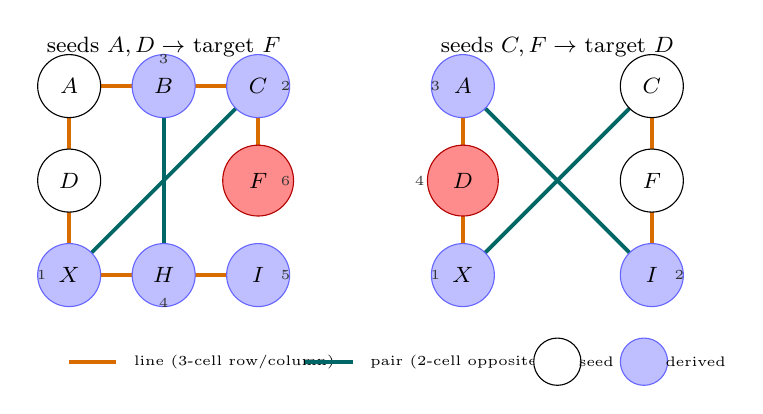
\begin{tikzpicture}[x=1cm, y=1cm, font=\footnotesize,
  seedn/.style={circle, draw, fill=white, minimum size=8mm, inner sep=0pt},
  known/.style={circle, draw=blue!60, fill=blue!25, minimum size=8mm, inner sep=0pt},
  targetn/.style={circle, draw=red!70!black, fill=red!45, minimum size=9mm, inner sep=0pt},
  lineedge/.style={draw=orange!85!black, line width=1.4pt},
  pairedge/.style={draw=teal!80!black, line width=1.4pt},
  ord/.style={font=\tiny, gray!40!black}
]
  % ===== Chain 1: seeds A,D -> target F =====
  \begin{scope}
    \node at (1.2,2.9) {seeds $A,D \to$ target $F$};
    \draw[lineedge] (0,2.4) -- (0,0);       % col1
    \draw[pairedge] (0,0) -- (2.4,2.4);     % pair C,X
    \draw[lineedge] (0,2.4) -- (2.4,2.4);   % row1
    \draw[pairedge] (1.2,2.4) -- (1.2,0);   % pair B,H
    \draw[lineedge] (0,0) -- (2.4,0);       % row3
    \draw[lineedge] (2.4,2.4) -- (2.4,1.2); % col3
    \node[seedn]   (A1) at (0,2.4)   {$A$};
    \node[seedn]   (D1) at (0,1.2)   {$D$};
    \node[known]   (X1) at (0,0)     {$X$};
    \node[known]   (C1) at (2.4,2.4) {$C$};
    \node[known]   (B1) at (1.2,2.4) {$B$};
    \node[known]   (H1) at (1.2,0)   {$H$};
    \node[known]   (I1) at (2.4,0)   {$I$};
    \node[targetn] (F1) at (2.4,1.2) {$F$};
    \node[ord] at (-0.35,0)   {1};
    \node[ord] at (2.75,2.4)  {2};
    \node[ord] at (1.2,2.75)  {3};
    \node[ord] at (1.2,-0.35) {4};
    \node[ord] at (2.75,0)    {5};
    \node[ord] at (2.75,1.2)  {6};
  \end{scope}
  % ===== Chain 2: seeds C,F -> target D =====
  \begin{scope}[shift={(5,0)}]
    \node at (1.2,2.9) {seeds $C,F \to$ target $D$};
    \draw[pairedge] (2.4,2.4) -- (0,0);     % pair C,X
    \draw[lineedge] (2.4,2.4) -- (2.4,0);   % col3
    \draw[pairedge] (0,2.4) -- (2.4,0);     % pair A,I
    \draw[lineedge] (0,2.4) -- (0,0);       % col1
    \node[known]   (X2) at (0,0)     {$X$};
    \node[seedn]   (C2) at (2.4,2.4) {$C$};
    \node[seedn]   (F2) at (2.4,1.2) {$F$};
    \node[known]   (I2) at (2.4,0)   {$I$};
    \node[known]   (A2) at (0,2.4)   {$A$};
    \node[targetn] (D2) at (0,1.2)   {$D$};
    \node[ord] at (-0.35,0)   {1};
    \node[ord] at (2.75,0)    {2};
    \node[ord] at (-0.35,2.4) {3};
    \node[ord] at (-0.55,1.2) {4};
  \end{scope}
  % ===== legend =====
  \begin{scope}[shift={(0,-1.1)}]
    \draw[lineedge] (0,0) -- (0.6,0); \node[right, font=\tiny] at (0.7,0) {line (3-cell row/column)};
    \draw[pairedge] (3.0,0) -- (3.6,0); \node[right, font=\tiny] at (3.7,0) {pair (2-cell opposite)};
    \node[seedn, minimum size=6mm] at (6.2,0) {}; \node[right, font=\tiny] at (6.35,0) {seed};
    \node[known, minimum size=6mm] at (7.3,0) {}; \node[right, font=\tiny] at (7.45,0) {derived};
  \end{scope}
\end{tikzpicture}
\end{center}

\section{Recurrence Across Chains: the Role of $X$}\label{sec:recurrence}

Section~\ref{sec:nestedchains} built one long chain from $A,D,E$,
reaching $F$ through $X,C^2,B^2,H^2,I^2$. Drawn as a dependency graph
on the grid, every step of that chain is a single clean geometric
identity --- none is a combination of two --- which is why the
alternation of Section~\ref{sec:walk} is so regular.

\begin{center}
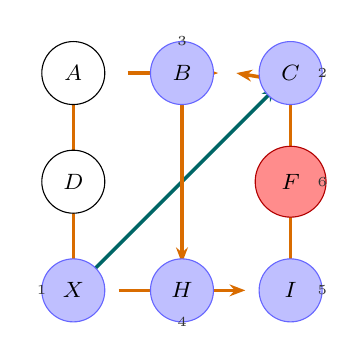
\begin{tikzpicture}[x=1.15cm, y=1.15cm, font=\footnotesize,
  seedn/.style={circle, draw, fill=white, minimum size=8mm, inner sep=0pt},
  known/.style={circle, draw=blue!60, fill=blue!25, minimum size=8mm, inner sep=0pt},
  targetn/.style={circle, draw=red!70!black, fill=red!45, minimum size=9mm, inner sep=0pt},
  lineedge/.style={draw=orange!85!black, line width=1.3pt, -{Stealth[length=2mm]}},
  pairedge/.style={draw=teal!80!black, line width=1.3pt, -{Stealth[length=2mm]}},
  ord/.style={font=\tiny, gray!40!black}
]
  \draw[lineedge] (0,2.4) -- (0,1.3);   \draw[lineedge] (0,1.1) -- (0,0.1);
  \draw[pairedge] (0.15,0.15) -- (2.25,2.25);
  \draw[lineedge] (0.6,2.4) -- (1.6,2.4); \draw[lineedge] (2.4,2.3) -- (1.8,2.4);
  \draw[lineedge] (1.2,2.1) -- (1.2,0.3);
  \draw[lineedge] (0.5,0) -- (1.9,0); \draw[lineedge] (2.4,0) -- (2.4,0);
  \draw[lineedge] (2.4,2.1) -- (2.4,1.3); \draw[lineedge] (2.4,0.1) -- (2.4,1.1);
  \node[seedn]   (A1) at (0,2.4)   {$A$};
  \node[seedn]   (D1) at (0,1.2)   {$D$};
  \node[known]   (X1) at (0,0)     {$X$};   \node[ord] at (-0.35,0)   {1};
  \node[known]   (C1) at (2.4,2.4) {$C$};   \node[ord] at (2.75,2.4)  {2};
  \node[known]   (B1) at (1.2,2.4) {$B$};   \node[ord] at (1.2,2.75)  {3};
  \node[known]   (H1) at (1.2,0)   {$H$};   \node[ord] at (1.2,-0.35) {4};
  \node[known]   (I1) at (2.4,0)   {$I$};   \node[ord] at (2.75,0)    {5};
  \node[targetn] (F1) at (2.4,1.2) {$F$};   \node[ord] at (2.75,1.2)  {6};
\end{tikzpicture}
\end{center}

A second, independent chain, seeded instead by $C,F,E$, reaches $D$
through the same kind of nesting. Solving the six defining equations
for $A^2$ and $X$ in terms
of $C^2,F^2,E^2$ gives $X=2E^2-C^2$ and $A^2=C^2+F^2-E^2$; chaining
forward from there, and using
\[
H^2+I^2 = (E^2+A^2-X)+(2E^2-A^2) = 3E^2-X = A^2+(3E^2-A^2-X) = A^2+D^2 ,
\]
--- itself a direct instance of the redundancy in
Proposition~\ref{prop:rank} --- gives $D^2=H^2+I^2-A^2$ and hence:
\[
\resizebox{0.97\textwidth}{!}{$\displaystyle
D = \left(\left(E^2+\left(C^2+F^2-E^2\right)-\left(2E^2-C^2\right)\right)
+\left(E^2+\left(2E^2-\left(E^2+\left(C^2+F^2-E^2\right)-\left(2E^2-C^2\right)\right)\right)-\left(2E^2-C^2\right)\right)
-\left(C^2+F^2-E^2\right)\right)^{1/2} = 527
$}
\]
Reading it out: $\left(C^2+F^2-E^2\right)$ is $A^2$, $\left(2E^2-C^2\right)$
is $X$, the first large parenthesis is $H^2$, the second is $I^2$, and
$H^2+I^2-A^2$ closes at $D^2$.

Drawn the same way, this chain looks markedly different: most of its
steps combine two prior identities rather than applying one, since
Proposition~\ref{prop:closedform} itself already draws on two of the
square's identities before this chain reuses it further.

\begin{center}
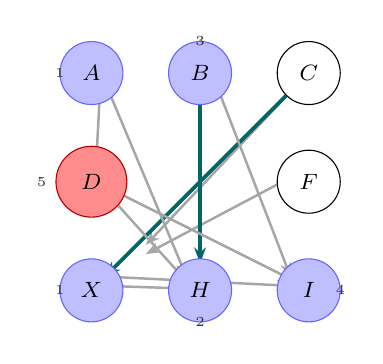
\begin{tikzpicture}[x=1.15cm, y=1.15cm, font=\footnotesize,
  seedn/.style={circle, draw, fill=white, minimum size=8mm, inner sep=0pt},
  known/.style={circle, draw=blue!60, fill=blue!25, minimum size=8mm, inner sep=0pt},
  targetn/.style={circle, draw=red!70!black, fill=red!45, minimum size=9mm, inner sep=0pt},
  pairedge/.style={draw=teal!80!black, line width=1.3pt, -{Stealth[length=2mm]}},
  comedge/.style={draw=black!35, line width=0.9pt, -{Stealth[length=1.8mm]}},
  ord/.style={font=\tiny, gray!40!black}
]
  \draw[comedge] (2.3,2.3) -- (0.6,0.5);
  \draw[comedge] (2.3,1.3) -- (0.6,0.4);
  \draw[pairedge] (2.25,2.25) -- (0.15,0.15);
  \draw[comedge] (0.15,2.3) -- (1.05,0.15);
  \draw[comedge] (0.15,0.05) -- (1.05,0.02);
  \draw[pairedge] (1.2,2.1) -- (1.2,0.3);
  \draw[comedge] (1.35,2.35) -- (2.2,0.15);
  \draw[comedge] (0.2,0.15) -- (2.2,0.05);
  \draw[comedge] (1.05,0.1) -- (0.15,1.1);
  \draw[comedge] (2.25,0.1) -- (0.15,1.15);
  \draw[comedge] (0.1,2.3) -- (0.05,1.35);
  \node[known]   (X2) at (0,0)     {$X$};   \node[ord] at (-0.35,0)   {1};
  \node[seedn]   (C2) at (2.4,2.4) {$C$};
  \node[seedn]   (F2) at (2.4,1.2) {$F$};
  \node[known]   (A2) at (0,2.4)   {$A$};   \node[ord] at (-0.35,2.4) {1};
  \node[known]   (H2) at (1.2,0)   {$H$};   \node[ord] at (1.2,-0.35) {2};
  \node[known]   (B2) at (1.2,2.4) {$B$};   \node[ord] at (1.2,2.75)  {3};
  \node[known]   (I2) at (2.4,0)   {$I$};   \node[ord] at (2.75,0)    {4};
  \node[targetn] (D2) at (0,1.2)   {$D$};   \node[ord] at (-0.55,1.2) {5};
\end{tikzpicture}
\end{center}

Only $C \to X$ and $H \to B$ (teal) are single clean pair identities;
every other arrow (gray) combines two prior quantities at once, and
the final step merges three ($H^2$, $I^2$, and $A^2$) to close at
$D^2$. Eleven dependency edges in all, against the first chain's ten
--- but concentrated into five tiers instead of six, and mostly
combined rather than clean, which is exactly why the shorter,
all-clean four-step route of Section~\ref{sec:walk} is the better path
to $D$.

Comparing the two chains lets a question be asked precisely: which
cell recurs the most as a \emph{derived} quantity, once seeds --- which
cost nothing to reference, since they are simply given --- are excluded
from the count?

\begin{center}
\begin{tabular}{lccc}
\hline
Chain & Seeds & $X$ occurrences & Next-most-recurrent \\
\hline
$A,D,E \to F$ & $A,D,E$ & $3$ & $C^2$: $2$ \\
$C,F,E \to D$ & $C,F,E$ & $3$ & $A^2$: $3$ (tied) \\
\hline
\end{tabular}
\end{center}

In the first chain $X$ recurs more than any other derived quantity; in
the second it ties with $A^2$, which --- unlike in the first chain,
where $A$ is a free seed --- must itself be computed from $C,F,E$
before it can be reused at all. The precise statement is not that $X$
is the unique recurring cell, but that it is never surpassed: across
two independent choices of seed pair, $X$ recurs at least as often as
anything else derived, tying at worst. This follows from
Proposition~\ref{prop:rank}: $\{A^2,E^2,X\}$ is the three-parameter
basis underlying all six defining equations
\eqref{eq:C}--\eqref{eq:F}, so $X$ --- together with whichever cell
plays $A^2$'s role in a given chain --- is structurally load-bearing
for every other cell, appearing in five of the six defining relations.

This structural centrality is distinct from, though complementary to,
a second and separate asymmetry recorded in
Section~\ref{sec:closedform}: swapping which of two representation-list
values is called $A$ and which $D$ changes the outcome, since
$H^2=E^2+A^2-X$ treats $A$ and $D$ unequally --- $(A,D)=(205,527)$
reaches seven squares, while $(A,D)=(527,205)$ reaches only six. That
asymmetry is geometric, arising from $A$ occupying the top-left corner
(shared by the top row, the main diagonal, and the first column) while
$D$ occupies only the middle-left edge (shared by the middle row and
the first column); it is unrelated to $X$'s algebraic centrality, and
neither fact explains the other.

\begin{remark}
It is fair, in this light, to speak informally of $A$ as the cell whose
\emph{position} forces an asymmetric start --- which of two candidate
values is placed there changes the count --- and of $X$ as the cell
that recurs throughout the computation, never less than any other
derived quantity. Both are true statements about this square, arrived
at independently; neither is the cause of the other. In particular,
the outcome that $C$ turns out square while $X$ does not
(Section~\ref{sec:unsimplified}) is settled by $X$'s value the moment
it is first computed --- from $C^2$ alone, or from $A^2+D^2$, whichever
chain one is following --- and not by anything that happens to $X$
later in a chain that goes on to reuse it.
\end{remark}

\section{A Catalog of Chain Shapes}\label{sec:catalog}

Sections~\ref{sec:nestedchains}, \ref{sec:walk}, and \ref{sec:recurrence}
each built a nested-radical chain reaching one target cell from one
seed pair. Collected together, in terms of $E^2$ and the two seeds
alone, the chains found for the square of Section~\ref{sec:ex} are:

\subsection*{Seeded by $A, D, E$}

\[
H = \sqrt{\,2E^2 - \Bigl(3E^2-A^2-\bigl(2E^2-(3E^2-A^2-D^2)\bigr)\Bigr)\,}
  = 23 .
\]
\[
I = \sqrt{\,(A^2+D^2) - \Bigl(2E^2 - \bigl(3E^2-A^2-(2E^2-(3E^2-A^2-D^2))\bigr)\Bigr)\,}
  = 565 .
\]
\[
F = \sqrt{\,\bigl(3E^2-(2E^2-A^2)\bigr) - \bigl(2E^2-(3E^2-A^2-D^2)\bigr)\,}
  = 289 .
\]
The full seven-layer chain to $F$ that instead routes through $C^2$
and $I^2$ both fully expanded is given in
Section~\ref{sec:nestedchains}.

\subsection*{Seeded by $C, F, E$}

\[
X = 2E^2-C^2 = 222121, \qquad I = \sqrt{\,3E^2-C^2-F^2\,} = 565 ,
\]
\[
A = \sqrt{\,2E^2-(3E^2-C^2-F^2)\,} = 205 .
\]
\[
\resizebox{0.9\textwidth}{!}{$\displaystyle
D = \sqrt{\,3E^2 - \bigl(2E^2-(3E^2-C^2-F^2)\bigr) - (2E^2-C^2)\,} = 527
$}
\]
\[
\resizebox{0.9\textwidth}{!}{$\displaystyle
B = \sqrt{\,2E^2 - \Bigl(E^2+(C^2+F^2-E^2)-(2E^2-C^2)\Bigr)\,}
  = 600.6005328002965\ldots
$}
\]
\[
\resizebox{0.95\textwidth}{!}{$\displaystyle
I = \sqrt{\,E^2 + \Bigl(2E^2-\bigl(E^2+(C^2+F^2-E^2)-(2E^2-C^2)\bigr)\Bigr) - (2E^2-C^2)\,}
  = 565
$}
\]
The four-step chain above for $D$ is the clean route of
Section~\ref{sec:walk}; the six-layer chain of Section~\ref{sec:recurrence},
which instead passes through $H^2$ and $B^2$, reaches the same $D$ by
a longer, mostly-combined path. The last line recovers $I$ a second
way, reusing the $B$-chain rather than the direct pair identity
$I^2=2E^2-A^2$ --- the same value, $565$, by three independent routes
now on record: directly from $A^2$, via the $A,D,E$ chain above, and
via this $B$-chain.

\begin{center}
\begin{tabular}{llcl}
\hline
Seeds & Target & Layers & Note \\
\hline
$A,D,E$ & $H$ & $4$ & shortest route to $H$ \\
$A,D,E$ & $I$ & $5$ & reuses the $H$-chain \\
$A,D,E$ & $F$ & $3$ & shortest route to $F$ \\
$A,D,E$ & $F$ & $7$ & Section~\ref{sec:nestedchains}, fully expanded \\
$C,F,E$ & $X,I,A$ & $1$--$2$ & direct, no chaining needed \\
$C,F,E$ & $D$ & $4$ & Section~\ref{sec:walk}, all-clean \\
$C,F,E$ & $D$ & $6$ & Section~\ref{sec:recurrence}, mixed \\
$C,F,E$ & $B$ & $4$ & \\
$C,F,E$ & $I$ & $5$ & third route to $I$ \\
\hline
\end{tabular}
\end{center}

\begin{remark}
Every entry in this catalog is guaranteed, by
Proposition~\ref{prop:chaincollapse}, to reduce to one of the six
defining equations \eqref{eq:C}--\eqref{eq:F} however long it is
written --- the table records how many layers of substitution a
particular choice of route happens to take, not a fact about the cell
reached. That several distinct chains reach the same value ($565$ for
$I$, by three separate routes above) is exactly what rank $6$
predicts: with only three free parameters, most quantities of interest
admit more than one path to the same answer.
\end{remark}

\subsection*{The remaining seed pairs}

Twelve pairs of outer cells are valid seeds: any two cells sharing a
row or column, excluding the four opposite pairs
$(A,I),(B,H),(C,X),(D,F)$, which are never independent. They fall into
four families, one per outer line, and $A,D,E \to F$
(Sections~\ref{sec:nestedchains}, \ref{sec:walk}) and
$C,F,E \to D$ (Section~\ref{sec:walk}) already cover two of the four.
A deep, single-thread walk exists for each of the remaining two
families as well.

\paragraph{Row 1: $(A,B)$, $(A,C)$, $(B,C)$.} Represented by $(A,C)$,
reaching $F$:
\[
B^2 = 3E^2-A^2-C^2, \quad I^2=2E^2-A^2, \quad H^2=2E^2-B^2,
\]
\[
X=2E^2-C^2, \quad D^2=3E^2-A^2-X,
\]
\[
F^2 = 3E^2-C^2-I^2 = 83521, \qquad F = 289 .
\]
$(A,B)$ and $(B,C)$ reach the same six values by the same identities,
after one preliminary step to recover the missing row-1 member:
$C^2=3E^2-A^2-B^2$ for $(A,B)$, or $A^2=3E^2-B^2-C^2$ for $(B,C)$.

\paragraph{Row 3: $(X,H)$, $(X,I)$, $(H,I)$.} Represented by $(H,I)$,
reaching $F$:
\[
X = 3E^2-H^2-I^2, \quad A^2=2E^2-I^2, \quad B^2=2E^2-H^2, \quad
C^2=2E^2-X, \quad D^2=3E^2-A^2-X,
\]
\[
F^2 = 3E^2-C^2-I^2 = 83521, \qquad F = 289 .
\]
$(X,H)$ and $(X,I)$ reach the same six values after recovering the
missing row-3 member: $I^2=3E^2-X-H^2$ for $(X,H)$, or
$H^2=3E^2-X-I^2$ for $(X,I)$.

\paragraph{Column 1: $(A,D)$, $(A,X)$, $(D,X)$.} $(A,D)$ is
Sections~\ref{sec:nestedchains}--\ref{sec:walk}. Represented instead
by $(A,X)$, reaching $H$:
\[
D^2 = 3E^2-A^2-X, \quad I^2=2E^2-A^2, \quad C^2=2E^2-X,
\]
\[
F^2=2E^2-D^2, \quad B^2=3E^2-A^2-C^2,
\]
\[
H^2 = 3E^2-X-I^2 = 529, \qquad H = 23 .
\]
$(D,X)$ reaches the same six values after $A^2=3E^2-D^2-X$ (column 1).

\paragraph{Column 3: $(C,F)$, $(C,I)$, $(F,I)$.} $(C,F)$ is
Section~\ref{sec:walk}. Represented instead by $(C,I)$, reaching $H$:
\[
F^2 = 3E^2-C^2-I^2, \quad A^2=2E^2-I^2, \quad X=2E^2-C^2,
\]
\[
D^2=2E^2-F^2, \quad B^2=3E^2-A^2-C^2,
\]
\[
H^2 = 3E^2-X-I^2 = 529, \qquad H = 23 .
\]
$(F,I)$ reaches the same six values after $C^2=3E^2-F^2-I^2$
(column 3).

\begin{remark}[The shallow alternative]
Every one of these twelve deep walks is optional. Once any single step
produces $X$ (equivalently $C^2$), the remaining five cells follow at
once, in parallel, directly from \eqref{eq:C}--\eqref{eq:F} applied to
$A^2$, $X$, and $E^2$ --- two steps in total from any seed pair, not
six. The six-step walks above are deliberately the longer route,
chosen because each of their steps is individually a clean geometric
identity, tracing the square rather than shortcutting through it. As
with the chain (II1)--(II6) of Section~\ref{sec:11E}, the number of
layers records a choice of path, not a property of the cell reached; a
fuller account of what the shallow path says about $X$ itself is taken
up in a later section.
\end{remark}

\section{The Anchor Basis and the Parity of the Elimination Chain}\label{sec:anchorparity}

Three separate constructions --- the elimination chain
(II1)--(II6) of Section~\ref{sec:11E}, the deep walks of
Sections~\ref{sec:nestedchains}--\ref{sec:catalog}, and the shallow
alternative of Section~\ref{sec:catalog} --- converge on the same
destination, and doing so is not a coincidence but a consequence of
rank.

\begin{proposition}\label{prop:tripleE}
Every relation expressing one cell as $E^2$ plus or minus exactly two
other cells --- a \emph{triple} relation --- uses $E^2$ with
coefficient $1$, never $2E^2$.
\end{proposition}

\begin{proof}
The four anchor forms of Section~\ref{sec:anchors},
\[
B^2=-E^2+I^2+X, \qquad D^2=E^2+I^2-X, \qquad F^2=E^2-I^2+X, \qquad
H^2=E^2+A^2-X ,
\]
already exhibit this. Any further triple relation is a rearrangement
of one of these or of \eqref{eq:C}--\eqref{eq:F}: for instance
$A^2=E^2+C^2-D^2$ (from column 1 combined with the corner pair) and
$A^2=E^2+X-B^2$ (equation~\eqref{eq:B} rearranged) both hold, and both
carry $E^2$ at coefficient $1$. A relation with $2E^2$ instead would
require two independent applications of Corollary~\ref{cor:pairs}
within a single triple, which needs four outer cells, not two, to
balance.
\end{proof}

\begin{remark}
Among the four triples above, $X$ is not merely present in some: it is
present in \emph{all four}, alternating sign
($+X,-X,+X,-X$) as the cell cycles through $B,D,F,H$. The partner term
alternates too, but in a different pattern --- $I^2$ for $B,D,F$, since
these are exactly the three vertices of the medial triangle around the
anchors $\{I^2,X\}$ (the Medial configuration of
Section~\ref{sec:anchors}), and $A^2$ for $H$, which sits outside that
triangle as $B$'s opposite-pair partner rather than a medial vertex.
No triple relation among $B,D,F,H$ omits $X$; each omits $I^2$ or
$A^2$ instead. This is the precise sense in which $X$ is unavoidable
for these four cells specifically, and it is independent of, though
consistent with, its role as the shared floor of
Proposition~\ref{prop:parity11}.
\end{remark}

\begin{proposition}\label{prop:parity11}
The constants $11,9,7,5,3,1$ of (II1)--(II6) are all odd, and no
relation in that chain, extended in either direction, can close at an
even multiple of $E^2$.
\end{proposition}

\begin{proof}
Rearranged, (II6) reads $B^2=-E^2+I^2+X$, which is exactly the anchor
form above: coefficient $1$, odd. Each subsequent step of the chain,
by Section~\ref{sec:11E}, trades one cell for its opposite-pair
partner via Corollary~\ref{cor:pairs}, changing the constant by
exactly $2E^2$. Starting from an odd coefficient and moving by even
steps preserves parity indefinitely, so every constant reachable from
(II6) --- in particular the observed $1,3,5,7,9,11$ --- is odd.
$12E^2$, or any even multiple, is therefore not merely absent from the
six relations recorded: it is structurally unreachable by this chain,
regardless of how far the elimination is extended.
\end{proof}

The anchor forms are the natural terminus of this descent because
$\{E^2,I^2,X\}$ (Section~\ref{sec:anchors}) is already a minimal
three-parameter basis: no further substitution can reduce a triple
relation past coefficient $1$, since doing so would require
eliminating a fourth free quantity from a system that only has three.
This is the same basis the shallow alternative of
Section~\ref{sec:catalog} reaches after two steps from \emph{any} seed
pair, and the same pair $\{X,A^2\}$ (or $\{X,I^2\}$) that dominates the
recurrence counts of Section~\ref{sec:recurrence}. The elimination
chain descends toward it from above by removing pairs two at a time;
the deep walks approach it from below by adding lines and pairs one at
a time; the shallow alternative reaches it directly. All three are
different routes to the identical resting point.

\begin{remark}
This sharpens, without overclaiming, the informal claim that $X$
``closes'' the square. $X$ is not closing in every literal sense ---
it is itself a valid seed in four of the twelve pairs of
Section~\ref{sec:catalog}, where it costs nothing to reference --- but
it is never more than one step from a seed pair that does not include
it, and together with $A^2$ (or $I^2$) it is the fixed basis that
every elimination, deep or shallow, is forced back toward. The
elimination chain's confinement to odd multiples of $E^2$ is the
precise, provable form of that fact: not that $X$ is privileged over
every other cell, but that the basis $\{E^2,I^2,X\}$ it belongs to is
the unique floor beneath which no further reduction, by any route, is
possible.
\end{remark}

\section{$X$ as the Closing Cell}\label{sec:xclosing}

The term \emph{closing cell} was introduced in Section~\ref{sec:ex} in
a narrow, search-specific sense: once $A$ and $C$ are chosen so that
$A^2$ and $C^2$ are square, $X$ and $B^2$ are the two entries left
over, fixed by the linear structure regardless of whether they
themselves are square. Three independent lines of evidence, developed
since, show that $X$ closes the square in a second, purely algebraic
sense as well --- not tied to any particular search, and not a
property of which two cells happen to be chosen as seeds.

\paragraph{In the chains.} Section~\ref{sec:recurrence} compared two
independently seeded deep chains and found that $X$, once it must be
derived rather than handed over as a seed, recurs at least as often as
any other derived quantity --- outright in one chain, tied with $A^2$
in the other, never surpassed. Section~\ref{sec:catalog} then showed
that this is not particular to those two chains: of the twelve valid
seed pairs, every deep walk passes through $X$ at some point, and the
shallow alternative available to all twelve reaches $X$ (or already
has it, when $X$ is itself a seed) within a single step, after which
every remaining cell follows in parallel.

\paragraph{In the $E^2$ relations.} Proposition~\ref{prop:tripleE} and
the remark following it show that among the four triples
$B^2,D^2,F^2,H^2$ --- the minimal, single-$E^2$ expressions for the
four edge cells --- $X$ appears in \emph{all four}, alternating sign,
while its partner term alternates between $I^2$ and $A^2$. No minimal
relation among these four cells omits $X$; each omits one of the two
corner anchors instead.

\paragraph{In (II1)--(II6).} $X$ is not only the subject of the entire
elimination chain of Section~\ref{sec:11E}, appearing on both sides of
(II1); Proposition~\ref{prop:parity11} shows the chain's confinement
to odd multiples of $E^2$ is inherited directly from $X$'s presence
in the anchor form at (II6), the chain's terminus. Every relation the
chain passes through on its way from $11E^2$ down to $E^2$ is, in
effect, a restatement of where $X$ sits relative to the other eight
cells.

\begin{center}
\begin{tabular}{lp{9.5cm}}
\hline
Evidence & What it shows \\
\hline
Chains (\ref{sec:recurrence}, \ref{sec:catalog}) & $X$ recurs at least
as often as any derived quantity, across every seed pair tested, and
is at most one step away when not itself a seed. \\
Triples (\ref{sec:anchorparity}) & $X$ appears in all four minimal
edge-cell relations; none omits it. \\
(II1)--(II6) (\ref{sec:11E}, \ref{sec:anchorparity}) & The chain is
built on $X$ throughout, and its odd-only parity is forced by $X$'s
role in the anchor form at the chain's end. \\
\hline
\end{tabular}
\end{center}

A single argument, from degrees of freedom alone, accounts for all
three lines of evidence at once.

\begin{proposition}\label{prop:xindispensable}
Fix $A$ and its opposite-pair partner $I$ (so $A^2+I^2=2E^2$). No cell
among $B^2,C^2,D^2,F^2,H^2$ is determined by $A^2$, $I^2$, and $E^2$
alone; each requires $X$ as well.
\end{proposition}

\begin{proof}
Since $A^2+I^2=2E^2$, the pair $(A^2,I^2)$ carries only one free
number beyond $E^2$, not two. Proposition~\ref{prop:rank} requires
exactly three free parameters to determine the family. One of the
three is E$^2$ itself; a second is spent on $A^2$ (with $I^2$ fixed by
it); a third remains unspent, and no relation among
\eqref{eq:C}--\eqref{eq:F} can produce a fifth cell from only two free
numbers. $X$ is exactly the missing third parameter --- indeed the
same $X$ of Proposition~\ref{prop:rank}'s own basis $\{A^2,E^2,X\}$ ---
and every one of $B^2,C^2,D^2,F^2,H^2$ requires it:
\[
B^2=-E^2+I^2+X, \quad D^2=E^2+I^2-X, \quad F^2=E^2-I^2+X,
\]
\[
H^2=E^2+A^2-X, \qquad C^2=2E^2-X .
\]
\end{proof}

Unlike the triples of Proposition~\ref{prop:tripleE}, this is not
restricted to $B,D,F,H$: it is a statement about the whole square,
and it includes $C^2$ directly through its own simplest relation
rather than through any longer detour. The apparent tension with
Proposition~\ref{prop:tripleE}'s remark --- that $A^2=E^2+C^2-D^2$ is
a valid $X$-free triple --- is resolved by what that triple actually
uses: $D^2$, a cell outside the closed vocabulary $\{A^2,I^2,E^2,X\}$
of Proposition~\ref{prop:xindispensable}. Within that vocabulary, $X$
is not optional for any of the five remaining cells; escaping it
requires importing a sixth quantity from outside, which is a different
and more expensive kind of route, not a shorter one.

\begin{remark}
This is the precise and provable form of the informal claim that $X$
closes the square starting from any single seed $A$: fix $A$, and its
opposite pair $I$ follows for free, but nothing else does without $X$.
None of this makes $X$ more important than $A^2$ in an absolute sense
--- Section~\ref{sec:recurrence} already established that $A^2$ ties
$X$'s recurrence when it, too, must be derived, and
$\{A^2,E^2,X\}$ is a basis of three, not one. What
Proposition~\ref{prop:xindispensable} shows is narrower and more
precise: of the three free parameters the family needs, one is always
spent on $E^2$ and the natural second is spent on the pair $(A,I)$
--- and whichever cell is asked to supply the third, within that
closed vocabulary it can only be $X$. That is the algebraic content
behind calling $X$ a closing cell, alongside its original, narrower
meaning from Section~\ref{sec:ex}.
\end{remark}

\begin{remark}
Stated at its simplest: fixing $E$ leaves exactly two degrees of
freedom. Choosing the seed $A$ spends the first, and fixes $I$ with it
at no extra cost, via $A^2+I^2=2E^2$. That leaves exactly one degree
of freedom unspent, and $B^2,C^2,D^2,F^2,H^2$ --- all five of the
remaining cells --- are reached only by spending it on $X$, each
through nothing more than $\pm E^2$ and $\pm X$ together with the
already-known $A^2$ or $I^2$. There is no other way to spend the
second degree of freedom that reaches any of the five; $X$ is not one
option among several for closing the square in this framework, it is
the only one, and it is the one term shared by all five closing
equations alike.
\end{remark}

\section{The Sign Signature $(+1,-1)$ and Adjacency to $X$}\label{sec:signature}

With $E$ fixed and the seed $A$ spending the first degree of freedom
(fixing $I$ for free, Proposition~\ref{prop:xindispensable}), the
second and only remaining degree of freedom is $X$. The sign each
cell's coefficient-$1$ relation carries on $E^2$ and $X$ is not
arbitrary: it identifies precisely how the cell sits relative to $X$
on the grid, and whether that placement is forced or merely one choice
among two.

\begin{proposition}[The $X$-sign rule]\label{prop:xsign}
A cell's minimal relation carries $-X$ if it shares a row, column, or
the corner opposite pair with $X$ directly; it carries $+X$ if it is
instead the opposite-pair partner of such a cell.
\end{proposition}

\begin{proof}
$D$ shares column 1 with $X$ ($A^2+D^2+X=3E^2$); $H$ shares row 3 with
$X$ ($X+H^2+I^2=3E^2$); $C$ is $X$'s own opposite pair
(Corollary~\ref{cor:pairs}). Solving each of these three identities
for the cell in question produces $-X$ directly. $B$ and $F$ share no
line with $X$ and are not paired with it; they are instead the
opposite-pair partners of $H$ and $D$ respectively, and
$\mathrm{partner}^2=2E^2-\mathrm{cell}^2$ negates every term of the
partner's own equation, turning $H$'s $-X$ into $B$'s $+X$, and $D$'s
$-X$ into $F$'s $+X$.
\end{proof}

\begin{proposition}[Forced vs.\ free sign]\label{prop:esign}
Among the coefficient-$1$ triples for $B^2,D^2,F^2,H^2$: $D^2$ and
$H^2$ admit exactly one sign assignment of $E^2$, together with $I^2$
or $A^2$ respectively; $B^2$ and $F^2$ admit two, one using $A^2$ and
one using $I^2$, differing in the sign of $E^2$.
\end{proposition}

\begin{proof}
Exhaustive search over $s_1 E^2 + s_2\{A^2 \text{ or } I^2\} + s_3 X$,
$s_i\in\{+1,-1\}$, against the known numerical values finds exactly
one solution for $D^2$, using $I^2$, and none using $A^2$; exactly one
for $H^2$, using $A^2$, and none using $I^2$; and, for each of
$B^2,F^2$, one solution using $A^2$ and a second, distinct, using
$I^2$:
\[
D^2=E^2+I^2-X, \qquad H^2=E^2+A^2-X,
\]
\[
B^2=E^2-A^2+X=-E^2+I^2+X, \qquad F^2=-E^2+A^2+X=E^2-I^2+X .
\]
\end{proof}

Combined, this identifies a genuine geometric signature. $D,H,C$ ---
the three cells directly adjacent to $X$, by line or by pair --- are
forced into the single sign pattern $(E^2,X)=(+1,-1)$ (for $C$,
doubled: $C^2=E^2+E^2-X$), with no alternative available. $B,F$ ---
reached only by stepping through an opposite-pair flip --- are not
forced: each admits two valid coefficient-$1$ forms, $(+1,+1)$ using
its own natural anchor or $(-1,+1)$ using the translated one, and it
is exactly this freedom that marks them as one step removed from $X$
rather than directly adjacent to it.

\begin{center}
\begin{tabular}{lccl}
\hline
Cell & Adjacent to $X$? & $(E^2,X)$ sign & Forced? \\
\hline
$D$ & column 1 & $(+1,-1)$ & yes, unique \\
$H$ & row 3 & $(+1,-1)$ & yes, unique \\
$C$ & opposite pair & $(+1,-1)$ & yes, unique \\
$B$ & no (partner of $H$) & $(+1,+1)$ or $(-1,+1)$ & no, two forms \\
$F$ & no (partner of $D$) & $(+1,+1)$ or $(-1,+1)$ & no, two forms \\
\hline
\end{tabular}
\end{center}

\begin{remark}
The sign pattern is therefore diagnostic, not incidental: given any
coefficient-$1$ triple for one of the five remaining cells, whether
its $(E^2,X)$ signs are forced to $(+1,-1)$ or free to be either
$(+1,+1)$ or $(-1,+1)$ reveals, without consulting the grid at all,
whether that cell sits directly on a line or pair with $X$ or one step
away from it. Searching for the signature $(+1,-1)$ is, in this
precise sense, searching for the specific geometric formation of
direct adjacency to $X$ --- and Proposition~\ref{prop:xsign} guarantees
the search succeeds for exactly three of the five, never more and
never fewer.
\end{remark}

\section{Unique Formation for $D, H, C$}\label{sec:formationnote}

Fixing $A$, $E$, and $X$ determines every cell of the square uniquely
--- Proposition~\ref{prop:param} allows no other outcome. It is
tempting to extend that uniqueness to the sign formation each cell is
written in, but Proposition~\ref{prop:esign} already shows this is
false for two of the five remaining cells, and the distinction is
worth keeping sharp rather than rounding away.

\begin{itemize}
\item \textbf{Values are always unique.} For any $A,E,X$, each of
$B^2,C^2,D^2,F^2,H^2$ takes exactly one value, with no ambiguity.
\item \textbf{Formations are unique only for $D,H,C$.} Each of these
three has exactly one valid sign template at coefficient $1$
(Proposition~\ref{prop:esign}): once $A,E,X$ are fixed, no second
formation matches.
\item \textbf{Formations are two-way for $B,F$.} Each of these two has
\emph{two} valid sign templates --- one per corner anchor --- and both
correctly reach the same value. Neither formation is privileged over
the other; both match simultaneously.
\end{itemize}

So it is not correct to say that fixing $A,E,X$ creates a single
formation that no other can match, in full generality: that statement
is exactly right for $D,H,C$, and exactly wrong for $B,F$, whose
defining feature is precisely that two formations tie. The asymmetry
is the result, not an exception to it: it is what separates the three
cells directly adjacent to $X$ (Proposition~\ref{prop:xsign}) from the
two reached only through an opposite-pair flip, and collapsing it
into a single blanket claim of uniqueness would erase the distinction
Section~\ref{sec:signature} was built to establish.

\section{The $(C,E,X)$ Reflection and the Three-Panel View}\label{sec:reflection}

The mirrored placements in the sign panels are not incidental: they
are the trace of a single symmetry of the square, the reflection
across the diagonal through $C$, $E$, $X$.

\begin{proposition}\label{prop:cexreflection}
Reflecting the square across the diagonal $C,E,X$ fixes $C$, $E$, and
$X$, and swaps $A\leftrightarrow I$, $B\leftrightarrow F$, and
$D\leftrightarrow H$.
\end{proposition}

\begin{proof}
This is one of the eight symmetries of Section~\ref{sec:rotation}
(``Symmetries of the square''), the reflection through the anti-diagonal
$C,E,X$ rather than the main diagonal $A,E,I$ used there as the
illustrative rotation. Written as $(i,j)\mapsto(4-j,4-i)$ on the grid
coordinates, it fixes exactly the three cells on that diagonal and
exchanges each remaining cell with the one occupying the mirrored
position: $A$ (top-left) with $I$ (bottom-right), $B$ (top-middle)
with $F$ (middle-right), $D$ (middle-left) with $H$ (bottom-middle).
\end{proof}

Applying the swap $A^2\leftrightarrow I^2$ together with
$B\leftrightarrow F$ to the sign forms of
Section~\ref{sec:signature} carries one exactly onto the other:
\[
B^2=E^2-A^2+X \ \xrightarrow{\ A^2\leftrightarrow I^2,\ B\leftrightarrow F\ }\ F^2=E^2-I^2+X ,
\]
\[
B^2=-E^2+I^2+X \ \xrightarrow{\ A^2\leftrightarrow I^2,\ B\leftrightarrow F\ }\ F^2=-E^2+A^2+X ,
\]
and the same swap, applied to $D\leftrightarrow H$, carries $D$'s
single forced form onto $H$'s:
\[
D^2=E^2+I^2-X \ \xrightarrow{\ A^2\leftrightarrow I^2,\ D\leftrightarrow H\ }\ H^2=E^2+A^2-X .
\]
The three panels below display exactly this: each plots two of
$A^2,I^2,X$ against $E^2$, and the reflection of
Proposition~\ref{prop:cexreflection} is the map that carries every
label to its mirror image across the origin.

\begin{center}
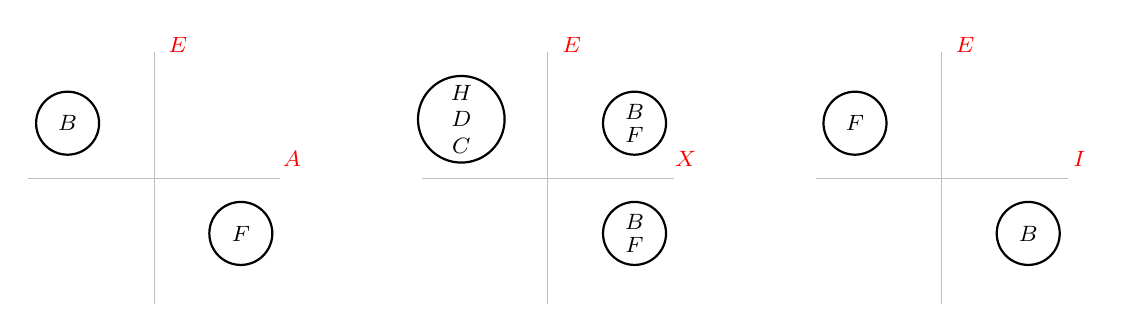
\begin{tikzpicture}[x=1cm,y=1cm,font=\footnotesize]
  % Panel 1: (A,E) plane
  \begin{scope}
    \draw[gray!50] (-1.6,0) -- (1.6,0);
    \draw[gray!50] (0,-1.6) -- (0,1.6);
    \node[red] at (1.75,0.25) {$A$};
    \node[red] at (0.3,1.7) {$E$};
    \draw[thick] (-1.1,0.7) circle (0.4); \node at (-1.1,0.7) {$B$};
    \draw[thick] (1.1,-0.7) circle (0.4); \node at (1.1,-0.7) {$F$};
  \end{scope}
  % Panel 2: (X,E) plane
  \begin{scope}[shift={(5,0)}]
    \draw[gray!50] (-1.6,0) -- (1.6,0);
    \draw[gray!50] (0,-1.6) -- (0,1.6);
    \node[red] at (1.75,0.25) {$X$};
    \node[red] at (0.3,1.7) {$E$};
    \draw[thick] (-1.1,0.75) circle (0.55);
    \node[align=center] at (-1.1,0.75) {$H$\\$D$\\$C$};
    \draw[thick] (1.1,0.7) circle (0.4); \node at (1.1,0.7) {\shortstack{$B$\\$F$}};
    \draw[thick] (1.1,-0.7) circle (0.4); \node at (1.1,-0.7) {\shortstack{$B$\\$F$}};
  \end{scope}
  % Panel 3: (I,E) plane
  \begin{scope}[shift={(10,0)}]
    \draw[gray!50] (-1.6,0) -- (1.6,0);
    \draw[gray!50] (0,-1.6) -- (0,1.6);
    \node[red] at (1.75,0.25) {$I$};
    \node[red] at (0.3,1.7) {$E$};
    \draw[thick] (-1.1,0.7) circle (0.4); \node at (-1.1,0.7) {$F$};
    \draw[thick] (1.1,-0.7) circle (0.4); \node at (1.1,-0.7) {$B$};
  \end{scope}
\end{tikzpicture}
\end{center}

\begin{remark}
The reflection accounts for the mirroring visible across all three
panels --- it is the single symmetry that carries $B$'s two forms onto
$F$'s two forms, and $D$'s one form onto $H$'s one form, all at once
--- but it does not by itself explain why $B,F$ have two forms while
$D,H,C$ have only one. That asymmetry is fixed by the reflection, not
produced by it: $C$ and $X$ lie on the mirror line, so their direct
adjacency to $X$ (Proposition~\ref{prop:xsign}) is preserved rather
than exchanged, while $A\leftrightarrow I$ and $B\leftrightarrow F$
are genuinely swapped. The unique formation of $D,H,C$ and the
two-way formation of $B,F$ (Section~\ref{sec:formationnote}) are each
individually preserved by this symmetry; the reflection relates the
two halves of the free pair to each other, but the reason one pair is
free and the other is not remains the adjacency argument, established
independently of any rotation or reflection of the square.
\end{remark}

\section{Unique Formation for the Seed $A$ and Scale $E$}\label{sec:uniqueformation}

Proposition~\ref{prop:cexreflection} showed that the full reflection
across $C,E,X$ preserves every line of the square. It is worth
checking directly that no smaller, partial rearrangement does the
same --- so that the reflection is not merely \emph{a} symmetry that
happens to work, but the only available move once $A$ and $E$ are
fixed.

\begin{proposition}\label{prop:nopartial}
Once $A$ and $E$ are fixed, no partial swap of cells --- exchanging a
single opposite pair in isolation, or exchanging two cells that are
not an opposite pair --- preserves all eight lines of the square.
Only the full reflection of Proposition~\ref{prop:cexreflection},
moving $A,I,B,F,D,H$ together, does.
\end{proposition}

\begin{proof}
Consider the square of Section~\ref{sec:ex}. Swapping the opposite
pair $B^2\leftrightarrow H^2$ alone leaves column 2 (their shared
line) correct, since it contains both and addition does not see their
order:
\[
B^2+E^2+H^2 = H^2+E^2+B^2 .
\]
But $B$ also lies in row 1 and $H$ also lies in row 3, and neither
line contains the other cell of the pair:
\[
A^2+H^2+C^2 = 181683 \ne 3E^2, \qquad X+B^2+I^2 = 902067 \ne 3E^2 .
\]
The identical argument applies to the opposite pair
$D^2\leftrightarrow F^2$, via column 1 and column 3, and to the bare
exchange $B^2\leftrightarrow F^2$ (not an opposite pair at all), which
fails row 1 and row 2 immediately. In every partial case, the swapped
cells' \emph{shared} line survives by commutativity, while at least
one \emph{other} line, containing only one member of the swap, does
not. The full reflection avoids this because it moves every affected
cell at once: substituting $A\!\leftrightarrow\! I$,
$B\!\leftrightarrow\! F$, $D\!\leftrightarrow\! H$ simultaneously
into all eight lines verifies each one directly.
\end{proof}

\begin{center}
\begin{tabular}{lccc}
\hline
Swap attempted & Shared line & Other lines & Valid? \\
\hline
$B^2\leftrightarrow H^2$ alone & column 2: holds & row 1, row 3: fail & no \\
$D^2\leftrightarrow F^2$ alone & row 2: holds & column 1, column 3: fail & no \\
$B^2\leftrightarrow F^2$ alone & (not paired) & row 1, row 2: fail & no \\
full $(C,E,X)$ reflection & --- & all eight: hold & yes \\
\hline
\end{tabular}
\end{center}

\begin{remark}[The last-digit square]
Since every odd square ends in $1$, $5$, or $9$
(Section~\ref{sec:signature}), and since reducing an identity modulo
$10$ preserves it, the eight line-sums of the square survive intact
when every cell is replaced by its last digit. For the square of
Section~\ref{sec:ex}:
\[
\begin{array}{|c|c|c|}
\hline
5 & 1 & 9 \\ \hline
9 & 5 & 1 \\ \hline
1 & 9 & 5 \\ \hline
\end{array}
\]
Every row, column, and diagonal --- including the degenerate diagonal
$5+5+5$ --- sums to $15$, matching $3E^2=541875\equiv5\pmod{10}$. This
is not a coincidence restricted to the full values: it is the same
identity, viewed mod $10$, and consequently the same rigidity applies.
Each partial swap of Proposition~\ref{prop:nopartial} that breaks a
real line breaks the corresponding digit line identically --- exchanging
$B,H$ leaves the shared digit column correct but unbalances the two
digit rows containing $A,C$ and $X,I$ --- so the last-digit square is
exactly as resistant to partial rearrangement as the square of squares
itself, for the same structural reason.
\end{remark}

\begin{remark}[Constant digit grids have two causes]
The digit square of Section~\ref{sec:ex}'s example varies across
$\{1,5,9\}$, but a \emph{constant} last-digit grid --- every cell
ending in the same digit --- is also possible, and it is important not
to read this as always signalling the trivial constant square of
Section~\ref{sec:11E}. It arises in two structurally different ways.
\begin{itemize}
\item \textbf{Degenerate:} every cell equals the same value $t$
(Section~\ref{sec:11E}), so every last digit is trivially identical.
Here the digit square is constant because the square itself is
constant.
\item \textbf{Non-degenerate:} the six clean cells of the
$E=1105$ example, $A=455,\,D=1445,\,F=595,\,H=245,\,I=1495,\,E=1105$,
are six \emph{distinct} numbers, yet each ends in $5$, because each is
divisible by $5$ --- inherited from $1105=5\cdot13\cdot17$ --- and any
odd multiple of $5$ ends in $5$, not $0$. Squaring preserves this, so
every one of these genuinely different cells lands on the same last
digit without any two of them being equal.
\end{itemize}
A constant digit grid is therefore not, by itself, evidence of the
degenerate solution: it can equally well reflect a shared prime factor
inherited from $E$. The reliable signature of degeneracy is constant
\emph{value}, not constant \emph{digit}; the two coincide in the first
case and diverge in the second.
\end{remark}

\begin{remark}
This is the sense in which fixing the seed $A$ and the scale $E$
produces a \emph{unique} formation, at the level of the square as a
whole rather than any single cell: the nine values are pinned down
completely (Proposition~\ref{prop:param}), and the only rearrangement
of them that respects every line simultaneously is the one full
reflection of Proposition~\ref{prop:cexreflection} --- not because
smaller moves were not tried, but because each one necessarily leaves
some line, real or reduced to its last digit, unbalanced. The square
built from $A$ and $E$ is rigid: it admits exactly the eight symmetries
of Section~\ref{sec:rotation}, of which this reflection is one, and
nothing smaller than a full symmetry of the square preserves it.
\end{remark}

\section{Three Invariants Under Scaling}\label{sec:scaleinvariants}

Fixing $E$, the seed $A$, and $X$ pins down a single square. Rescaling
$E$ replaces that square by another, and it is natural to ask which
parts of the formation built in
Sections~\ref{sec:xclosing}--\ref{sec:uniqueformation} survive
the change and which do not. Three things happen, and they are not
all the same kind of fact.

\paragraph{1. The two degrees of freedom.}
Proposition~\ref{prop:xindispensable} holds for every $E$
unconditionally: one degree of freedom is spent on the seed $A$
(fixing $I$ with it), and the second, with no alternative, on $X$.
Rescaling $E$ does not add or remove a degree of freedom --- it is
still exactly two, for every choice of centre.

\paragraph{2. The signs are scale-invariant.}
Rescale roots by $k$ ($A,D,E\mapsto kA,kD,kE$) and $X$ by $k^2$. This
preserves \eqref{eq:C}--\eqref{eq:F} termwise, since each is linear
and homogeneous in $A^2,E^2,X$:
\[
B^2=-E^2+I^2+X \ \Longrightarrow\ k^2B^2=-(kE)^2+(kI)^2+k^2X ,
\]
with the signs on the right untouched. Consequently
Propositions~\ref{prop:xsign} and \ref{prop:esign} --- which of
$B,C,D,F,H$ is forced into $(+1,-1)$ and which is free --- hold
identically after rescaling. This is confirmed directly: the
representations of $2E^2$ at $E=850=2\cdot425$ are exactly the
representations at $E=425$, doubled,
\[
(7,601),(85,595),(175,575),(205,565),(289,527),(329,503),(355,485)
\ \longmapsto\
\]
\[
(14,1202),(170,1190),(350,1150),(410,1130),(578,1054),(658,1006),(710,970) ,
\]
with no new pair appearing, since $850$ introduces only a factor of
$2$ and no new prime $p\equiv1\pmod4$ (Section~\ref{sec:rotation}).
The same seed choice, doubled, therefore reproduces the identical sign
formation on a larger scale.

\paragraph{3. The last-digit formation is not preserved, but its shape is.}
The specific digits $\{1,5,9\}$ of Section~\ref{sec:uniqueformation}'s
digit square are a fact about $E=425$, not about the formation itself,
and rescaling changes them: at $E=850$ ($k=2$, so every value scales
by $k^2=4$), the digit square becomes
\[
\begin{array}{|c|c|c|}
\hline 0 & 4 & 6 \\ \hline 6 & 0 & 4 \\ \hline 4 & 6 & 0 \\ \hline
\end{array}
\]
--- verified directly from $A=410,D=1054,E=850$ --- with every line
still summing to the same constant, $3E^2=2\,167\,500\equiv0
\pmod{10}$. The digits $\{1,5,9\}$ became $\{0,4,6\}$, each the
original multiplied by $k^2=4$ modulo $10$, but the \emph{arrangement}
--- which position holds which of the three digits, and the
consequent balance of every line --- is exactly the arrangement of
Section~\ref{sec:uniqueformation}, unchanged.

\begin{remark}
The pattern across all three is the same: what is invariant under
scaling is the \emph{relational} content --- the count of degrees of
freedom, which cells are forced and which are free, and which
positions in the grid carry matching digits --- while the
\emph{specific numbers} filling that relational structure are not. A
formation, in this precise sense, is the shape common to a square and
every rescaling of it; $E=425$ and $E=850$ are two instances of the
same formation, not two different ones.
\end{remark}

\sloppy
\paragraph{One invariant, not three.}
Section~\ref{sec:norm} already isolated the quantity that scale and
translation leave untouched: placing $F^2$ at $0$ and $B^2$ at $1$,
\[
t = \frac{D^2-F^2}{B^2-F^2} .
\]
For the square of Section~\ref{sec:ex}, $S=B^2-F^2=277200$, and
\[
t = \frac{194208}{277200} = 0.7006060606\ldots
\]
De-normalising --- scaling by $S$ and translating by $F^2$ ---
reproduces every one of
$F^2,E^2,X,D^2,I^2,B^2$ exactly. The square of $E=425$ is therefore
not a self-contained object: it is one scale-and-translation instance
of the single point $t\approx0.7006$ already identified in
Section~\ref{sec:norm}. Repeating the computation at
$E=850=2\cdot425$ gives
\[
S = 1\,108\,800 = 4\times277200, \qquad t = 0.7006060606\ldots
\]
again, exactly: the scale quadruples with $k^2$, and $t$ does not
move at all.
\fussy

\paragraph{A cleaner scale for $t$.}
Reduced to lowest terms, $t = 578/825$, with $825 = 33\times25$. Fixing
$F^2=0$ and $B^2=1$ and scaling by this denominator makes $t$ itself
land on an integer:
\[
D^2 = 825\,t = 578, \qquad E^2 = \frac{825\,t}{2} = 289,
\]
alongside $F^2=0$ and $B^2=825$ --- four of the six anchors landing on
whole numbers at this particular scale.

This identifies the single invariant behind all three results above.
$t$ is constructed to be exactly the scale-and-translation-invariant
content of the family; the fixed count of two degrees of freedom, the
scale-invariant sign formation, and the shape-preserved digit
arrangement are three different windows onto the same fact, each
visible in a different part of the structure ---
counting parameters, tracking algebraic signs, and reducing values
modulo $10$, respectively --- but all three are already implied by,
and give no more information than, the single number $t$ that
Section~\ref{sec:norm} isolated first.

\section{The Incidence Graph}

The linear system may be displayed as a weighted graph. The eight
outer cells occupy their positions in the square; the centre is
replaced by the node $2E^2$, into which every opposite pair feeds; and
the four line-sums $3E^2$ sit outside, each joined to the three cells
of its line. All edges carry weight $1$.

\begin{center}
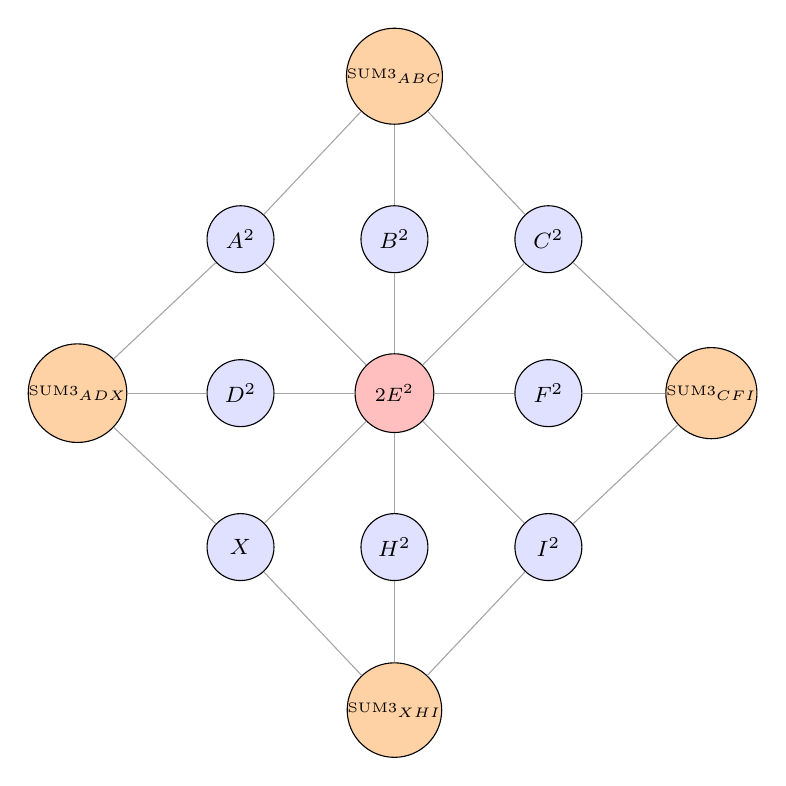
\begin{tikzpicture}[
  scale=1.15,
  cell/.style={circle, draw, fill=blue!12, minimum size=8.5mm,
               inner sep=0pt, font=\footnotesize},
  hub/.style={circle, draw, fill=red!25, minimum size=10mm,
              inner sep=0pt, font=\scriptsize},
  sum/.style={circle, draw, fill=orange!35, minimum size=11mm,
              inner sep=0pt, font=\tiny},
  lk/.style={draw, gray!70}
]
  \node[hub] (S2) at (0,0) {$2E^2$};
  \node[cell] (A) at (-1.7, 1.7) {$A^2$};
  \node[cell] (B) at ( 0  , 1.7) {$B^2$};
  \node[cell] (C) at ( 1.7, 1.7) {$C^2$};
  \node[cell] (D) at (-1.7, 0  ) {$D^2$};
  \node[cell] (F) at ( 1.7, 0  ) {$F^2$};
  \node[cell] (G) at (-1.7,-1.7) {$X$};
  \node[cell] (H) at ( 0  ,-1.7) {$H^2$};
  \node[cell] (I) at ( 1.7,-1.7) {$I^2$};
  \node[sum] (SABC) at ( 0  , 3.5) {SUM3$_{ABC}$};
  \node[sum] (SADG) at (-3.5, 0  ) {SUM3$_{ADX}$};
  \node[sum] (SCFI) at ( 3.5, 0  ) {SUM3$_{CFI}$};
  \node[sum] (SGHI) at ( 0  ,-3.5) {SUM3$_{XHI}$};
  \foreach \n in {A,B,C,D,F,G,H,I} \draw[lk] (\n) -- (S2);
  \foreach \n in {A,B,C} \draw[lk] (\n) -- (SABC);
  \foreach \n in {A,D,G} \draw[lk] (\n) -- (SADG);
  \foreach \n in {C,F,I} \draw[lk] (\n) -- (SCFI);
  \foreach \n in {G,H,I} \draw[lk] (\n) -- (SGHI);
\end{tikzpicture}
\end{center}

Each opposite pair --- $(A^2, I^2)$, $(B^2, H^2)$, $(C^2, X)$,
$(D^2, F^2)$ --- lies diametrically across the hub and sums to $2E^2$.
Adjoining the centre $E^2$ to any such pair yields a line, so the four
outer nodes take the common value
\[
\mathrm{SUM3}_{ABC} = \mathrm{SUM3}_{ADX} = \mathrm{SUM3}_{CFI}
= \mathrm{SUM3}_{XHI} = 3E^2 .
\]
The graph therefore encodes the whole system: the four pair relations
generate it, and the agreement of the four outer nodes is automatic.

\section{Three-Dimensional Form}

Placing the eight cells and the hub $2E^2$ in a base plane at height
$0$, and lifting each line-sum to height $3E^2$, gives a pyramid whose
apex projects onto the centre.

\begin{center}
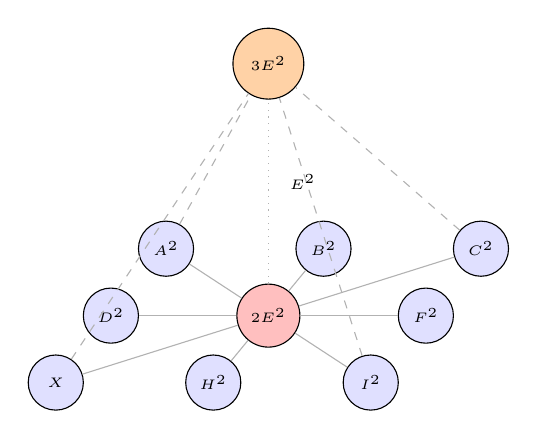
\begin{tikzpicture}[
  scale=1.0,
  cell/.style={circle, draw, fill=blue!12, minimum size=7mm,
               inner sep=0pt, font=\tiny},
  hub/.style={circle, draw, fill=red!25, minimum size=8mm,
              inner sep=0pt, font=\tiny},
  apex/.style={circle, draw, fill=orange!35, minimum size=9mm,
               inner sep=0pt, font=\tiny},
  lk/.style={draw, gray!60}
]
  \def\dx{0.55} \def\dy{0.30}
  \coordinate (o) at (0,0);
%  \node[cell] (A) at (-2*\dx+2*\dy, -2*\dy-2*\dx*0.0) {};
  % base square, drawn in oblique projection
  \foreach \i/\j/\lbl/\nm in {
    -1/1/A^2/A, 0/1/B^2/B, 1/1/C^2/C,
    -1/0/D^2/D, 1/0/F^2/F,
    -1/-1/X/G, 0/-1/H^2/H, 1/-1/I^2/I}
    {\node[cell] (\nm) at ({2.0*\i + 0.7*\j}, {0.85*\j}) {$\lbl$};}
  \node[hub] (S2) at (0,0) {$2E^2$};
  \foreach \n in {A,B,C,D,F,G,H,I} \draw[lk] (\n) -- (S2);
  \node[apex] (P) at (0,3.2) {$3E^2$};
  \foreach \n in {A,C,G,I} \draw[lk, dashed] (\n) -- (P);
  \draw[gray!60, dotted] (S2) -- (P);
  \node[font=\tiny, right] at (0.15,1.7) {$E^2$};
\end{tikzpicture}
\end{center}

Every line of the square consists of the centre together with one
opposite pair, so each of the four ascending edges rises from a pair
summing to $2E^2$ through the centre $E^2$ to the common apex $3E^2$.
The apex projects vertically onto $E^2$, and the height of the pyramid
is the magic sum.

\section{The Cone $u^2 + v^2 = 2e^2$}\label{sec:cone}

Write the entries of a nine-square magic square as $a^2, b^2, \dots, i^2$
with $X = g^2$. By Corollary~\ref{cor:pairs} the four opposite pairs
satisfy
\[
a^2 + i^2 = b^2 + h^2 = c^2 + g^2 = d^2 + f^2 = 2e^2 .
\]
Each is an instance of the single equation
\[
u^2 + v^2 = 2e^2 ,
\]
which in $(u,v,e)$-space is a homogeneous quadratic, hence a circular
cone with vertex at the origin and axis the line $u = v = e$. The plane
$e = \text{const}$ meets it in the circle $u^2 + v^2 = 2e^2$ of radius
$e\sqrt2$, on which the point $(e,e)$ always lies. This point is the
degenerate solution $u = v = e$, corresponding to the constant square.

\begin{center}
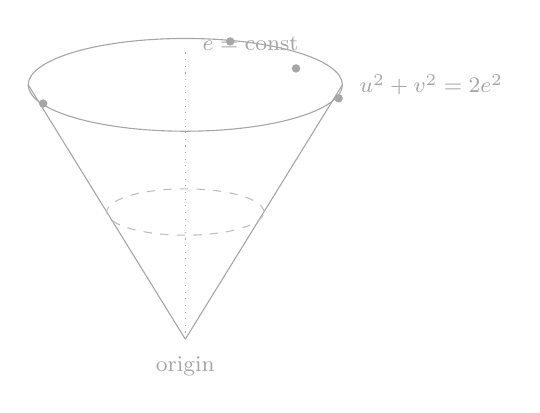
\begin{tikzpicture}[scale=0.95, gray!70]
  \draw (0,0) -- (-2.1,3.4); \draw (0,0) -- (2.1,3.4);
  \draw (0,3.4) ellipse (2.1 and 0.62);
  \draw[dotted] (0,0) -- (0,3.9);
  \draw[dashed, gray!50] (0,1.7) ellipse (1.05 and 0.31);
  \fill (1.48,3.62) circle (1.6pt);
  \fill (-1.9,3.15) circle (1.6pt);
  \fill (0.6,3.98) circle (1.6pt);
  \fill (2.05,3.22) circle (1.6pt);
  \node[font=\footnotesize, right] at (0.1,3.95) {$e = \text{const}$};
  \node[font=\footnotesize, right] at (2.2,3.4) {$u^2+v^2=2e^2$};
  \node[font=\footnotesize, below] at (0,-0.1) {origin};
\end{tikzpicture}
\end{center}

\begin{proposition}
A $3\times3$ magic square of nine perfect squares exists if and only if
there is an integer $e$ and four points
\[
(a,i),\ (b,h),\ (c,g),\ (d,f)
\]
with integer coordinates on the circle $u^2+v^2 = 2e^2$, pairwise
distinct as unordered pairs and none equal to $(e,e)$, satisfying the
single additional linear condition
\[
a^2 + b^2 + c^2 = 3e^2 .
\]
\end{proposition}

\begin{proof}
Corollary~\ref{cor:pairs} gives the four circle conditions, and the top
row gives the linear one; conversely, given such data, the
parametrisation of Section~\ref{sec:param} reconstructs the square, and
distinctness of the pairs is exactly distinctness of the entries.
\end{proof}

Thus the entire problem reduces to the arithmetic of one number.
Integer points on $u^2+v^2 = 2e^2$ correspond to representations of
$2e^2$ as a sum of two squares, whose number is governed by the primes
$p \equiv 1 \pmod 4$ dividing $e$; a candidate centre must therefore be
divisible by at least four such primes, or by prime powers supplying
the equivalent count. Every solution of $u^2+v^2=2e^2$ arises, up to
scaling, as
\[
u = m^2 + 2mn - n^2, \qquad
v = \lvert m^2 - 2mn - n^2 \rvert, \qquad
e = m^2 + n^2 ,
\]
so the four pairs are four choices of $(m,n)$ with common $e$.

\begin{remark}
The contrast with Theorem~\ref{thm:nolinear} is the point of this
section. The linear structure of the square is completely understood
and cannot obstruct a solution; the obstruction, if there is one, lies
in the impossibility of choosing four points on a single circle
$u^2+v^2=2e^2$ subject to one linear relation. This is a question about
representations by sums of two squares, and it is where the difficulty
of the problem resides. Intersecting the circle conditions with the
linear condition yields a curve of genus one, which is the route by
which elliptic curves enter the subject.
\end{remark}

\section{The Circle for $e = 425$}

Fix $e = 425$. The four opposite pairs of the square of
Section~\ref{sec:ex} give four points on the circle
\[
u^2 + v^2 = 2e^2 = 361250 ,
\]
of radius $425\sqrt2 \approx 601.04$. Two of these points have integer
coordinates and two do not:
\[
(205, 565), \quad (527, 289), \quad
\bigl(\sqrt{360721},\, 23\bigr), \quad
\bigl(373,\, \sqrt{222121}\bigr).
\]
The last two are the closing cells $B^2$ and $X$, whose entries are the
non-squares $360721$ and $222121$.

\begin{center}
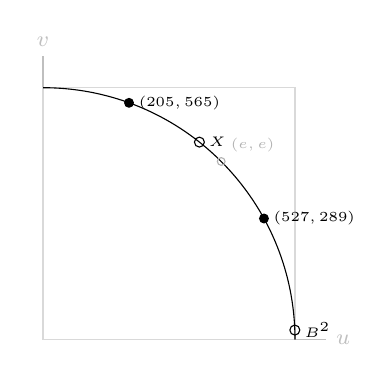
\begin{tikzpicture}[scale=1]
  \draw[gray!50] (0,0) -- (3.6,0) node[right, font=\footnotesize] {$u$};
  \draw[gray!50] (0,0) -- (0,3.6) node[above, font=\footnotesize] {$v$};
  \draw[gray!30] (0,0) rectangle (3.2,3.2);
  \draw (3.2,0) arc (0:90:3.2);
  \fill (1.092,3.008) circle (1.8pt)
    node[right, font=\tiny] {$(205,565)$};
  \fill (2.806,1.539) circle (1.8pt)
    node[right, font=\tiny] {$(527,289)$};
  \draw (3.198,0.122) circle (1.8pt)
    node[right, font=\tiny] {$B^2$};
  \draw (1.986,2.509) circle (1.8pt)
    node[right, font=\tiny] {$X$};
  \draw[gray!60] (2.263,2.263) circle (1.4pt)
    node[above right, font=\tiny] {$(e,e)$};
\end{tikzpicture}
\end{center}

All four points lie exactly on the circle: the pair identity
$u^2 + v^2 = 2e^2$ holds for every $3\times3$ magic square, whether or
not its entries are squares. What distinguishes the closing cells is
not their position but their coordinates --- filled points are integral,
open points are not.

\begin{remark}
The circle is inscribed in the square $[0, e\sqrt2]^2$, and it is
tempting to read the region between them as the failure of squareness.
This is not correct. Every magic square places its four pairs
\emph{on} the circle; the distinction is between integral and merely
real points of the same curve, and the integral points do not form a
region. A nine-square magic square requires all four points to be
lattice points, which is why the obstruction cannot be exhibited
geometrically and must be settled arithmetically.
\end{remark}

\section{Rotation and the Gaussian Integers}\label{sec:rotation}

The rotational picture of the previous section has an exact arithmetic
meaning. Identify the point $(u,v)$ on the circle $u^2+v^2 = 2e^2$ with
the Gaussian integer $u + vi$, whose norm is $2e^2$. Multiplication by
a Gaussian integer of norm $1$ --- that is, by $\pm1$ or $\pm i$ ---
permutes the point among the eight symmetries of the configuration,
while multiplication by a ratio $\pi/\bar\pi$, where $\pi$ is a prime
of norm $p \equiv 1 \pmod 4$ dividing $e$, rotates it to a
\emph{different} representation of the same norm.

\begin{center}
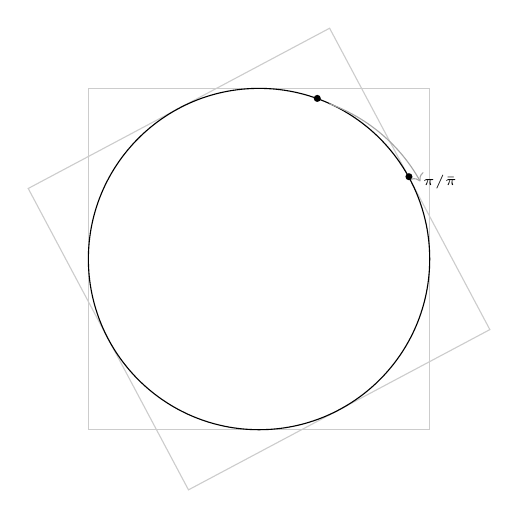
\begin{tikzpicture}[scale=0.85]
  \draw[gray!40] (-2.55,-2.55) rectangle (2.55,2.55);
  \draw[gray!40, rotate=28] (-2.55,-2.55) rectangle (2.55,2.55);
  \draw (0,0) circle (2.55);
  \fill (0.87,2.40) circle (1.5pt);
  \fill (2.24,1.23) circle (1.5pt);
  \draw[->, gray!70] (1.05,2.32) arc (70:29:2.55);
  \node[font=\tiny, right] at (2.3,1.15) {$\pi/\bar\pi$};
\end{tikzpicture}
\end{center}

\begin{center}
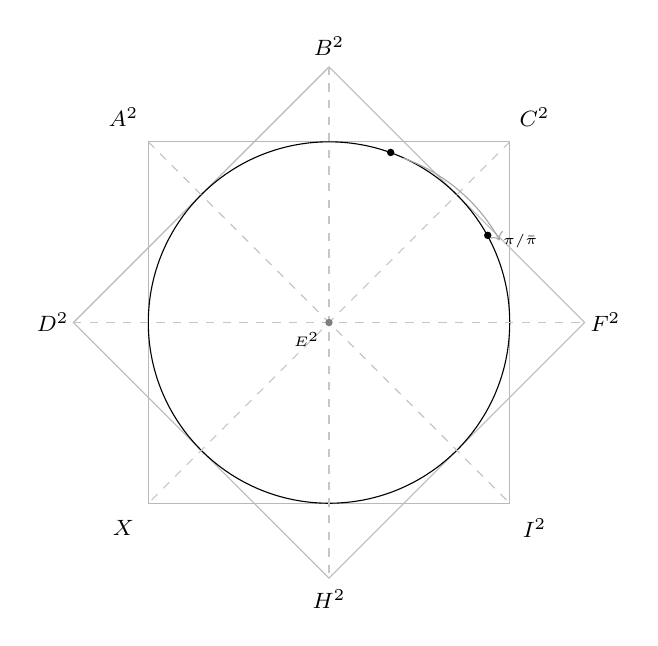
\begin{tikzpicture}[scale=0.9, font=\footnotesize]
  \draw[gray!55] (-2.55,-2.55) rectangle (2.55,2.55);
  \draw[gray!55, rotate=45] (-2.55,-2.55) rectangle (2.55,2.55);
  \draw (0,0) circle (2.55);
  \node at (-2.9, 2.9) {$A^2$};
  \node at ( 2.9, 2.9) {$C^2$};
  \node at (-2.9,-2.9) {$X$};
  \node at ( 2.9,-2.9) {$I^2$};
  \node at ( 0   , 3.9) {$B^2$};
  \node at ( 0   ,-3.9) {$H^2$};
  \node at (-3.9, 0   ) {$D^2$};
  \node at ( 3.9, 0   ) {$F^2$};
  \draw[gray!45, dashed] (-2.55,2.55) -- (2.55,-2.55);
  \draw[gray!45, dashed] (2.55,2.55) -- (-2.55,-2.55);
  \draw[gray!45, dashed] (0,3.61) -- (0,-3.61);
  \draw[gray!45, dashed] (-3.61,0) -- (3.61,0);
  \fill (0.87,2.40) circle (1.5pt);
  \fill (2.24,1.23) circle (1.5pt);
  \draw[->, gray!70] (1.05,2.32) arc (70:29:2.55);
  \node[font=\tiny, right] at (2.32,1.15) {$\pi/\bar\pi$};
  \fill[gray] (0,0) circle (1.5pt);
  \node[font=\tiny, below left] at (0,0) {$E^2$};
\end{tikzpicture}
\end{center}

\begin{center}
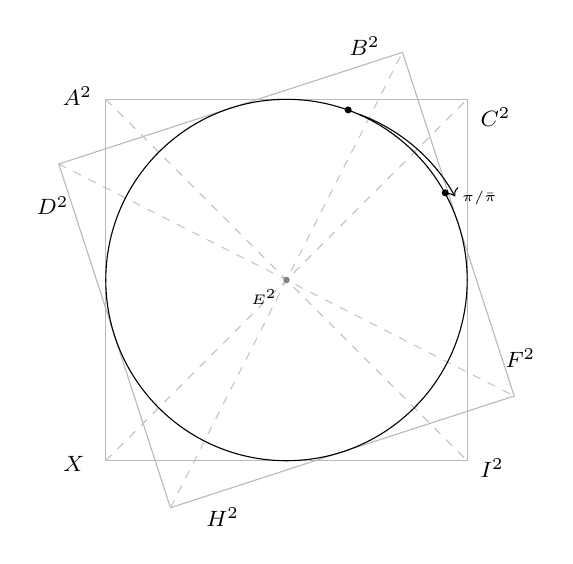
\begin{tikzpicture}[scale=0.9, font=\footnotesize]
  \draw[gray!55] (-2.55,-2.55) rectangle (2.55,2.55);
  \draw[gray!55, rotate=18] (-2.55,-2.55) rectangle (2.55,2.55);
  \draw[gray!45, dashed] (-2.55,-2.55) -- (2.55,2.55);
  \draw[gray!45, dashed] (-2.55, 2.55) -- (2.55,-2.55);
  \draw[gray!45, dashed, rotate=18] (-2.55,-2.55) -- (2.55,2.55);
  \draw[gray!45, dashed, rotate=18] (-2.55, 2.55) -- (2.55,-2.55);
  \draw (0,0) circle (2.55);
  \node at (-2.95, 2.60) {$A^2$};
  \node at ( 2.95, 2.30) {$C^2$};
  \node at (-3.00,-2.60) {$X$};
  \node at ( 2.90,-2.65) {$I^2$};
  \node at ( 1.10, 3.30) {$B^2$};
  \node at (-0.90,-3.35) {$H^2$};
  \node at (-3.30, 1.05) {$D^2$};
  \node at ( 3.30,-1.10) {$F^2$};
  \node[font=\tiny, below left] at (0,0) {$E^2$};
  \fill (0.87,2.40) circle (1.4pt);
  \fill (2.24,1.23) circle (1.4pt);
  \draw[->] (1.02,2.34) arc (70:29:2.55);
  \node[font=\tiny, right] at (2.34,1.15) {$\pi/\bar\pi$};
  \fill[gray] (0,0) circle (1.3pt);
\end{tikzpicture}
\end{center}

\begin{center}
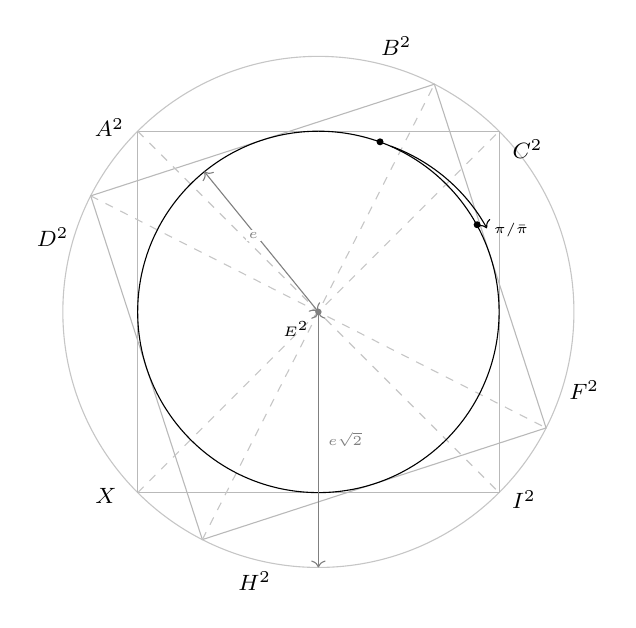
\begin{tikzpicture}[scale=0.9, font=\footnotesize]
  \draw[gray!45] (0,0) circle (3.606);
  \draw[gray!55] (-2.55,-2.55) rectangle (2.55,2.55);
  \draw[gray!55, rotate=18] (-2.55,-2.55) rectangle (2.55,2.55);
  \draw[gray!45, dashed] (-2.55,-2.55) -- (2.55,2.55);
  \draw[gray!45, dashed] (-2.55, 2.55) -- (2.55,-2.55);
  \draw[gray!45, dashed, rotate=18] (-2.55,-2.55) -- (2.55,2.55);
  \draw[gray!45, dashed, rotate=18] (-2.55, 2.55) -- (2.55,-2.55);
  \draw (0,0) circle (2.55);
  \draw[<->, gray] (0,0) -- (-1.61,1.98)
   node[midway, above left, font=\tiny, fill=white, inner sep=1pt] {$e$};
  \draw[<->, gray] (0,0) -- (0,-3.606)
    node[midway, right, font=\tiny] {$e\sqrt2$};
  \node at (-2.95, 2.60) {$A^2$};
  \node at ( 2.95, 2.30) {$C^2$};
  \node at (-3.00,-2.60) {$X$};
  \node at ( 2.90,-2.65) {$I^2$};
  \node at ( 1.10, 3.75) {$B^2$};
  \node at (-0.90,-3.80) {$H^2$};
  \node at (-3.75, 1.05) {$D^2$};
  \node at ( 3.75,-1.10) {$F^2$};
  \node[font=\tiny, below left] at (0,0) {$E^2$};
  \fill (0.87,2.40) circle (1.4pt);
  \fill (2.24,1.23) circle (1.4pt);
  \draw[->] (1.02,2.34) arc (70:29:2.55);
  \node[font=\tiny, right] at (2.34,1.15) {$\pi/\bar\pi$};
  \fill[gray] (0,0) circle (1.3pt);
\end{tikzpicture}
\end{center}


Thus the representations of $2e^2$ as a sum of two squares form a
single orbit under this rotation group, whose size is determined by the
factorisation of $e$: if
$e = 2^{\alpha} \prod p_j^{\,\beta_j} \prod q_k^{\,\gamma_k}$ with
$p_j \equiv 1$ and $q_k \equiv 3 \pmod 4$, the number of essentially
distinct representations grows with $\prod (2\beta_j + 1)$. A
nine-square magic square requires at least four of them, and hence a
centre divisible by several primes $p \equiv 1 \pmod 4$.

The three-dimensional form of the same statement is a rotation of the
pyramid of Section~8 about its axis: the base circle is carried to
itself, the apex is fixed, and the four ascending edges are permuted
among the available representations. The configuration is therefore
invariant under the rotation, and no rotation can separate the circle
from its circumscribed square.

\begin{remark}
This closes the geometric account. The rotation group acts transitively
on the representations, but which representations exist is a property
of the integer $e$ and not of the figure. Consequently neither the
planar nor the three-dimensional picture can decide the problem: they
exhibit the orbit, while the question is whether the orbit is large
enough, and suitably positioned, to satisfy the linear condition
$a^2+b^2+c^2 = 3e^2$. That question is arithmetic.
\end{remark}
\section{Two Kinds of Rotation}

The rotating-square figure admits two distinct motions, which should
not be conflated.

\subsection*{Symmetries of the square}

Rotation through a multiple of $90^\circ$, together with the four
reflections, generates the dihedral group $D_4$ of order $8$. In the
Gaussian picture these are multiplication by the units
$\pm 1, \pm i$ and conjugation, sending
\[
(u,v) \longmapsto (-v,u), \quad (-u,-v), \quad (v,-u), \quad (v,u),
\]
each of which preserves $u^2+v^2$. Applied to a magic square, such a
motion permutes the cells --- carrying $B^2$ to the position formerly
held by $F^2$, and so on --- while leaving the multiset of nine entries
unchanged. The result is the same square in a different orientation,
not a new solution. Every magic square therefore occurs in an orbit of
eight, and solutions are counted up to this action.

\subsection*{Rotation between representations}

The second motion is arithmetic. If $\pi$ is a Gaussian prime of norm
$p \equiv 1 \pmod 4$ dividing $e$, then multiplication by
$\pi / \bar\pi$, an element of norm $1$ but not a unit, carries a
lattice point of $u^2+v^2 = 2e^2$ to a \emph{different} lattice point
of the same circle. The angle of rotation is $2\arg\pi$, which is not
in general a multiple of $90^\circ$ and depends on $p$. For
$e = 425 = 5^2 \cdot 17$, this action carries $(205,565)$ to
$(527,289)$, exhibiting two of the four representations used by the
square of Section~\ref{sec:ex}.

\begin{remark}
The distinction is essential. Rotations of the first kind are available
for every $e$ and produce nothing new; rotations of the second kind
produce genuinely distinct representations, but only in numbers
governed by the factorisation of $e$. A nine-square magic square
requires four representations related by rotations of the second kind,
subject to $a^2+b^2+c^2 = 3e^2$. The figure displays the orbit; whether
a suitable quadruple exists within it is not a geometric question.
\end{remark}
\begin{center}
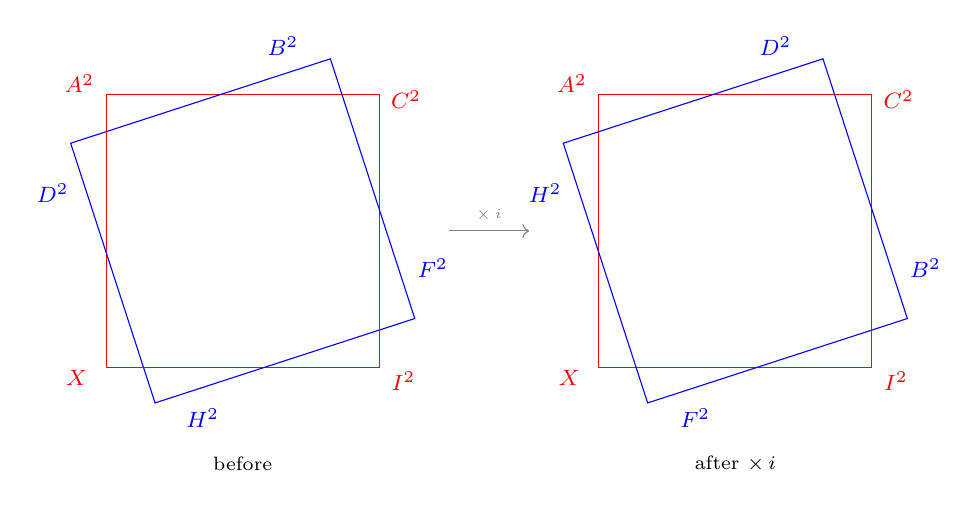
\begin{tikzpicture}[scale=0.68, font=\footnotesize]
  % --- left panel: before ---
  \begin{scope}[shift={(-4.6,0)}]
    \draw[red] (-2.55,-2.55) rectangle (2.55,2.55);
    \draw[blue, rotate=18] (-2.55,-2.55) rectangle (2.55,2.55);
    \node[red] at (-3.05, 2.75) {$A^2$};
    \node[red] at ( 3.05, 2.45) {$C^2$};
    \node[red] at (-3.10,-2.75) {$X$};
    \node[red] at ( 3.00,-2.80) {$I^2$};
    \node[blue] at ( 0.75, 3.45) {$B^2$};
    \node[blue] at (-0.75,-3.50) {$H^2$};
    \node[blue] at (-3.55, 0.70) {$D^2$};
    \node[blue] at ( 3.55,-0.70) {$F^2$};
    \node[font=\scriptsize] at (0,-4.35) {before};
  \end{scope}
  % --- arrow ---
  \draw[->, gray] (-0.75,0) -- (0.75,0)
    node[midway, above, font=\tiny] {$\times\, i$};
  % --- right panel: after a quarter turn ---
  \begin{scope}[shift={(4.6,0)}]
    \draw[red] (-2.55,-2.55) rectangle (2.55,2.55);
    \draw[blue, rotate=108] (-2.55,-2.55) rectangle (2.55,2.55);
    \node[red] at (-3.05, 2.75) {$A^2$};
    \node[red] at ( 3.05, 2.45) {$C^2$};
    \node[red] at (-3.10,-2.75) {$X$};
    \node[red] at ( 3.00,-2.80) {$I^2$};
    \node[blue] at ( 0.75, 3.45) {$D^2$};
    \node[blue] at (-0.75,-3.50) {$F^2$};
    \node[blue] at (-3.55, 0.70) {$H^2$};
    \node[blue] at ( 3.55,-0.70) {$B^2$};
    \node[font=\scriptsize] at (0,-4.35) {after $\times\, i$};
  \end{scope}
\end{tikzpicture}
\end{center}

\section{Search Design and the Closing Cells}

The reduction of Section~\ref{sec:cone} suggests an obvious search:
fix $e$, enumerate the integer points of $u^2+v^2 = 2e^2$, and select
two of them as the pairs $(a,i)$ and $(c,g)$, so that $A^2$, $I^2$,
$C^2$, $X$ and $E^2$ are square by construction. The remaining cells
$B^2$, $H^2$, $D^2$, $F^2$ are then determined, and one tests how many
of them are squares.

Each design answers a different question, and it is worth recording
which. Drawing $c$ from the list of representations forces
\[
X = 2e^2 - C^2
\]
to be a perfect square, so the search ranges over configurations in
which both pairs $(A^2, I^2)$ and $(C^2, X)$ are square. This is the
appropriate range for the nine-square question, where every cell must
be square in any case. It is a narrower range than the study of
intermediate configurations requires: in the square of
Section~\ref{sec:ex}, $X = 222121$ lies strictly between $471^2$ and
$472^2$, its non-square entries being precisely the closing cells
$B^2$ and $X$, so that configuration falls outside this range. At
$e = 425$ the constrained search accordingly returns only
configurations with the five square entries it guarantees by
construction.

Relaxing the constraint does not enlarge the supply of squares; it
admits configurations in which the non-square entries fall on the
closing cells. In both designs $C^2$ ranges over squares. What differs
is whether its partner $X = 2e^2 - C^2$ is required to be square as
well. Draw $a$ from the representations of $2e^2$, fixing the pair
$(A^2, I^2)$; then let $C^2$ range over all squares less than $2e^2$,
with $X$ free to be a non-square. The five remaining cells follow from
\eqref{eq:C}--\eqref{eq:F}, and the number of square entries is
counted rather than imposed.

\section{A Density Heuristic for the Closing Cells}

Suppose the pair $(C^2, X)$ is broken, so that $X$ is not a square.
Since
\[
B^2 - X = E^2 - A^2 ,
\]
the value of $B^2$ differs from $X$ by a fixed amount, and is
therefore also a non-square except by coincidence. The count of square
entries then turns on the single remaining cell
\[
H^2 = 2E^2 - B^2 = E^2 + A^2 - X ,
\]
which is square in a seven-square configuration and not in a
six-square one.

The magnitude of $H^2$ is governed by $A$ relative to $E$. Writing
$A = \alpha E$ with $\alpha > 0$, we have
$H^2 = (1 + \alpha^2)E^2 - X$, so $H^2$ is small when $\alpha < 1$ and
large when $\alpha > 1$, for $X$ in the admissible range. Since
consecutive squares near $n$ differ by approximately $2\sqrt n$, the
proportion of integers near $n$ that are squares decreases like
$n^{-1/2}$. A small forced value of $H^2$ therefore has a higher
chance of being square than a large one.

This gives a heuristic account of the two configurations at
$e = 425$. With $A = 205 < E$, the forced value is $H^2 = 529 = 23^2$,
and the square attains seven square entries. With $A = 527 > E$, the
same construction forces $H^2 = 236233$, which lies between $486^2$
and $487^2$, and the count falls to six. The known seven-square
example accordingly has $A < E$.

\begin{remark}
The argument is heuristic and not a proof. It gives a reason to expect
seven-square configurations to be found more readily when $A < E$, but
it excludes nothing: $H^2$ is a specific integer, not a random one, and
large squares occur freely elsewhere in the same square --- for
instance $F^2 = 565^2 = 319225$. Establishing that no seven-square
configuration exists with $A > E$ at a given $e$ would require an
exhaustive check over the admissible values of $C$, which the density
argument does not supply.
\end{remark}

\section{Admissibility and the Choice of $A$}

Fix $E$ and $C$, so that $X = 2E^2 - C^2$ is determined, and write
\[
\delta_{\text{real}} = X - E^2 .
\]
The parametrisation then gives
\[
H^2 = A^2 - \delta_{\text{real}}, \qquad F^2 = A^2 + \delta_{\text{real}} ,
\]
so $H^2$ is positive precisely when $A > \sqrt{\delta_{\text{real}}}$. This is a
genuine restriction: roots below the threshold cannot serve as $A$ at
all, independently of any squareness condition.

Among the admissible roots, $H^2 = A^2 - \delta_{\text{real}}$ is increasing in $A$.
The smallest admissible root therefore yields the smallest forced value
of $H^2$. Since consecutive squares near $n$ differ by roughly
$2\sqrt n$, the density of squares near $n$ falls like $n^{-1/2}$, and a
smaller forced value has a correspondingly better chance of being
square. This gives a heuristic rule:

\begin{quote}
Among the roots available at a given centre, the most promising choice
of $A$ is the smallest one exceeding $\sqrt{\delta_{\text{real}}}$.
\end{quote}

At $E = 425$ with $C = 373$ we have $X = 222121$ and
$\delta_{\text{real}} = 41496$, so $\sqrt{\delta_{\text{real}}} \approx 203.7$. The available roots
are $23, 205, 289, 373, 527, 565$; the root $23$ falls below the
threshold and is inadmissible, and $205$ is the smallest root above it.
It yields $H^2 = 529 = 23^2$, and the resulting square attains seven
square entries. The next admissible root, $289$, yields
$H^2 = 42025 = 205^2$ --- still square, but the configuration achieves
only six, the $D/F$ pair failing instead.

\begin{remark}
Two cautions. First, the rule is heuristic: $H^2$ is a determinate
integer, and its squareness is not a matter of probability. The example
above shows the rule identifying the best configuration while the
decisive failure at $A = 289$ occurs elsewhere in the square, at the
pair $(D^2, F^2)$. Second, replacing $A$ by its partner
$\sqrt{2E^2 - A^2}$ is the reflection across the anti-diagonal, which
permutes the entries without altering their multiset; the count is
therefore invariant under that exchange, and one may normalise to
$A < E$ without loss.
\end{remark}

\section{An Admissibility Threshold}

\begin{proposition}\label{prop:threshold}
Fix $E$ and $C$, and set $X = 2E^2 - C^2$ and $\delta_{\text{real}} = X - E^2$. Then
\[
H^2 = A^2 - \delta_{\text{real}}, \qquad F^2 = A^2 + \delta_{\text{real}} ,
\]
and the nine entries are all positive only if
\[
A > \sqrt{\delta_{\text{real}}} \quad\text{when } \delta_{\text{real}} > 0,
\qquad
A > \sqrt{-\delta_{\text{real}}} \cdot 0 \ \ \text{(no lower constraint)}
\quad\text{when } \delta_{\text{real}} \le 0 .
\]
\end{proposition}

\begin{proof}
From \eqref{eq:H}, $H^2 = E^2 + A^2 - X = A^2 - \delta_{\text{real}}$, and from
\eqref{eq:F}, $F^2 = A^2 + X - E^2 = A^2 + \delta_{\text{real}}$. If $\delta_{\text{real}} > 0$
then $H^2 > 0$ requires $A^2 > \delta_{\text{real}}$; if $\delta_{\text{real}} \le 0$ then
$H^2 \ge A^2 > 0$ automatically, while $F^2 > 0$ requires
$A^2 > -\delta_{\text{real}}$. In either case the smaller of the two cells imposes
the bound $A^2 > |\delta_{\text{real}}|$.
\end{proof}

\begin{corollary}
Roots $A$ with $A^2 \le |\delta_{\text{real}}|$ are inadmissible: no magic square
with positive entries has that value in the corner cell, whatever the
squareness of the remaining cells.
\end{corollary}

The threshold is a strict consequence of the parametrisation, not a
heuristic. It applies before any question of squareness arises, and it
removes candidates from the search unconditionally.

At $E = 425$ with $C = 373$ one has $X = 222121$ and
$\delta_{\text{real}} = 41496$, whence $\sqrt{\delta_{\text{real}}} \approx 203.7$. Of the roots
$23, 205, 289, 373, 527, 565$ occurring at this centre, the root $23$
lies below the threshold and is inadmissible; the remaining five are
admissible. Taking $A = 205$, the smallest admissible root, gives
$H^2 = 42025 - 41496 = 529 = 23^2$, and the configuration attains seven
square entries.

\begin{remark}
Since $H^2 = A^2 - \delta_{\text{real}}$ increases with $A$, the smallest admissible
root produces the smallest forced value of $H^2$. As the density of
squares near $n$ decreases like $n^{-1/2}$, this suggests examining the
smallest admissible root first. That suggestion is heuristic;
Proposition~\ref{prop:threshold} itself is not.
\end{remark}

\section{An Admissibility Threshold}

\begin{proposition}\label{prop:threshold}
Fix $E$ and $C$, and set $X = 2E^2 - C^2$ and $\delta_{\text{real}} = X - E^2$. Then
\[
H^2 = A^2 - \delta_{\text{real}}, \qquad F^2 = A^2 + \delta_{\text{real}} ,
\]
and all nine entries are positive if and only if
\[
A^2 > \lvert \delta_{\text{real}} \rvert = \lvert X - E^2 \rvert .
\]
\end{proposition}

\begin{proof}
From \eqref{eq:H}, $H^2 = E^2 + A^2 - X = A^2 - \delta_{\text{real}}$; from
\eqref{eq:F}, $F^2 = A^2 + X - E^2 = A^2 + \delta_{\text{real}}$. Their minimum is
$A^2 - \lvert\delta_{\text{real}}\rvert$, so both are positive exactly when
$A^2 > \lvert\delta_{\text{real}}\rvert$. Equality gives a vanishing entry, which is
excluded. The remaining cells are positive whenever $C^2 < 2E^2$ and
$A^2 < 2E^2$, which the choice of $C$ and $A$ already assumes.
\end{proof}

\begin{corollary}
Any $A$ with $A^2 \le \lvert X - E^2\rvert$ is inadmissible: no magic
square with positive entries carries that value in the corner cell.
\end{corollary}

The bound is a consequence of the parametrisation alone. Its
derivation uses only the linear identities
\eqref{eq:H} and \eqref{eq:F}, and makes no assumption about whether
$X$, $A^2$, or any other entry is a perfect square. It therefore
applies to every configuration --- including those, such as the square
of Section~\ref{sec:ex}, in which $X$ is not a square --- and may be
used to prune a search before any squareness test is performed.

At $E = 425$ with $C = 373$ one has $X = 222121$, which is not a
square, and $\delta_{\text{real}} = 41496$, so $\lvert\delta_{\text{real}}\rvert^{1/2} \approx
203.7$. Of the roots $23, 205, 289, 373, 527, 565$ occurring at this
centre, only $23$ falls below the threshold. Taking $A = 205$, the
smallest admissible root, gives $H^2 = 42025 - 41496 = 529 = 23^2$ and
a configuration with seven square entries.

\begin{remark}
Since $H^2 = A^2 - \delta_{\text{real}}$ increases with $A$ when $\delta_{\text{real}} > 0$, the
smallest admissible root produces the smallest forced value of $H^2$;
as the density of squares near $n$ decreases like $n^{-1/2}$, this
suggests testing that root first. The suggestion is heuristic.
Proposition~\ref{prop:threshold} is not.
\end{remark}

\section{The Two Conditions, Side by Side}

The two conditions defining the problem are of different kinds and live
in different coordinate planes. The left panel shows the pair condition
$u^2+v^2=2e^2$, satisfied by every magic square; the right panel shows
the squareness condition $y = x^2$, on which only some of the entries
lie.

\begin{center}
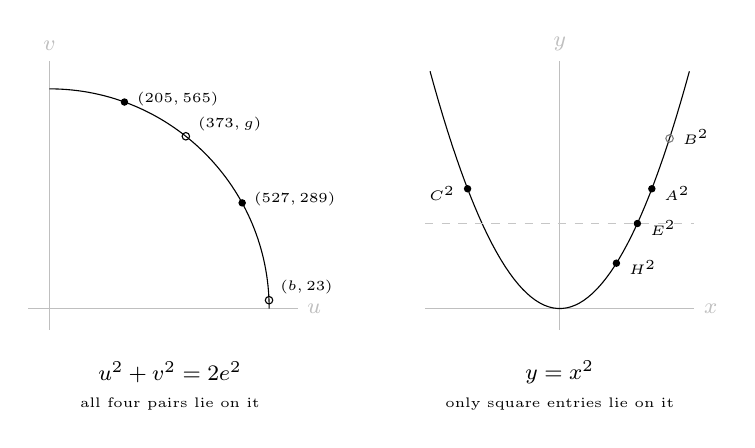
\begin{tikzpicture}[scale=0.9, font=\footnotesize]
  % --- left: the circle ---
  \begin{scope}
    \draw[gray!50] (-0.3,0) -- (3.5,0) node[right] {$u$};
    \draw[gray!50] (0,-0.3) -- (0,3.5) node[above] {$v$};
    \draw (3.1,0) arc (0:90:3.1);
    \fill (1.058,2.914) circle (1.5pt);
    \fill (2.719,1.491) circle (1.5pt);
    \draw (3.098,0.118) circle (1.5pt);
    \draw (1.924,2.431) circle (1.5pt);
    \node[font=\tiny, right] at (1.1,2.95) {$(205,565)$};
    \node[font=\tiny, right] at (2.75,1.55) {$(527,289)$};
    \node[font=\tiny, right] at (3.12,0.30) {$(b,23)$};
    \node[font=\tiny, right] at (1.96,2.60) {$(373,g)$};
    \node at (1.7,-0.9) {$u^2+v^2=2e^2$};
    \node[font=\tiny] at (1.7,-1.35) {all four pairs lie on it};
  \end{scope}
  % --- right: the parabola ---
  \begin{scope}[shift={(7.2,0)}]
    \draw[gray!50] (-1.9,0) -- (1.9,0) node[right] {$x$};
    \draw[gray!50] (0,-0.3) -- (0,3.5) node[above] {$y$};
    \draw[domain=-1.83:1.83, samples=60] plot (\x, {\x*\x});
    \fill (1.30,1.69) circle (1.5pt);
    \fill (-1.30,1.69) circle (1.5pt);
    \fill (0.80,0.64) circle (1.5pt);
    \draw[gray] (1.55,2.40) circle (1.5pt);
    \node[font=\tiny, right] at (1.34,1.62) {$A^2$};
    \node[font=\tiny, left]  at (-1.34,1.62) {$C^2$};
    \node[font=\tiny, right] at (0.84,0.58) {$H^2$};
    \node[font=\tiny, right] at (1.60,2.42) {$B^2$};
    \node at (0,-0.9) {$y = x^2$};
    \node[font=\tiny] at (0,-1.35) {only square entries lie on it};
    \draw[gray!45, dashed] (-1.9,1.20) -- (1.9,1.20);
    \fill (1.096,1.20) circle (1.5pt);
    \node[font=\tiny, right] at (1.14,1.14) {$E^2$};
  \end{scope}
\end{tikzpicture}
\end{center}

In the left panel all four pairs of any magic square lie exactly on the
circle, since $u^2+v^2 = 2e^2$ is an identity of the family; two of the
four have integer coordinates and two, marked hollow, do not. In the
right panel an entry $n$ appears as the point $(\sqrt n, n)$, which is a
lattice point precisely when $n$ is a perfect square; the entry $B^2$,
marked hollow, is not.

\begin{remark}
The two panels cannot be superimposed. The axes of the left are two
roots $u, v$; the axes of the right are a root and its square. A
scaling of the circle therefore cannot carry it onto the parabola, and
no single figure displays both conditions at once. This separation is
the geometric counterpart of Theorem~\ref{thm:nolinear}: the pair
condition is uniform across the family and visible, while the
squareness condition is arithmetic and is not.
\end{remark}

\section{The Pairs as Bisected Segments}

Plotting each entry at its own value and drawing the horizontal line
$y = E^2$ gives the magic condition in its simplest form: every
opposite pair is a vertical segment bisected by that line.

\begin{center}
\begin{tikzpicture}[y=0.000016cm, x=1cm, font=\footnotesize]
  \draw[thick] (-0.4,180625) -- (8.4,180625);
  \node[left] at (-0.5,180625) {$E^2$};
  % A / I
  \draw[blue!70] (1,42025) -- (1,319225);
  \fill (1,42025) circle (2pt);  \node[below] at (1,42025) {$A^2$};
  \fill (1,319225) circle (2pt); \node[above] at (1,319225) {$I^2$};
  % B / H
  \draw[blue!70] (3,529) -- (3,360721);
  \fill (3,529) circle (2pt);    \node[below] at (3,529) {$H^2$};
  \fill (3,360721) circle (2pt); \node[above] at (3,360721) {$B^2$};
  % C / X
  \draw[blue!70] (5,139129) -- (5,222121);
  \fill (5,139129) circle (2pt); \node[below] at (5,139129) {$C^2$};
  \fill (5,222121) circle (2pt); \node[above] at (5,222121) {$X$};
  % D / F
  \draw[blue!70] (7,83521) -- (7,277729);
  \fill (7,83521) circle (2pt);  \node[below] at (7,83521) {$F^2$};
  \fill (7,277729) circle (2pt); \node[above] at (7,277729) {$D^2$};
  % midpoint marks
  \foreach \x in {1,3,5,7} \fill[red!70] (\x,180625) circle (1.6pt);
\end{tikzpicture}
\end{center}

The four segments are drawn to scale for the square of
Section~\ref{sec:ex}. Each is bisected by $y = E^2$, since
$A^2 + I^2 = B^2 + H^2 = C^2 + X = D^2 + F^2 = 2E^2$; the marked
midpoints all coincide in height with the line. The segments differ
greatly in length --- from $82992$ for the pair $(C^2, X)$ to $360192$
for $(B^2, H^2)$ --- and their lengths are the only freedom the magic
condition leaves, the three independent half-lengths being the three
parameters of the family.

\begin{remark}
The figure displays the magic condition completely and says nothing
about squareness: it is identical in form for every $3\times3$ magic
square. The entries $B^2 = 360721$ and $X = 222121$ are not squares,
yet their segments are bisected exactly as the others are.
\end{remark}


\section{The Pairs as Segments of Equal Length}

Each opposite pair may be drawn as a vertical segment whose lower
endpoint is the smaller entry and whose upper endpoint is the larger,
both measured from a common baseline at $0$. Since
\[
A^2 + I^2 = B^2 + H^2 = C^2 + X = D^2 + F^2 = 2E^2 ,
\]
the difference between the endpoints is not constant, but the
\emph{sum} is; drawing each segment so that its length equals that sum
renders all four segments congruent, of common length $2E^2$. The four
pairs then differ only in elevation.

\begin{center}
\begin{tikzpicture}[y=3cm, x=1cm, font=\footnotesize]
  \draw[gray!50] (-0.4,0) -- (8.6,0) node[right] {$0$};
  \draw[gray!40, dashed] (-0.4,1) -- (8.6,1) node[right] {$2E^2$};
  \foreach \x/\lo/\hi/\ln/\hn in {
      1/0.1163/1.1163/A^2/I^2,
      3/0.0015/1.0015/H^2/B^2,
      5/0.3851/1.3851/C^2/X,
      7/0.2312/1.2312/F^2/D^2}
    {\draw[blue!70, line width=1.2pt] (\x,\lo) -- (\x,\hi);
     \fill[red!75] (\x,\lo) circle (2pt);
     \node[right, font=\tiny] at (\x,\lo) {$\ln$};
     \node[above, font=\tiny] at (\x,\hi) {$\hn$};}
  \draw[gray!40, dashed] (-0.4,0.5) -- (8.6,0.5) node[right] {$E^2$};
\end{tikzpicture}
\end{center}

The figure is drawn to scale for the square of
Section~\ref{sec:ex}, with heights expressed as fractions of $2E^2 =
361250$. The bases sit at
\[
\tfrac{H^2}{2E^2} = 0.0015, \quad
\tfrac{A^2}{2E^2} = 0.1163, \quad
\tfrac{F^2}{2E^2} = 0.2312, \quad
\tfrac{C^2}{2E^2} = 0.3851 ,
\]
and each summit follows at exactly one unit above.

Three features are worth noting. The congruence of the segments is the
magic condition itself, expressed without arithmetic: it is what
$u + v = 2E^2$ looks like when $u$ and $v$ are drawn as the ends of a
single interval. The elevation of each segment is unconstrained, and
the three independent elevations are precisely the three parameters of
the family, the fourth being determined once the others are chosen.
Finally, a segment based at height $E^2$ would have both endpoints
equal to $E^2$; the distance of each base below that level therefore
measures how far the corresponding pair is from the degenerate
configuration.

\begin{remark}
As with the preceding figures, the picture is indifferent to
squareness. The segments for $(C^2, X)$ and $(B^2, H^2)$ are congruent
to the others and equally well placed, although $X = 222121$ and
$B^2 = 360721$ are not perfect squares.
\end{remark}

\section{The Two Quadrilaterals}

Joining the four corner cells $A^2, I^2, X, C^2$ and, separately, the
four edge cells $H^2, B^2, D^2, F^2$, each set forms a parallelogram:
the two segments in each set are congruent, of length $2E^2$, so
opposite sides are parallel by construction.

\begin{center}
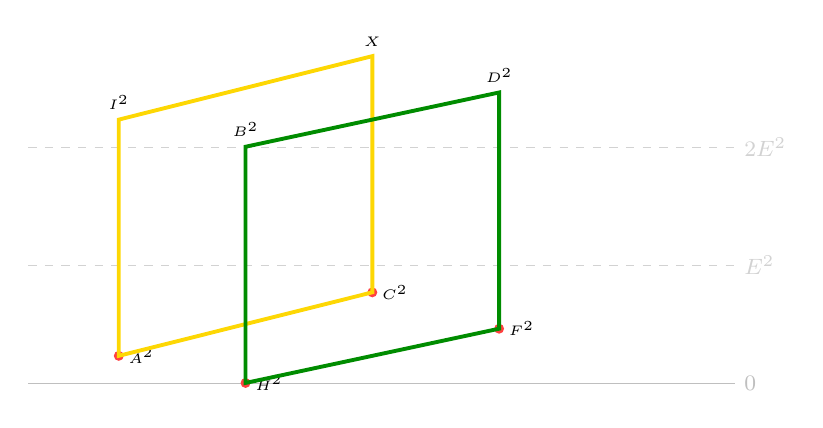
\begin{tikzpicture}[y=3cm, x=1.15cm, font=\footnotesize]
  \draw[gray!50] (-0.4,0) -- (7.4,0) node[right] {$0$};
  \draw[gray!35, dashed] (-0.4,0.5) -- (7.4,0.5) node[right] {$E^2$};
  \draw[gray!35, dashed] (-0.4,1) -- (7.4,1) node[right] {$2E^2$};
  % --- the four segments ---
  \foreach \x/\lo/\hi/\ln/\hn in {
      0.6/0.1163/1.1163/A^2/I^2,
      2.0/0.0015/1.0015/H^2/B^2,
      3.4/0.3851/1.3851/C^2/X,
      4.8/0.2312/1.2312/F^2/D^2}
    {\draw[blue!55, line width=1pt] (\x,\lo) -- (\x,\hi);
     \fill[red!75] (\x,\lo) circle (1.8pt);
     \node[right, font=\tiny] at (\x,\lo) {$\ln$};
     \node[above, font=\tiny] at (\x,\hi) {$\hn$};}
  % --- corner-cell parallelogram: A, I, X, C ---
  \draw[yellow!75!orange, line width=1.4pt]
    (0.6,0.1163) -- (0.6,1.1163) -- (3.4,1.3851)
    -- (3.4,0.3851) -- cycle;
  % --- edge-cell parallelogram: H, B, D, F ---
  \draw[green!55!black, line width=1.4pt]
    (2.0,0.0015) -- (2.0,1.0015) -- (4.8,1.2312)
    -- (4.8,0.2312) -- cycle;
\end{tikzpicture}
\end{center}

The yellow quadrilateral carries the corner cells and the green the
edge cells; they correspond respectively to the upright and the rotated
square of the figure in Section~\ref{sec:rotation}, in which the same
two sets appear as the vertices of two squares inscribed in the circle
$u^2 + v^2 = 2E^2$. Since each vertical side has length $2E^2$, both
quadrilaterals are parallelograms of equal side length, differing only
in the elevations of their two sides.

\begin{remark}
The correspondence between the two figures is exact: a pair of cells is
a vertical side here and a diameter there, and in both cases the
defining relation is $u + v = 2E^2$. Neither figure registers whether
an individual entry is a perfect square.
\end{remark}
\section{The Partner Function and Automatic Pair Generation}\label{sec:partner}

The identity $u^2+v^2=2E^2$ of Corollary~\ref{cor:pairs} may be turned
into a function that manufactures partners on demand, converting the
search of Section~\ref{sec:cone} into a short finite computation.

\begin{definition}\label{def:fg}
For $w \ge 0$ define
\[
f(w) = \Bigl(\sqrt w\,(\sqrt w + 1) - \sqrt w\Bigr)^{1/2},
\qquad
g(x) = f\bigl(2E^2 - x\bigr), \qquad x \le 2E^2 .
\]
\end{definition}

Although $f$ is written as a nested radical, it collapses algebraically:
\[
\sqrt w\,(\sqrt w+1)-\sqrt w = w+\sqrt w-\sqrt w = w ,
\]
so $f(w)=\sqrt w$ identically, and hence $g(x) = \sqrt{2E^2-x}$. The
nested form is kept here only because it is the one in which the
function was first written down; numerically the two forms agree, but
the nested form accumulates more floating-point error, performing three
chained square roots where one suffices.

\begin{proposition}\label{prop:partner}
For every $x \le 2E^2$, writing $v=g(x)$ gives $x+v^2=2E^2$
identically.
\end{proposition}

\begin{proof}
$v^2 = g(x)^2 = 2E^2-x$ by Definition~\ref{def:fg}.
\end{proof}

Proposition~\ref{prop:partner} is the mechanism, not a discovery: it
guarantees the pair relation for \emph{any} input $x$, whether or not
$v$ is itself an integer. To search for pairs of \emph{cells} --- both
members squares of integers --- apply $g$ to a squared root rather than
to a raw value:
\[
q(x) = g(x^2) = \sqrt{2E^2-x^2}, \qquad r(x) = q(x)^2 = 2E^2-x^2 .
\]
By Proposition~\ref{prop:partner}, $x^2+q(x)^2=2E^2$ holds for every
integer $x$; what varies is only whether $q(x)$ is itself an integer.

\begin{proposition}[Automatic pair generation]\label{prop:autogen}
For given $E$, the set
\[
\mathcal P(E) = \bigl\{\, (x,\,q(x)) : 1 \le x \le E,\ q(x) \in
\mathbb Z \,\bigr\}
\]
is exactly the set of representations of $2E^2$ as a sum of two
positive squares (Section~\ref{sec:rotation}), together with the
degenerate pair $(E,E)$. Every element of $\mathcal P(E)$ may be
assigned to any one of the three symmetric opposite-pair roles $(A,I)$,
$(D,F)$, $(H,B)$, since each satisfies the same identity
$u^2+v^2=2E^2$ underlying all three, and none of the three formulas
\eqref{eq:C}--\eqref{eq:F} distinguishes which role a given
representation fills.
\end{proposition}

This turns the search into a scan: for $x=1,\dots,\lfloor E\sqrt2
\rfloor$, retain those $x$ with $r(x)$ a perfect square, and read off
the pair $(x,q(x))$. At $E=425$ the scan returns exactly the seven
pairs
\[
(7,601),\ (85,595),\ (175,575),\ (205,565),\ (289,527),\
(329,503),\ (355,485),
\]
together with the degenerate $(425,425)$. Assigning
$(A,I)=(205,565)$ and $(F,D)=(289,527)$ --- two of the seven pairs,
chosen with no further arithmetic --- reproduces the square of
Section~\ref{sec:ex} completely once run through
\eqref{eq:C}--\eqref{eq:F}: $C=373$, $H=23$, $X=222121$, and
$B=360721$ follow immediately. Five of the nine cells, $E,A,I,F,D$, are
guaranteed square by this construction alone, before any further
search; the remaining question --- whether $C,X,H,B$ also cooperate ---
is exactly the content of the sections that follow.

\section{Closing the Third Pair in Closed Form}\label{sec:closedform}

Section~\ref{sec:partner} showed that drawing two of the three
symmetric pairs directly from $\mathcal P(E)$ --- say $(A,I)$ and
$(D,F)$ --- guarantees five squares for free. It is natural to ask
whether a \emph{third} pair, $(C,X)$, can be tested just as cheaply,
without scanning a probe $x$ against a lookup table. It can: the first
column of the square supplies a second identity that, combined with
Corollary~\ref{cor:pairs}, pins $C$ down in one step.

\begin{proposition}\label{prop:closedform}
For any positive integers $A,D$, set $X = 3E^2-A^2-D^2$, the value
forced by the first-column condition $A^2+D^2+X=3E^2$. Then
\[
C^2 = A^2+D^2-E^2
\]
identically, so $C$ is an integer precisely when $A^2+D^2-E^2$ is a
non-negative perfect square --- with no search over $X$, and no table
of the values $r(x)$, required.
\end{proposition}

\begin{proof}
By Corollary~\ref{cor:pairs}, $C^2+X=2E^2$, so $C^2=2E^2-X$.
Substituting $X=3E^2-A^2-D^2$ gives
$C^2 = 2E^2-(3E^2-A^2-D^2) = A^2+D^2-E^2$.
\end{proof}

The other closing cell, $B^2$, closes in the same way, from the top
row rather than the first column.

\begin{proposition}\label{prop:closedformB}
For any positive integers $A,D$, with $C^2=A^2+D^2-E^2$ as in
Proposition~\ref{prop:closedform},
\[
B^2 = 4E^2 - 2A^2 - D^2
\]
identically, the value forced by the top-row condition
$A^2+B^2+C^2=3E^2$.
\end{proposition}

\begin{proof}
$B^2 = 3E^2-A^2-C^2 = 3E^2-A^2-(A^2+D^2-E^2) = 4E^2-2A^2-D^2$.
\end{proof}

At $E=425$, $A=205$, $D=527$: $B^2=4(425)^2-2(205)^2-527^2=360721$,
matching the square of Section~\ref{sec:ex} exactly, with the same
no-search, single-\texttt{isqrt} character as Proposition~\ref{prop:closedform}.
Between them, Propositions~\ref{prop:closedform}
and~\ref{prop:closedformB} give both closing cells of
Section~\ref{sec:ex} --- $X$ and $B^2$ --- as explicit closed-form
functions of the seed $(A,D)$ and the centre $E$ alone, with no
intermediate cell and no search over either.

Proposition~\ref{prop:closedform} is the closed form of the check that
the table $\{r(x)\}$ was performing implicitly: testing whether the
column's forced $X$ equals $r(x)=2E^2-x^2$ for some $x$ is the same
test as asking whether $2E^2-X$ --- namely $A^2+D^2-E^2$ --- is itself
a perfect square, and the latter needs no table at all. What was an
$O(E)$ membership test against a precomputed set collapses to a single
\texttt{isqrt} check per candidate pair $(A,D)$.

At $E=425$, applying Proposition~\ref{prop:closedform} to every ordered
pair drawn from $\mathcal P(425)$ recovers $C^2=205^2+527^2-425^2=
139129=373^2$ at once --- the square of Section~\ref{sec:ex} --- with
no scan. The same closed form also flags two further admissible,
distinct-cell configurations, $(A,D)=(527,85)$ and $(527,205)$, each
reaching six squares ($E,A,I,D,F,C$) but not seven: swapping which
member of a pair is labelled $A$ rather than $D$ changes the forced
$H^2=E^2+A^2-X$, and in these two cases $H^2$ fails to be square where,
for $(A,D)=(205,527)$, it happens to succeed. This sharpens the moral
of Section~\ref{sec:parity}: reaching seven squares is not a property
of \emph{which} representations are used, but of the specific
role-assignment among them, and Proposition~\ref{prop:closedform} makes
that assignment cheap enough to check exhaustively.

\begin{remark}
Writing $S=A^2+D^2$, Proposition~\ref{prop:closedform} and the corner
identity $C^2+X=2E^2$ together read as two complementary measurements
of the same quantity:
\[
C^2 = S - E^2, \qquad X = 3E^2 - S .
\]
Adding them cancels $S$ entirely, $C^2+X = (S-E^2)+(3E^2-S) = 2E^2$,
recovering Corollary~\ref{cor:pairs} for this pair regardless of what
$S$ is. $C^2$ measures how far $A^2+D^2$ sits above the centre value
$E^2$; $X$ measures how far it falls short of the magic sum $3E^2$; and
the two measurements are complementary simply because $E^2$ and $3E^2$
are themselves symmetric about $2E^2$.
\end{remark}

\begin{remark}
This complementarity is purely algebraic and carries no arithmetic
force: it says nothing about whether $C$ and $\sqrt X$ are integers,
only that whichever real values they take, their squares sum correctly.
Squareness of $C$ (Proposition~\ref{prop:closedform}) and squareness of
$X$ are two independent conditions on the same derived quantity $C^2$
--- the first, that $S-E^2$ is a perfect square; the second, that $C$
is itself a member of $\mathcal P(E)$, i.e.\ that $2E^2-C^2$ is
\emph{also} a perfect square. Requiring both is a strictly rarer event
than requiring either alone: an exhaustive check over every ordered
triple drawn from $\mathcal P(E)$ finds no $(A,D,C)$, at either
$E=425$ or $E=1105$, with $C$ satisfying Proposition~\ref{prop:closedform}
\emph{and} lying in $\mathcal P(E)$ simultaneously. Beyond the
guaranteed five ($E,A,I,D,F$) and the sixth cell $C$ of
Proposition~\ref{prop:closedform}, every configuration found in
Sections~\ref{sec:closedform}--\ref{sec:parity} that reaches a seventh
square gets it from $H$, never from $X$ --- consistent with $X$
requiring this second, independent, and so far unmet condition.

The independence is not an artefact of small examples: at
$E=5\cdot13\cdot17\cdot29=32045$, where $\mathcal P(E)$ already
contains forty pairs, the same exhaustive triple search still returns
no coincidence. Nor is there a parity obstruction of the kind found in
Section~\ref{sec:parity} to explain the absence --- odd squares are
$\equiv1\pmod8$ regardless of which odd number is squared, so
$A^2+D^2-E^2\equiv1\pmod8$ matches $C^2$ automatically for every choice
of odd $A,D,C,E$, and no modulus rules the coincidence out. The
scarcity is instead the single-cell shadow of the remark closing
Section~\ref{sec:cone}: Proposition~\ref{prop:closedform} alone is one
conic condition on $C$, easily satisfied and easily parametrised, which
is why $\mathcal P(E)$ itself is cheap to generate; requiring $C$ to
\emph{also} lie in $\mathcal P(E)$ imposes a second, independent conic
condition on the same variable, and two conics intersected generically
cut out a curve of genus one rather than genus zero --- sparse where
each condition alone was rich. The difficulty of pushing a single cell
from six squares to seven by this route is therefore the same
difficulty, in miniature, that Section~\ref{sec:cone} identifies as the
obstruction to a nine-square solution overall: not a wall of
divisibility, but a drop from a curve with infinitely many
easily-found points to one with only finitely many, possibly none.
\end{remark}

\section{A Shift by Twice the Gap, and a Closed Form for $S$}\label{sec:reflectionshift}

For any real $x$, call $E^2-x^2$ the gap between $x^2$ and the centre
value $E^2$. Adding twice that gap to $x^2$ does not move to some
arbitrary new point: it lands exactly on the reflection of $x^2$
through $E^2$.

\begin{proposition}\label{prop:reflectionshift}
For any real $x$,
\[
x^2 + 2\bigl(E^2-x^2\bigr) = 2E^2-x^2 ,
\]
the point obtained by reflecting $x^2$ through $E^2$.
\end{proposition}

\begin{proof}
Immediate: $x^2+2(E^2-x^2)=2E^2-x^2$.
\end{proof}

This is not a new phenomenon so much as a restatement, as an
operation, of a fact already used throughout: every opposite-pair
identity $A^2+I^2=D^2+F^2=B^2+H^2=C^2+X=2E^2$
(Corollary~\ref{cor:pairs}) says exactly that one member of the pair
is the reflection of the other through $E^2$ --- $I^2=2E^2-A^2$ is
$A^2$ shifted by twice its gap to the centre, and likewise for the
other three pairs. ``Shift by twice the distance to $E^2$'' and
``reflect through $E^2$'' are the same instruction.

\begin{remark}[The gap at $x=A$ is the scale $S$]
Specialising Proposition~\ref{prop:reflectionshift} to $x=A$ gives, by
definition, the quantity $2(E^2-A^2)$. This is not merely a length
associated with $A$: it is exactly the scale $S=B^2-F^2$ of
Section~\ref{sec:independentscales}.
\end{remark}

\begin{proposition}\label{prop:Sclosedform}
For any positive integers $A,D$, with $B^2$ as in
Proposition~\ref{prop:closedformB},
\[
S = B^2-F^2 = 2E^2-2A^2
\]
identically --- independent of $D$.
\end{proposition}

\begin{proof}
By Corollary~\ref{cor:pairs}, $F^2=2E^2-D^2$. By
Proposition~\ref{prop:closedformB}, $B^2=4E^2-2A^2-D^2$. Subtracting,
\[
S = B^2-F^2 = \bigl(4E^2-2A^2-D^2\bigr)-\bigl(2E^2-D^2\bigr) = 2E^2-2A^2 .
\]
\end{proof}

At $E=425$, $A=205$: $S=2(425)^2-2(205)^2=277200$, matching
Section~\ref{sec:independentscales} exactly.

\begin{corollary}\label{cor:Sstep}
\[
S = I^2-A^2
\]
identically: $S$ is exactly the step from $A^2$ to its own reflection
$I^2$, not merely an unrelated quantity that happens to equal twice a
gap.
\end{corollary}

\begin{proof}
By Corollary~\ref{cor:pairs}, $I^2=2E^2-A^2$, so $I^2-A^2=2E^2-2A^2$,
which is $S$ by Proposition~\ref{prop:Sclosedform}.
\end{proof}

\begin{remark}[Distance doubles at the midpoint]
Since $E^2=(A^2+I^2)/2$ is the midpoint of $A^2$ and $I^2$
(Corollary~\ref{cor:pairs}), the distance between the pair is
automatically twice the distance from either member to the centre:
\[
I^2-A^2 = 2(E^2-A^2) = 2(I^2-E^2) .
\]
Corollary~\ref{cor:Sstep} identifies this doubled gap as exactly $S$:
the scale is not an independent quantity laid on top of the $(E,A)$
picture, it \emph{is} the $(E,A)$ gap, doubled.
\end{remark}

\begin{remark}[The same doubling at every root, and why only $A$ gives $S$]
Nothing in Proposition~\ref{prop:reflectionshift} is special to $A$:
for \emph{any} root $x\in\{A,C,D,F,H,I\}$, the quantity
\[
S_x := 2(E^2-x^2)
\]
is computable from $x$ and $E$ alone, with no reference to $B$ or $F$
at all. At the square of Section~\ref{sec:ex},
\[
\begin{array}{c|c|c}
\text{root } x & S_x = 2(E^2-x^2) & \text{in } \delta_{\text{real}},
\sigma_{\text{real}} \\ \hline
A = 205 & 277200 & =S \\
C = 373 & 82992 & 2\delta_{\text{real}} \\
D = 527 & -194208 & -2(\delta_{\text{real}}+\sigma_{\text{real}}) \\
F = 289 & 194208 & 2(\delta_{\text{real}}+\sigma_{\text{real}}) \\
H = 23 & 360192 & 6\delta_{\text{real}}+2\sigma_{\text{real}} \\
I = 565 & -277200 & =-S
\end{array}
\]
Only $A$ (and its mirror $I$, up to sign) reproduces the scale $S$
itself; the other four values are genuine, but different, quantities
--- already implicit in the walk-from-$E^2$ picture of
Section~\ref{sec:norm} --- not alternative routes to $S$. This is not
an accident of labelling: $S=B^2-F^2$ is specifically the gap of the
pair $(F,B)$, and $S_x$ recovers it only when $x$'s own opposite-pair
partner is the \emph{other} member of that same pair, which happens
exactly at $x=A$ (partner $I$, with $A^2+I^2=2E^2$ giving
$S_A=I^2-A^2=S$ by Corollary~\ref{cor:Sstep}) and, by the same sign
flip, at $x=I$. $C$'s partner is $X$, and $F,D$'s own mutual gap is
$tS$ rather than $S$; there is no reason for $S_C$ or $S_D$ to equal
$S$, and they do not.
\end{remark}

\begin{remark}[Sharpening the independent-scales result]
Proposition~\ref{prop:independentscales} showed only, by example, that
$S/E^2$ varies across seeds. Proposition~\ref{prop:Sclosedform} gives
the exact dependence: $S$ is a function of $E$ and $A$ alone, with $D$
playing no role, so the three seeds of that proposition's proof can be
read off directly from $A$ --- $2(425^2-205^2)=277200$,
$2(425^2-7^2)=361152$, $2(425^2-329^2)=144768$ --- without computing
$B^2$ or $F^2$ from $D$ at all.
\end{remark}

\section{The Unsimplified Form, and a Name for the Outcome}\label{sec:unsimplified}

Proposition~\ref{prop:closedform} presents $C^2$ in its reduced form,
$A^2+D^2-E^2$. It is instructive to write it unreduced, exactly as it
is derived, since doing so displays both identities that produce it
before they combine.

Combining the corner identity $C^2+X=2E^2$ (Corollary~\ref{cor:pairs})
with the column identity $A^2+D^2+X=3E^2$, and solving for $C$ directly
rather than eliminating $X$ algebraically first, gives
\[
C = \sqrt{\,2E^2 - \bigl(3E^2 - A^2 - D^2\bigr)\,} .
\]
At $E=425$, $A=205$, $D=527$, this evaluates numerically to
\[
C = \sqrt{2\cdot425^2 - \bigl(3\cdot425^2 - 205^2 - 527^2\bigr)}
  = \sqrt{139129} = 373 ,
\]
matching the square of Section~\ref{sec:ex}. Only once the inner
parenthesis is evaluated do the $2E^2$ and $3E^2$ cancel down to the
single relation of Proposition~\ref{prop:closedform}; nothing of the
two source identities survives as a separate, still-active constraint
after the arithmetic is carried out --- $C$ answers to one condition,
not two.

\begin{remark}
It is convenient, and harmless, to describe the outcome for a given
$(A,D)$ in the language of a contest: at $(A,D)=(205,527)$, ``$C$
wins'' the coincidence of Proposition~\ref{prop:closedform} --- $C=373$
is an integer --- while ``$X$ does not,'' since $X=222121$ is not a
perfect square. This is a name for the result, not a claim about its
cause: $C^2$ and $X$ are two numbers summing to $2E^2$, and nothing in
their derivation makes either's squareness bear on the other's. The
genuine reason $X$ so rarely joins $C$ --- confirmed absent even among
the forty representation pairs of $E=32045$ in
Section~\ref{sec:closedform} --- is the genus-one sparseness already
identified in Section~\ref{sec:cone}, not a contest between the two
identities used to derive $C$, which are fully spent once $C$ itself is
computed.
\end{remark}

The outcome is easiest to see drawn to scale, as a single bar running from
$E^2$ to $3E^2$ --- a span of length $2E^2$, with $2E^2$ itself sitting
at the exact midpoint --- split at $S=A^2+D^2$ into the two segments
$C^2$ and $X$.

\begin{center}
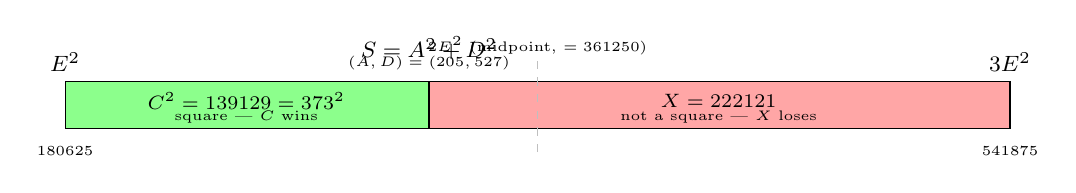
\begin{tikzpicture}[font=\footnotesize]
  \fill[green!45!white] (0,0) rectangle (4.62,0.6);
  \fill[red!35!white] (4.62,0) rectangle (12,0.6);
  \draw (0,0) rectangle (12,0.6);
  \draw[thick] (4.62,0) -- (4.62,0.6);
  \draw[gray!50, dashed] (6,-0.3) -- (6,0.9);
  \node[font=\tiny] at (6,1.05) {$2E^2$ (midpoint, $=361250$)};
  \node[above] at (0,0.6) {$E^2$};
  \node[below, font=\tiny] at (0,-0.1) {$180625$};
  \node[above] at (12,0.6) {$3E^2$};
  \node[below, font=\tiny] at (12,-0.1) {$541875$};
  \node[above] at (4.62,0.75) {$S=A^2+D^2$};
  \node[above, font=\tiny] at (4.62,0.62) {$(A,D)=(205,527)$};
  \node[font=\scriptsize] at (2.3,0.35) {$C^2=139129=373^2$};
  \node[font=\tiny] at (2.3,0.15) {square --- $C$ wins};
  \node[font=\scriptsize] at (8.3,0.35) {$X=222121$};
  \node[font=\tiny] at (8.3,0.15) {not a square --- $X$ loses};
\end{tikzpicture}
\end{center}

Drawn to scale, the asymmetry is visible directly: $S$ sits well below
the $2E^2$ midpoint for this $(A,D)$, so $X$'s segment is the larger of
the two, purely as a consequence of where $S$ happens to fall --- not
of any contest between the segments themselves.

\section{A Parity Obstruction, and the Role of $p \equiv 1 \pmod 4$}\label{sec:parity}

The search of Section~\ref{sec:partner} fixes $E$ and one opposite pair
--- say $A$, with $I$ its automatic partner --- and then probes a
second root, $C$, over a range of integers, checking whether the
resulting $X$, $F^2$, $H^2$, $D^2$, $B^2$ happen to be perfect squares.
We show that this probe may be restricted to odd $C$ without loss, and
relate the underlying mechanism to the classical condition on prime
factors of $E$ governing representations of $2E^2$.

\begin{lemma}\label{lem:oddpair}
If $E$ is odd and $u,v$ are positive integers with $u^2+v^2=2E^2$, then
$u$ and $v$ are both odd.
\end{lemma}

\begin{proof}
Since $E$ is odd, $E^2 \equiv 1 \pmod4$ and $2E^2 \equiv 2 \pmod4$.
Squares are $\equiv 0$ or $1 \pmod4$ according as their root is even or
odd. If $u,v$ have opposite parity, $u^2+v^2 \equiv 0+1 = 1 \pmod4$; if
both are even, $u^2+v^2 \equiv 0 \pmod4$. Neither matches $2 \pmod4$, so
$u,v$ must both be odd.
\end{proof}

Consequently, for odd $E$, every entry $A$ that occurs as one member of
a genuine integer pair $(A,I)$, $(D,F)$, or $(H,B)$ is itself odd; this
is why every value appearing in the representation lists of
Section~\ref{sec:cone} (for instance $205,565,289,527$ at $E=425$, and
all thirteen pairs at $E=1105$) is odd.

\begin{proposition}\label{prop:parity}
Fix odd $E$ and odd $A$ with $A^2+I^2=2E^2$ for some integer $I$, and
let $C$ be any positive integer with $C \ne A, E$, giving
$X = 2E^2-C^2$ and the forced cells of
\eqref{eq:C}--\eqref{eq:F}. If $C$ is even, then $X$, $F^2$, and $B^2$
are each $\equiv 2 \pmod4$, hence none of $X$, $F$, $B$ can be a perfect
square.
\end{proposition}

\begin{proof}
With $E,A$ odd, $E^2\equiv A^2\equiv1\pmod4$, so $2E^2\equiv2\pmod4$.
If $C$ is even, $C^2\equiv0\pmod4$, so
$X = 2E^2-C^2 \equiv 2 \pmod4$. Then
\[
F^2 = A^2+X-E^2 \equiv 1+2-1 = 2 \pmod4, \qquad
B^2 = E^2-A^2+X \equiv 1-1+2 = 2 \pmod4 .
\]
Since no perfect square is $\equiv2\pmod4$, neither $F^2$ nor $B^2$ can
be square, and $X$ itself, being $\equiv2\pmod4$, cannot be square
either.
\end{proof}

\begin{corollary}\label{cor:parity5}
Under the hypotheses of Proposition~\ref{prop:parity}, if $C$ is even
then at most six of the nine cells can be perfect squares: the four
guaranteed cells $E,A,I,C$, together with at most $H$ and $D$, since
$H^2 = E^2+A^2-X \equiv0\pmod4$ and
$D^2 = 3E^2-A^2-X\equiv0\pmod4$ remain admissible residues. In
practice the ceiling is lower still: an exhaustive search at $E=425$
and $E=1105$ found no even $C$ exceeding five squares in total.
\end{corollary}

Odd $C$ carries no such obstruction --- all four of $X,F^2,H^2,D^2,B^2$
are admissible residues in that case --- and it is exactly among the
odd probes that the seven-square example of Section~\ref{sec:ex} is
found: there, $A=205$ and $C=373$ are both odd, and three of the four
remaining cells ($H^2=529$, $D^2=277729$, $F^2=83521$) land on perfect
squares simultaneously, while only $X=222121$ fails.

\begin{remark}
Proposition~\ref{prop:parity} halves the search: for odd $E$, only odd
values of the probe $C$ need be tested, since even $C$ is provably
incapable of reaching the closing cells $X$ or $B$, and is empirically
no better than the guaranteed baseline for $H,D$ either. This is a
genuine pruning rule, established unconditionally by parity, in the
same spirit as Proposition~\ref{prop:threshold}'s positivity bound.
\end{remark}

We now turn to a coarser but prior question: whether a genuine
(non-degenerate) integer pair $A,I$ exists at all. By the classical
theorem on sums of two squares, $2E^2$ admits a representation as a sum
of two \emph{distinct} positive squares if and only if $E$ has at least
one prime factor $p\equiv1\pmod4$; the number of essentially distinct
representations grows with the number and multiplicity of such primes,
as recorded in Section~\ref{sec:rotation}. Three worked centres
illustrate how loosely this richness controls the attainable square
count.

\begin{center}
\begin{tabular}{lccc}
\hline
$E$ & factorisation & representations of $2E^2$ & best square count found \\
\hline
$425$  & $5^2 \cdot 17$      & $7$  & $7$ \\
$1105$ & $5 \cdot 13 \cdot 17$ & $13$ & $6$ \\
$422$  & $2 \cdot 211$       & $0$  & $5$ \\
\hline
\end{tabular}
\end{center}

At $E=422$, $211$ is prime and $211\equiv3\pmod4$; since $211$ divides
$E$ to an odd power and no prime $\equiv1\pmod4$ divides $E$ at all,
$2E^2$ admits no non-trivial representation as a sum of two squares.
No pair $(A,I)$, $(D,F)$, or $(H,B)$ can therefore ever consist of two
distinct positive integers, and the search collapses to isolated single
squares chosen independently, capping the total well below what $425$
or $1105$ achieve despite $422$ being a comparably sized centre.

Conversely, $1105$ has \emph{more} representations than $425$ ---
three distinct primes $\equiv1\pmod4$ against $425$'s two --- yet an
exhaustive search over every representation-pair and every odd probe
$C$ (Corollary~\ref{cor:parity5}) found no configuration exceeding six
squares, short of $425$'s seven. Richness of representation is
therefore necessary in the weak sense of Proposition~\ref{prop:parity}
and its corollary --- without it, as $422$ shows, the ceiling drops
sharply --- but it is not sufficient: whether a \emph{specific} pairing
of two representations (or of one representation with an unrestricted
odd probe) also satisfies the forced linear relations of
\eqref{eq:C}--\eqref{eq:F} is a finer question that the count of
representations alone does not answer.

\section{The Maximum Spread, and an Obstruction When $\sigma_{\text{real}}=\delta_{\text{real}}$}\label{sec:maxspread}

The walk-from-$E^2$ decomposition of Section~\ref{sec:norm} orders the
nine cells as
\[
H^2=E^2-3\delta_{\text{real}}-\sigma_{\text{real}}, \ \ldots, \ E^2,
\ \ldots, \ B^2=E^2+3\delta_{\text{real}}+\sigma_{\text{real}} ,
\]
with $H^2$ the smallest cell and $B^2$ the largest. Positivity of the
whole configuration is therefore governed entirely by $H^2$.

\begin{proposition}[The maximum spread]\label{prop:maxspread}
All nine entries are positive if and only if
\[
3\delta_{\text{real}} + \sigma_{\text{real}} < E^2 ,
\]
equivalently, in terms of the scale $S$ and ratio $t$ of
Sections~\ref{sec:independentscales} and~\ref{sec:param},
\[
S < \frac{2E^2}{2-t} .
\]
\end{proposition}

\begin{proof}
Since $\delta_{\text{real}},\sigma_{\text{real}}>0$ in the normalised
ordering, $H^2=E^2-3\delta_{\text{real}}-\sigma_{\text{real}}$ is the
smallest of the nine cells and every other cell exceeds it; hence
$H^2>0$ is necessary and sufficient. Substituting
$\delta_{\text{real}}=\tfrac{1-t}{2}S$ and
$\sigma_{\text{real}}=\tfrac{2t-1}{2}S$ gives
$3\delta_{\text{real}}+\sigma_{\text{real}} =
\tfrac{S}{2}\bigl(3(1-t)+(2t-1)\bigr) = \tfrac{S}{2}(2-t)$, and
$\tfrac{S}{2}(2-t) < E^2$ rearranges to $S < 2E^2/(2-t)$.
\end{proof}

At $E=425$: $3\delta_{\text{real}}+\sigma_{\text{real}} =
3(41496)+55608 = 180096 < 180625 = E^2$, close to the ceiling ---
consistent with $H^2=529$ being by far the smallest of the nine cells.

The two real gaps $\delta_{\text{real}}$ and $\sigma_{\text{real}}$
need not be equal, and the difference between them is not incidental.

\begin{proposition}[An obstruction at $\sigma_{\text{real}}=\delta_{\text{real}}$]\label{prop:sigmaequaldelta}
If $\sigma_{\text{real}}=\delta_{\text{real}}\neq0$, no configuration
with all nine entries square exists.
\end{proposition}

\begin{proof}
Write $\delta=\delta_{\text{real}}$. Under the hypothesis, the nine
cells become $E^2+k\delta$ for $k=-4,-3,\ldots,3,4$ --- an exact
arithmetic progression. If all nine were perfect squares, the four
consecutive terms at $k=-4,-3,-2,-1$, namely $H^2,A^2,F^2,C^2$, would
be four distinct perfect squares in arithmetic progression. No such
four squares exist, by Fermat's classical theorem on arithmetic
progressions of squares. Hence not all nine cells can be square.
\end{proof}

\begin{remark}[Where the forbidden line sits]
Solving $\sigma_{\text{norm}}=\delta_{\text{norm}}$, i.e.\
$t-\tfrac12=\tfrac{1-t}{2}$, gives the single value $t=2/3$, at which
\[
\delta_{\text{real}} = \sigma_{\text{real}} = \frac{S}{6} ,
\]
for whatever scale $S$ the configuration has: $S$ cancels from the
equality condition, so it is $t=2/3$ alone, independent of $S$, that
marks the forbidden line of Proposition~\ref{prop:sigmaequaldelta}.
\end{remark}

\begin{remark}
The square of Section~\ref{sec:ex} shows why the hypothesis matters.
There, $H^2$, $F^2$, $E^2$, $D^2$ are all four square
($23^2,289^2,425^2,527^2$), which is possible only because they do
\emph{not} lie in arithmetic progression --- their consecutive gaps are
$82992$, $97104$, $97104$, not a constant. Forcing
$\sigma_{\text{real}}=\delta_{\text{real}}$ would make all three gaps
equal to $82992$, placing $H^2,F^2,E^2,D^2$ in exact arithmetic
progression and, by Proposition~\ref{prop:sigmaequaldelta}'s argument,
making it impossible for $H^2,F^2,D^2$ to remain square alongside
$E^2$. The two independent scales are therefore not a redundancy in
the parametrisation: their inequality is precisely what keeps the
configuration clear of Fermat's obstruction, narrowing the search for
nine squares to the region $\sigma_{\text{real}}\neq\delta_{\text{real}}$
--- a genuine, if partial, answer to where the configuration of
Section~\ref{sec:cone} cannot be found.
\end{remark}

\begin{remark}[The obstruction is arithmetic, not structural]
Setting $\sigma_{\text{real}}=\delta_{\text{real}}$ does not violate
any magic-square condition: every row, column, diagonal, and
opposite-pair identity holds identically for all values of
$\delta_{\text{real}}$ and $\sigma_{\text{real}}$, by the linear
parametrisation of Section~\ref{sec:param}. The line
$\sigma_{\text{real}}=\delta_{\text{real}}$ produces a perfectly valid
magic square of integers; Proposition~\ref{prop:sigmaequaldelta} rules
it out only on squareness, via Fermat's theorem, not on any structural
ground.
\end{remark}

\begin{corollary}[Distance from the forbidden line]\label{cor:fermatdistance}
\[
\sigma_{\text{real}} - \delta_{\text{real}}
= \left(\sigma_{\text{norm}}-\delta_{\text{norm}}\right) S
= \frac{3t-2}{2}\,S .
\]
\end{corollary}

\begin{proof}
$\sigma_{\text{norm}}-\delta_{\text{norm}}
= \left(t-\tfrac12\right) - \tfrac{1-t}{2} = \tfrac{3t-2}{2}$; multiply
by $S$.
\end{proof}

At $E=425$: $\tfrac{3t-2}{2} = \tfrac{14}{275}$, and
$\tfrac{14}{275}\cdot277200 = 14112 = 55608-41496$, matching
$\sigma_{\text{real}}-\delta_{\text{real}}$ exactly. This single
normalised quantity, $\tfrac{3t-2}{2}$, measures how far a given
configuration sits from the line
$\sigma_{\text{real}}=\delta_{\text{real}}$ that
Proposition~\ref{prop:sigmaequaldelta} forbids: zero on the forbidden
line itself, and $14112$, in real units, for the square of
Section~\ref{sec:ex}.

\section{Conclusion}

The family of $3\times3$ magic squares is a three-parameter linear
family. We have given its complete parametrisation
\eqref{eq:C}--\eqref{eq:F}, shown that the associated system has rank
$6$ and nullity $3$, and exhibited a basis for its solution space.
Every relation among the cells derivable from the magic conditions is a
combination of these six, and holds identically on the family. It
follows (Theorem~\ref{thm:nolinear}) that no linear relation can be
violated by requiring the entries to be perfect squares --- which
accounts for a persistent feature of algebraic approaches to the
problem, namely that successive elimination yields correct relations
closing at $11E^2$, $9E^2$, $7E^2$, $5E^2$, $3E^2$ and $E^2$, none of
which excludes any configuration.

Recast in the anchors $(E^2, I^2, X)$, three of the cells take the
symmetric form \eqref{eq:Ba}--\eqref{eq:Fa}, and the configuration is
the medial triangle of $B^2$, $D^2$, $F^2$. Up to similarity the whole
family is one-dimensional, parametrised by a single ratio $t$. The
cells $B^2$ and $X$ close the configuration: once the other seven are
fixed, these two are determined, and whether they are squares is not
settled by the linear structure.

The arithmetic content is isolated in
Section~\ref{sec:cone}: a nine-square magic square exists if and only
if some integer $e$ admits four essentially distinct representations of
$2e^2$ as a sum of two squares, subject to the single linear condition
$a^2 + b^2 + c^2 = 3e^2$. Equivalently, four lattice points on the
circle $u^2 + v^2 = 2e^2$, related by the Gaussian rotations of
Section~11 and constrained by one plane. Since the number of such
representations is governed by the primes $p \equiv 1 \pmod 4$ dividing
$e$, this is a question about representations by sums of two squares,
not about the geometry of the square.

Two further results are unconditional.
Proposition~\ref{prop:threshold} gives the admissibility bound
$A^2 > \lvert X - E^2\rvert$, which holds regardless of squareness and
may be used to prune a search in advance. And the reflection exchanging
$A^2$ with $I^2$ preserves the multiset of entries, so the number of
square cells is invariant under it, permitting the normalisation
$A < E$.

The maximum number of perfect squares known to occur in a $3 \times 3$
magic square remains seven, realised by the square of Bremner and
Sallows, whose two non-square entries occupy the closing cells $B^2$
and $X$.

The walk-from-$E^2$ decomposition of Section~\ref{sec:norm} makes the
asymmetry between these two closing cells precise. Writing every cell
in terms of $E^2$ and the two real gaps $\delta_{\text{real}}$,
$\sigma_{\text{real}}$, only $C^2=E^2-\delta_{\text{real}}$ and
$X=E^2+\delta_{\text{real}}$ depend on $\delta_{\text{real}}$ alone;
every other cell, $B^2$ included, depends on both
$\delta_{\text{real}}$ and $\sigma_{\text{real}}$. Once the seed
$(A,D)$ --- equivalently $\delta_{\text{real}}$ and
$\sigma_{\text{real}}$ --- is fixed, $X$'s value, and so its
squareness, is already settled, with no remaining freedom to correct
it; $B^2$, by contrast, still depends on $\sigma_{\text{real}}$ and
simply fails to be square for this particular seed. This is the same
asymmetry stated in Section~\ref{sec:closedform}: squareness of $C^2$
and squareness of $X$ are two independent conditions on the same
$\delta_{\text{real}}$, so demanding both amounts to requiring $X$
itself to already lie among the finitely many members of $\mathcal
P(E)$ --- not a fault of the search, but a rigidity built into which
cells $\sigma_{\text{real}}$ can and cannot reach.

Whether eight or nine are attainable is open. What the present
analysis establishes is where the question does \emph{not} reside: not
in the linear relations among the cells, which are fully understood and
uniformly satisfied, but in the arithmetic of a single integer $2e^2$
and the lattice points of the circle it defines.

\section*{Acknowledgments}

Computational verification, review, and drafting of this manuscript
were carried out with the assistance of Claude (Anthropic).

\end{document}